%----- Preamble ----------------------------------
\documentclass[a4paper,12pt]{book}
\usepackage[T1]{fontenc}
\usepackage[latin1]{inputenc}
\usepackage{color}
\usepackage{verbatim}
\usepackage{fancybox}
\usepackage[alsoload=binary, mode=text,loctolang={DE:german},decimalsymbol=comma]{siunitx}	% Units (bit, byte and so on)
\usepackage{../Common/Tools}
\usepackage{../Common/Styles}
\usepackage[dvipdfm]{graphicx}
\usepackage{textcomp}
\flushbottom

\sloppy	% Avoid writing over linebreak
\hbadness=10000
\clubpenalty = 10000 % schliesst Schusterjungen aus
\widowpenalty = 10000 % schliesst Hurenkinder aus

% Links
\usepackage[dvipdfm, colorlinks=true, urlcolor=black, linkcolor=black]{hyperref}
\urlstyle{same} % Use normal font for Urls
\usepackage[all]{hypcap} % Link to the image, not the image caption

% Table
\usepackage{tabularx}
\usepackage{threeparttablex}
\usepackage{booktabs}
\usepackage{ltxtable}

% Code listening
\usepackage{color,listings}
\definecolor{darkgreen}{rgb}{0,0.5,0}
\definecolor{lightgray}{gray}{0.95}
\lstset{language=C++,
captionpos=b,
frame=single,
basicstyle=\ttfamily,
keywordstyle=\color{blue},
commentstyle=\color{darkgreen},
stringstyle=\color{red},
backgroundcolor=\color{lightgray},
numbers=left,
numberstyle=\tiny,
numbersep=5pt,
breaklines=true,
showstringspaces=false,
columns=fullflexible,	% Please, don't change e.g. "export ANDROID_SDK=~/android-sdk-linux_x86" into "export ANDROID_SDK =~/ android -sdk - linux_x86"
tabsize=2,
emph={double,bool,int,unsigned,char,true,false,void},
emphstyle=\color{blue},
emph={Assert,Test},
emphstyle=\color{red},
emph={[2]\using,\#define,\#ifdef,\#endif}, emphstyle={[2]\color{blue}}
}
	% "input" instead of "include" is used to avoid problems with write permissions during TeX processing
\begin{document}


%----- Title -------------------------------------
%----- Title -------------------------------------
\thispagestyle{empty}
\begin{center}

{\Huge \textbf{PixelLight PLScene documentation}}\\
%----- Title -------------------------------------
\thispagestyle{empty}
\begin{center}

{\Huge \textbf{PixelLight PLScene documentation}}\\
%----- Title -------------------------------------
\thispagestyle{empty}
\begin{center}

{\Huge \textbf{PixelLight PLScene documentation}}\\
\input{../Common/Title}

\end{center}


\end{center}


\end{center}

\tableofcontents
\cleardoublepage


%----- Document ----------------------------------
\chapter{Introduction}


\paragraph{Motivation}
The PixelLight math component provides common required tools like vector and matrix classes and therefore implements features, which are especially useful when dealing this 3D graphics.




\section{External Dependences}
PLMath only depends on the \textbf{PLCore} library and doesn't use any external third party libraries.




\section{Transforming 2D to 3D and reversed}


\paragraph{Overview}
Sometimes it's required to project a 3D world position onto the screen to get the 2D x/y display position of it or you want to find out on which 3D world position a 2D position is on. This can be seen as the interface between the flat 2D screen and the 3D world.


\paragraph{3D to 2D}
\emph{Vector3::To2DCoordinate()} returns the 2D screen coordinate corresponding to a given 3D world coordinate using the given camera settings. This can be useful if you e.g. want to set the mouse cursor over a given 3D object.


\paragraph{2D to 3D}
\emph{Vector3::To3DCoordinate()} returns the 3D coordinate corresponding to a given 2D screen coordinate using the given camera settings. 2D to 3D transformation is extremely useful if you want to perform picking were the user is able to select a 3D object by using the mouse. Because picking is a collision task were we have to find the intersection point of the line (camera position to mouse position) and the meshes, this is not handled in this document. Have a look at the \emph{PixelLight API documentation} for more information how to perform picking.





\section{Additional tool functions}
\emph{PlaneSet::CreateSelectionPlanes()} takes a 2D start and end point and will return a plane set with the \emph{selection planes}. This plane set can be seen as \emph{selection frustum} and you can test your objects against it to see what's selected and what's not.

\cleardoublepage
\chapter{General}




\section{Keep it Simple!}
The world is complicated enough - if there are multiple solutions, prefer the simplest over the most complicated one! This way, the chances are high that other will understand the solution as well as you when looking at the code some years later.




\section{Encoding}
We work with multiple operation systems so we have to take into account \emph{how} text files are saved. All \emph{Diary}, \emph{Readme}, \emph{Todo} and \emph{Plan} text files saved as "Unicode (UTF-8 with signature) - Codepage 65001". All other text files like code or make files saved in classic \emph{ANSI}.




\section{File Extension}
First of all, we use the old fashion \emph{.h}-file extension to mark header files - \emph{hpp} would be the \emph{correct} extension for C++, but it's not widely used. Usually, we outsource inline implementations into files with an \emph{inl}-extension to keep the header files good readable. For source codes, we use the file extension \emph{cpp}.




\section{C++11 Language Features}
Using C++11 (previously known as C++0x) language features is fine as long as
\begin{itemize}
\item{It's possible to emulate, or at least deactivate the feature within compilers don't supporting it (yet)}
\item{There's no comfortable/acceptable way to solve a task without using the feature, but those situations have to be discussed within the team and community}
\end{itemize}
\textsl{}
Currently the following C++11 language features are used:
\begin{itemize}
\item{\emph{nullptr} - a null pointer literal}
\item{\emph{override} - gives the compiler a chance to detect and blame errors related to overwriting methods}
\end{itemize}


\paragraph{Extern Templates}
Don't use \emph{extern templates}\footnote{\url{http://www2.research.att.com/~bs/C++0xFAQ.html\#extern-templates}} in order to avoid template instantiation in other modules. This is a feature we can't emulate and there are still legacy compilers like \ac{GCC} 4.2.1 used on Mac OS X 10.6 actively used around the world. So, at least for now, don't use this useful feature.




\section{For-Scope}
Within the PixelLight projects, the \emph{for-scope} is active by default. The following for instance will produce a compiler error:
\begin{lstlisting}[caption=for-scope]
for (int i=0; i<1; i++) {
	// Do anything
}
i = 20;	// i has already gone out of scope
\end{lstlisting}




\section{Null Pointer}
For null pointers, use \emph{nullptr}\footnote{For example \emph{Microsoft Visual Studio 2010} and \emph{\ac{GCC} 4.6} have native support for \emph{nullptr}} from \emph{C++11} and not for example the legacy, but traditional \emph{NULL} definition or even directly a integer $0$.

\begin{lstlisting}[caption=Null pointer]
char *pszMyString = nullptr;
\end{lstlisting}




\section{Overwriting Methods}
Put the methods within the base class, which are allowed to be overwritten, into a separate code block so everyone is able to find them at once.
\begin{lstlisting}[caption=Virtual methods within a base class]
//[-------------------------------------------------------]
//[ Public virtual MyClass functions                      ]
//[-------------------------------------------------------]
virtual void MyMethod() = 0;
\end{lstlisting}

When overwriting virtual methods within a derived class, put the overwritten methods into a code block telling were those methods originally came from.
\begin{lstlisting}[caption=Overwriting virtual methods within a derived class]
//[-------------------------------------------------------]
//[ Public virtual MyClass functions                      ]
//[-------------------------------------------------------]
virtual void MyMethod() override;
\end{lstlisting}
Although technically not required, do also add a \emph{virtual} to make it absolutely clear that this is a virtual method. To give the compiler a chance to find and blame possible errors like a signature change within the base class, use the C++11 language keyword \emph{override}.




\section{Casting}
PixelLight is using \emph{C++ style casts} (\emph{int i = static\_cast<int>(42.21f)}), not \emph{C style casts} (\emph{int i = (int)42.21f}). It's much easier to search for \emph{C++ style casts}\footnote{\emph{static\_cast}, \emph{reinterpret\_cast}, \emph{const\_cast}, and \emph{dynamic\_cast}} and they are less vulnerable to unintended effects as well - and because they are not that compact as the \emph{C style casts}, one may think about it a second time why there's a need for a cast.

\paragraph{\ac{GCC}}
\ac{GCC}, offers an option called \emph{-Wold-style-cast} to let the compiler warn if an old-style (C-style) cast to a non-void type is used within a C++ program.




\section{Const Correctness}
Define functions, variables etc. whenever possible to be constant. By giving the compiler this hint, it may be possible to use special optimizations or uncover bugs within the implementation.


\paragraph{Const Example}
Have a look at the following example function:
\begin{lstlisting}[caption=Non-constant function parameter]
void MyFunction(PLMath::Vector3 &vPosition)
{
	// ...
}
\end{lstlisting}
In case the function is considered to manipulate \emph{vPosition}, all's fine. Let's continue with another usage example:
\begin{lstlisting}[caption=Using a temporary variable instance as non-constant function parameter]
MyFunction(PLMath::Vector3(0.0f, 1.0f, 2.0f));
\end{lstlisting}
The compiler creates a temporary \emph{PLMath::Vector3} instance on the runtime stack and is passing a reference into the function. Looks fine as well? In case the function manipulates the variable passed by reference, the temporary instance is changed. In principle that's no problem because it's thrown away after the function call anyway. In practice, this situation is considered to be evil. \ac{MSVC} 2010 will shy tell you via a warning
\begin{quote}warning C4239: nonstandard extension used : 'argument' : conversion from 'PLMath::Vector3' to 'PLMath::Vector3 \&' A non-const reference may only be bound to an lvalue\end{quote}
So, it's possible to just ignore or even deactivate this warning... isn't it? In fact, it isn't because other compilers might not be that tollerant and will throw an error message at you. To sum this up: In the example above, you really want to write
\begin{lstlisting}[caption=Constant function parameter]
void MyFunction(const PLMath::Vector3 &vPosition)
{
	// ...
}
\end{lstlisting}
in order to be cross-platform safe.


\paragraph{Const Exception}
There's one situation were we do not use \emph{const} - when dealing with function parameters because

\begin{lstlisting}[caption=Function parameters]
void MyFunction(int nVariable1, int nVariable2);
\end{lstlisting}

is inside headers better readable than

\begin{lstlisting}[caption=Constant function parameters]
void MyFunction(const int nVariable1, const int nVariable2);
\end{lstlisting}

In this situation, the readability is more important for us. This rule does not apply for pointer or reference parameters like

\begin{lstlisting}[caption=Constant function pointer/reference parameter]
void MyFunction(const String &sVariable);
\end{lstlisting}

because the user should be able to see whether or not a function is going to manipulate the parameter variable!




\section{static const Vs. const static}
Use \emph{static const} instead of \emph{const static}. Have a look at e.g. the \ac{GCC} option \emph{Wold-style-declaration} resulting in the warning \begin{quote}`static' is not at beginning of declaration\end{quote} or into chapter 6.11 of ISO C99 (\emph{Future Language Directions} -> \emph{Storage-class specifiers}).




\section{Namespaces}
PixelLight is using multiple namespaces, one for each sub-project. If you want to use for instance the string class which is defined in \emph{PLCore} you need to do this:

\begin{lstlisting}[caption=Explicit namespace]
PLCore::String sMyString;
\end{lstlisting}

Or this:

\begin{lstlisting}[caption=Using namespace]
using namespace PLCore;
...
String sMyString;
\end{lstlisting}

Try to avoid using \emph{using namespace} too often or this will result in name conflicts which you then have to resolve by hand by adding for instance \emph{PLCore::}. We recommend to never use \emph{using namespace} within header files!




\section{Dynamic Parameters}
When dynamic parameters are used and the name of the parameters inside a string is irrelevant, as this is the case for \emph{PLCore::Params::FromString}, the parameters are named using \emph{Param<x>} were x starts with $0$ (example: \emph{Param0=1 Param1=''Hello''}).  




\section{Names}
In general, names of classes, functions, variables and so on must have human readable names. The name has to tell as much as possible about the usage - if the user can guess correctly the usage of for example a variable by just looking at it's name, the name is perfect.

General rules:

\begin{itemize}
\item A single character as name for local (only local!) control variables like \emph{i} within a for-loop is acceptable as long as there are not to much of those at once (else use reasonable names to avoid confusion!)
\item Short cuts should be avoided whenever possible because they may leads to confusion\footnote{True story: When using \emph{Rot} as short cut for \emph{Rotation}, we once had the situation that a German speaking programmer asked confused what the color \emph{Rot} should do inside the scene node... in German, \emph{Rot} is the word for \emph{red}...} (NO stuff like \emph{stricmp()}!)
\item If there's a \emph{commonly used} name for something, just this name instead of creating a totally new one
\item Avoid long names, if there's an expressive shorter name it's the preferred one... but keep the short cut rule in mind!
\end{itemize}

Classes, structures and so on have a upper case letter at the beginning. Example:

\begin{lstlisting}[caption=Name convention]
class Player {
};
struct Info {
};
\end{lstlisting}




\section{Prefix}
Because the readability of code is extremely important when working in a team and/or using code from others, one of our goals was to make the PixelLight code as readable and well structured as possible. We are using a name style convention\footnote{We know that there are a lot of discussions around the internet whether or not prefixes should be used. In the year 2002 we decided to use them and we don't change it - due to the dimension of the PixelLight project, it would be a huge effort to change it anyway.}.

Variable prefixes for standard types:

\begin{lstlisting}[caption=Variable prefixes for standard types]
Type               Prefix    Example
bool               b         bool bActive

(n for all none standard floating point types)
int                n         int  nNumber
char               n         char nCharacter
long               n         long nHuge

float              f
double             d

(Character arrays -> strings)
char[]             sz        char szName[64]
char*              psz       char *pszName

(Pointers)
*                  p         Player *pPlayer

(References)
&                  -         char &nTest = nTest2;

struct instance    s         Info sPlayer (struct Info)

class instance     c         Player cPlayer (class Player)
\end{lstlisting}

General variable prefix for class variables:
m\_ (m for member)\\
Example: char *m\_pszName\\

Variable prefixes for PixelLight types:

\begin{lstlisting}[caption=Variable prefixes for PixelLight types]
Type               Prefix    Example
String             s         String sName

Container          lst       List lstNames

Map                map       HashMap mapNames

VectorX            v         Vector3 vPosition
(X for dimension: 2, 3 or 4)

MatrixXxX          m         Matrix4x4 mRotation
(X for dimension: 3 or 4)

Quaternion         q         Quaternion qRotation

ColorX             c         Color3 cColor (same as class)
(X for dimension: 3 or 4)
\end{lstlisting}




\section{Postfix}
We recommend you to use the PixelLight name convention and marking debug versions with a \emph{D} at the end of the filename. Example: \emph{MyPlugins.dll} = release version, \emph{MyPluginsD.dll} = debug version.




\section{Events and Signals}
As soon as an event is inside a class, we refer to it as \emph{signal}. As such, the prefix \emph{Event} like within \emph{EventKeyDown} is used outside classes while prefix \emph{Signal} like within \emph{SignalKeyDown} is used inside classes.




\section{Event Handlers and Slots}
Within our name convention for event handlers and \ac{RTTI} slot names, there's a \emph{On} within for example \emph{OnMyEvent} indicating that this is a handler/slot method. The other part of the name consists of the name of the event/signal - for \emph{OnMyEvent} this would be an event/signal with the name \emph{MyEvent}.




\section{\ac{RTTI} Interface}
Within PixelLight, the \ac{RTTI} class properties and members are always defined in the following order:
\begin{itemize}
\item Properties
\item Attributes
\item Constructors
\item Methods
\item Signals
\item Slots
\end{itemize}
This way one knows exactly were to look for something. Further, within the \ac{RTTI} class properties and members definitions, only tabs and no spaces are used to make it easier to write the definitions like a table. This makes it more comfortable for the eyes and brain to navigate to certain definition parts without to much searching around.

Here's an example source code showing the common \ac{RTTI} interface layout (without the word wrap):
\begin{lstlisting}[caption=\ac{RTTI} interface (without the word wrap)]
//[-------------------------------------------------------]
//[ RTTI interface                                        ]
//[-------------------------------------------------------]
pl_class(pl_rtti_export, MyRTTIClass, "", PLCore::Object, "Sample RTTI class, don't take it to serious")
	// Properties
	pl_properties
		pl_property("MyProperty",	"This is a property value")
	pl_properties_end
	// Attributes
	pl_attribute(Name,	PLCore::String,	"Bob",	ReadWrite,	GetSet,			"A name, emits MySignal after the name was changed",			"")
	pl_attribute(Level,	int,			1,		ReadWrite,	DirectValue,	"Level, automatically increased on get/set name and OnMyEvent",	"")
	// Constructors
	pl_constructor_0(DefaultConstructor,	"Default constructor",	"")
	// Methods
	pl_method_0(Return42,			int,					"Returns 42",							"")
	pl_method_1(IgnoreTheParameter,	void,			float,	"Ignores the provided parameter",		"")
	pl_method_0(SaySomethingWise,	void,					"Says something wise",					"")
	pl_method_0(GetSelf,			MyRTTIClass*,			"Returns a pointer to this instance",	"")
	// Signals
	pl_signal_1(MySignal,	PLCore::String,	"My signal, automatically emitted after the name was changed",	"")
	// Slots
	pl_slot_0(OnMyEvent,	"My slot",	"")
pl_class_end
\end{lstlisting}



\section{Reuseability and adding new Stuff}
Before you add new classes, functions an so on - check first whether there's already something similar within PixelLight. If there's something you can already use directly, use it instead of writing new stuff. If there's something quite similar, have a more detailed look at it and contact your team colleagues to discuss whether a refactoring is possible and reasonable to update and/or to enhance existing stuff.

Reuseability is one of the most important concepts when creating frameworks like PixelLight... and reuseability does not mean that it's possible to copy'n'past it and then hacking around for a certain project! Reuseability means that it's possible to directly reuse, to share, something between multiple projects in a quite universal way without the need to enhance and hack around constantly!

\cleardoublepage
\chapter{PLCore}


\paragraph{Motivation}
\emph{PLCore} is the most basic library of PixelLight. In here, you'll find container implementations like linked lists, arrays up to hash maps. Strings, files, checksum, XML, log and interfaces for the general interaction with the used operation system are also available. Usually, every PixelLight basing project is using \emph{PLCore} features because they are just essential and by using it, one can avoid to implement linked lists, strings etc. multiple times within multiple projects which would just be inefficient and error prone.\footnote{When using external third party libraries, it's usually fact that they implement their own linked lists, strings and so on - this shouldn't be the case for PixelLight based projects.}

The PixelLight core component also provides more advanced features that are usually quite useful for all types of projects. As the project name \emph{PLCore} implies, it's the foundation of the PixelLight framework which is used for the development of complete applications. RTTI, plugins, the application framework.


\paragraph{Overview}
The heart of PLCore is the RTTI which is completely basing on C++ templates and additionally offers some macros to enhance the readability and usability. By using C++ templates, the system is type safe. The RTTI is using several fundamental components like variables, functions, events and event handler. This components, the RTTI is composed of, can be subdivided into three levels as summarized within table~\ref{Table:FundamentalRTTIComponents}.
\begin{table}[htb]
	\centering
	\begin{tabular}{|l||l|l|l|}
		\hline
		Components & 1. Virtual Base Class & 2. Typed Variant & 3. Inside Object\\
		\hline
		\hline
		Variable & DynVar & Var\textless type\textgreater & Attribute\textless type\textgreater\\
		\hline
		Function & DynFunc & Func\textless type\textgreater & Method\textless type\textgreater\\
		\hline
		Event & DynEvent & Event\textless type\textgreater & Signal\textless type\textgreater\\
		\hline
		EventHandler & DynEventHandler & EventHandler\textless type\textgreater & Slot\textless type\textgreater\\
		\hline
	\end{tabular} 
	\caption{Fundamental RTTI components and their levels}
	\label{Table:FundamentalRTTIComponents}
\end{table}




\section{External Dependences}
\emph{PLCore} is using some open source third party libraries which are static linked. As a result, the resulting \emph{PLCore} library has no additional external shared library dependencies.


\paragraph{zlib}
\begin{itemize}
\item ZIP library
\item \emph{zlib} license
\item Version \emph{1.2.3}
\item Used by the zip file classes
\item Downloaded from \url{http://www.zlib.org/}
\end{itemize}


\paragraph{PCRE}
\begin{itemize}
\item Regular expression library
\item \emph{BSD} license
\item Version \emph{8.10}
\item Used by the \emph{RegEx} class
\item Downloaded from \emph{http://www.pcre.org/}
\end{itemize}




% Include the other sections of the chapter
\section{String}




\subsection{String Class}
Sequences of characters, also called \emph{strings}, are often used and frequently come with some nasty features like memory leaks, buffer overruns (security risk!) or even crash's if you are not careful. Also dealing with Unicode is normally not that much fun\ldots so we wrote a comfortable string class making our and especially your life much easier!

Because strings are quite fundamental, there are several optimizations in place to make dealing with strings as fast as possible. The \emph{String}-class uses a \emph{copy on change}-technique - therefore copying one string into another one is quite fast because the internal string buffer is shared as long as a string doesn't change. As result comparing strings can also be very fast and the internal string buffer can be ASCII or Unicode in a quite flexible way. To enhance the string performance, the internal string buffers are managed by a string buffer manager to avoid to many memory allocations/deallocations. For an additional performance improvement, memory is traded for speed, meaning that additional characters are allocated within the internal string buffer manager for future use. This way, appending new characters to a string is usually quite fast.

As long as you don't save your source codes in an UTF8 format you can also use the ASCII extension Ansi, meaning characters between 128-256. But with an UTF8 format, this may cause serious problems and you should use Unicode instead ASCII for characters above 128\footnote{Using codepage based ASCII is not recommended} to avoid encoding troubles!

Here's a short usage example how to use the \emph{String}-class and how do deal with ASCII/Unicode/UTF8:

\begin{lstlisting}[caption=ASCII/Unicode/UTF8 string example]
// Test string instance
PLCore::String sS;

// Set string to 'Mini' as ASCII
sS = "Mini";

// Concatenate 'Me' (ASCII) with the string
sS += " Me";

// Get pointer to ASCII string content
const char *pS = sS.GetASCII();

// Get pointer to ASCII string content
// (same as above but not recommended)
const char *pS = sS;

// Set string to 'Mini' as Unicode
sS = L"Mini";

// Set string to 'nihon' (= Japanese)
// as Unicode by using masked characters
sS = L"\u65e5\u672c\u8a9e";

// Set string to 'Mini' as UTF8
sS = PLCore::String::FromUTF8("Mini");
\end{lstlisting}

As you can see the well known \emph{char*} and \emph{wchar\_t*} are used for ASCII and Unicode strings. We strongly recommend that you don't brother yourself with this stuff as long as not necessary. So, just use \emph{String sS = "Mini";} instead of \emph{String sS = L"Mini";}. It's more readable and ASCII is more performant and requires less memory. The \emph{String}-class takes automatically care of ASCII/Unicode for you, so you can even mix strings with different internal formats!

We strongly recommend to use only this class when working with strings and not using for instance \emph{c}-functions like \emph{strcmp()}. Do also avoid to use the string data you can get from the \emph{String::GetASCII()} directly to search for substrings and so on - use the provided string functions instead. By doing so, the string class will automatically take care of tricky stuff mentioned above.

In general, it's a good idea to use functions like \emph{String::GetASCII()} to get the \emph{internal data} only if really required, for instance if the string data is given to another non PixelLight system.


\paragraph{UTF8}
Originally, the string class had native UTF8 support build in. For each \emph{char} and \emph{wchar\_t} method, there was also an equivalent UTF8 method. Because the compiler can distinguish \emph{char*} and \emph{wchar\_t} by using \emph{L} in front of strings, but not ASCII from UTF8, we introduced the \emph{utf8} data type. If the compiler should interpret a given string as UTF8, we casted it to \emph{utf8} like \emph{String sS = (const utf8*)"Mini";}.

Due to the complexity of the UTF8 implementation and the possible combinations with \emph{char} and \emph{wchar\_t} and a constant lack of time, the UTF8 implementation was not fully implemented and there were a lot of TODO-points. At the end of the year 2010 the decision was made to give up the internal native UTF8 implementation - the alternatives were to keep the unfinished string codes for some more years, or to spend some weeks in completing and testing the native UTF8 implementation... with the possibility that the resulting implementation would have a poor performance and tons of hidden bugs (waiting quietly in the dark to attack) due to it's complexity. Both options were not that attractive.

Now, the string class offers a \emph{ToUTF8}-method to return the current string content as, internally cached, UTF8 formatted string as well as a \emph{FromUTF8}-method to create a PixelLight string instance by using a given UTF8 formatted string. This two methods can be used to exchange strings with for example UNIX systems or with other \ac{API}s like Qt.


\paragraph{wchar\_t}
In contrast to UTF8, \emph{wchar\_t} is quite comfortable to use in practice because each character has the same number of bytes. But there's also a dark side... while on Microsoft Windows a \emph{wchar\_t} is two bytes long (UTF-16), it's four bytes long on UNIX systems (UTF-32). When saving a \emph{wchar\_t} string under Microsoft Windows, and loading it on a UNIX system you will get an ugly surprise (\emph{kawoom!}).

To make it even more interesting, there's a compiler flag called "wchar\_t is treated as built-in type" you may set by using \emph{Zc:wchar\_t}, or not by using \emph{-Zc:wchar\_t-}. While the one libraries, like PixelLight, are using "wchar\_t is treated as built-in type", other libraries are using the other way - resulting in incompatible libraries!

So, be carefully when using \emph{wchar\_t} to serialize data or to pass strings to other libraries, or better, don't do it and use UTF8 instead!


\paragraph{Single Characters}
If you care about best possible performance (even if nearly not measurable), use character string methods when dealing with characters - for example, write \begin{quote}String sS = 'A';\end{quote} instead of \begin{quote}String sS = "A";\end{quote}. This way, the string method already knows that you provided just a single character and don't need to count characters internally.


\paragraph{Strings and Dynamic Variable Parameters}
Often it's required to give for instance a function a string which is composed of different substrings. For instance \emph{DrawText("My text")} is trivial, \emph{DrawText("\%d: My text '\%s'", 1, "Text")} will only work if the function supports dynamic variable parameters. For PixelLight, we decided to not providing such functions with dynamic variable parameters for various reasons. Instead, one can compose own strings by hand or by using the \emph{PLCore::String}-class. With \emph{String} the previous example would look like this \emph{DrawText(String::Format("\%d: My text '\%s'", 1, "Text"))}. \emph{String::Format} will compose the string for you and there can't be a buffer overflow if the resulting string gets to long.

Here's an example how to use this string class and how not:

\begin{lstlisting}[caption=Valid and invalid string usage example]
PLCore::String sOldString = "Moin";
PLCore::String sNewString;

// Not correct! (pointer to string object
// instead of string content is used...)
sNewString = PLCore::String::Format("Old string: %s", sOldString);

// Correct
sNewString = PLCore::String::Format("Old string: %s", sOldString.GetASCII());

// Even better because for example Unicode safe
sNewString = "Old string: " + sOldString;
\end{lstlisting}

If possible, try to avoid to use this method because it's usually considered to be \emph{slow} due to it's internal complexity. Therefore, write something like
\begin{quote}String sMyString = String("The number ") + 42 + " is fantastic!";\end{quote} instead of \begin{quote}String sMyString = String::Format("The number \%d is fantastic!", 42);\end{quote}


\paragraph{Strings as Function Parameters}
When using strings as function parameters and/or return values we recommend the following solution:

\begin{lstlisting}[caption=String as function parameter and return value]
PLCore::String GetOtherString(const PLCore::String &sString);
\end{lstlisting}

The string parameter is given as reference which is quite performant as you may now. The returned string on the other hand is an object on the runtime stack - please note that this is not performance critical because the internal string data is not copied, it's only shared as long as possible! By doing so, you can avoid tricky situations like giving a function a reference to it's own internal string you received from another function of the same class.

Example:

\begin{lstlisting}[caption=Error prone string usage example]
class StringMessUp {
	public:
		const PLCore::String &GetFilename() const
		{
			return m_sFilename;
		}
		void Cleanup()
		{
			m_sFilename = "";
		}
		void Load(const PLCore::String &sFilename)
		{
			Cleanup();
			m_sFilename = sFilename;
		}
	private:
		PLCore::String m_sFilename;
};

// Somewhere in the deep of the codes...
StringMessUp cInstance;

// ...
cInstance.Load("Test.ext");
\end{lstlisting}

Often a clean up or similar is used as shown in the situation above - but in this case the programmer was careless and will get a surprise if we tests the code with \emph{cInstance.Load(cInstance.GetFilename());} for reloading. Think a moment about this\ldots right, because \emph{sFilename} is in fact a reference to the internal \emph{m\_sFilename} that is cleared within this \emph{Load()}-function before loading, \emph{sFilename} is now empty, too - and nothing is loaded.




\subsection{Regular Expression}
Regular expressions\footnote{At \url{http://www.regular-expressions.info/} are some good regular expression tutorials online available, as well as a basic syntax reference at \url{http://www.regular-expressions.info/reference.html}} are an universal and powerful tool to deal with string operations like \emph{seach for}. Here's a compact example how to use regular expressions to check whether or not a string is a substring of another one:

\begin{lstlisting}[caption=Regular expression example]
	PLCore::String sBeer = "BeerNumber99";
	PLCore::RegEx cRegEx("^BeerNumber.*$");
	if (cRegEx.Match(sBeer))
		sBeer = "Drunk";
\end{lstlisting}

Because the string \emph{BeerNumber99} matches the expression \emph{\textasciicircum BeerNumber.*\$} the beer is now gone. Strings like \emph{\_BeerNumber99} or \emph{Number99} don't match the given expression.




\subsection{Wildcard}
It's practical to only support regular expressions or wildcards, but not both - so you don't need multiple implementations. Usually it's best to support regular expressions because they are more powerful than wildcards. Wildcards on the other side are more compact and users may already be familiar with them through \emph{Microsoft Windows} - therefore we added \emph{PLCore::RegEx::WildcardToRegEx()} so one can convert a given wildcard into an regular expression\footnote{Wildcard: \emph{BeerNumber*} = regular expression: \emph{\textasciicircum BeerNumber.*\$}} and then passing this to a function.




\subsection{Qt String Adapter}
Within the project \emph{PLFrontendQt}, there's a static adapter class for mapping Qt\footnote{Qt is a cross-platform application and \ac{UI} framework, \url{http://qt.nokia.com/}} strings to PixelLight strings and vice versa.

We provide this string adapter class because it's nice to be able to use PixelLight within Qt as comfortable as possible. Please note that the existence of this adapter class doesn't mean that PixelLight depends on Qt - inside PixelLight, neither this class nor Qt are used!\footnote{That's the reason why there's just a header file for this class, and no C++ file}

The following source code example shows how to convert a Qt string to \emph{PLCore::String}.
\begin{lstlisting}[caption=Qt string to PLCore::String]
	PLFrontendQt::QString sQtString = "Qt says hello to PixelLight";
	PLCore::String sPLString = PLFrontendQt::QtStringAdapter::QtToPL(sQtString);
\end{lstlisting}

The following source code example shows how to convert \emph{PLCore::String} to a Qt string.
\begin{lstlisting}[caption=PLCore::String string to Qt]
	PLCore::String sPLString = "Greetings from PixelLight to Qt";
	PLFrontendQt::QString sQtString = PLFrontendQt::QtStringAdapter::PLToQt(sPLString);
\end{lstlisting}


\paragraph{wchar\_t}
Please note that there's a perfidy when using \emph{wchar\_t} in combination with PixelLight \& Qt...

When using the default settings within e.g. \emph{Microsoft Visual Studio 2010}, \emph{wchar\_t} is treated as built-in type, so third party unicode shared libraries usually use it. So, this is also the default setting for PixelLight projects. On the other hand, if you want to use PixelLight within Qt and write something like \begin{quote}PLCore::String sString = L"Test";\end{quote}, the linker will give you an error message like \begin{quote}error:  unresolved external symbol "\_\_declspec(dllimport) public: \_\_thiscall PLCore::String::String(unsigned short const *,bool,int)" (\_\_imp\_??0String@PLCore@@QAE@PBG\_NH@Z) referenced in function \_main\end{quote} because within Qt, \emph{wchar\_t} is defined as \emph{unsigned short} and not as build in type \emph{wchar\_t}.

One solution is to remove \emph{-Zc:wchar\_t-} from \emph{QMAKE\_CFLAGS} within \emph{qmake.conf} of Qt, and then recompiling Qt. Another solution,  is to recompile PixelLight with a set \emph{-Zc:wchar\_t-}... which means that it might be necessary to modify external dependencies as well! Both solutions are poor because they enforce to much work and potential additional conflicts! Therefore we pass over the string by using UTF8 to avoid the need to recompile PixelLight/Qt with other compiler settings.

\cleardoublepage
\section{System}




\subsection{OS console}
Within the \emph{Console}-class you can find some basis OS console functions. Those can be quite handy because even the most primitive functions can and often are different on multiple platforms! You can request an instance of this class by using the \emph{System}-class.

The following example shows how you can use some of this functions for a simple but useless application:

\begin{lstlisting}[caption=OS console usage example]
//[-------------------------------------------------------]
//[ Includes                                              ]
//[-------------------------------------------------------]
#include <PLCore/Main.h>
#include <PLCore/System/System.h>
#include <PLCore/System/Console.h>


//[-------------------------------------------------------]
//[ Namespaces                                            ]
//[-------------------------------------------------------]
using namespace PLCore;


//[-------------------------------------------------------]
//[ Program entry point                                   ]
//[-------------------------------------------------------]
int PLMain(const String &sFilename, const Array<String> &lstArguments)
{
  // Get the console
  const Console &cConsole = System::GetInstance()->GetConsole();

  // This code loops until any key is hit
  cConsole.Print("\nPress any key to quit...\n");
  while (!cConsole.IsKeyHit()) {
    // Do anything
  }

  // Read and throw away the hit key
  cConsole.GetCharacter();

  // Clear the OS console
  cConsole.ClearScreen();

  // Ask the user something
  cConsole.Print("\nDo you want a sweet goodbye? (y/n)\n");
  const int nCharacter = cConsole.GetCharacter();
  if (nCharacter == 'y' || nCharacter == 'Y') {
    cConsole.Print("Goodbye\n");

    // Wait 2 seconds
    System::GetInstance()->Sleep(2000);
  }

  // Done
  return 0;
}
\end{lstlisting}

\cleardoublepage
\section{File System}
We don't discuss each technical detail of the file system, instead we bring a number of examples and explain them. To find out the rest like creating a file by yourself should be no problem.




\subsection{File}
The rule for dealing with files is pretty simple: open, read/write, close

Let's have a look how this may look in practice:

\begin{lstlisting}[caption=File usage example]
// Create the file object and set it to the 'MyFile.my' file
File cFile("MyFile.my");

// Open the existing file to read in text
if (cFile.Open(File::FileRead | File::FileText)) {
	// Read a string from the file
	String sLine = cFile.GetS();

	// Close the file
	cFile.Close();
}

// Open the existing file to write in binary data
if (cFile.Open(File::FileWrite)) {
	// Write the byte sequence 'Blub', 1 byte per item, 4 items
	cFile.Write("Blub", 1, 4);

	// Read a string from the file
	String sLine = cFile.GetS();

	// Close the file
	cFile.Close();
}
\end{lstlisting}

After the boring example, let's open a file located in the Internet:

\begin{lstlisting}[caption=http file usage example]
// Create the file object and set it to a file inside a zip
// archive located on a http server - CRAZY... but it works
File cFile("http://www.pixellight.org/test.zip/Test/1.txt");

// Open the file to read in text
if (cFile.Open(File::FileRead | File::FileText)) {
	// Get the OS console instance
	const Console &cConsole = System::GetInstance()->GetConsole();

	// Write some start information into the OS console
	cConsole.Print("Reading content of '" +
		cFile.GetUrl().GetUrl() + "' (text):\n");

	// Read until the end of the file is reached
	while (!cFile.IsEof()) {
		// Read a line from the file
		String sLine = cFile.GetS();

		// Modify some escape codes
		sLine.Replace("\r", "\\R");
		sLine.Replace("\n", "\\N");

		// Show the read line on the OS console
		cConsole.Print("- " + sLine + '\n');
	}

	// Close the file
	cFile.Close();
}
\end{lstlisting}




\subsection{Directory and File Search}
Let's directly jump into code action, open a directory and list all files within it:

\begin{lstlisting}[caption=Directory and file search usage example]
// Open directory
Directory cDir("MyDirectory");
if (cDir.Exists() && cDir.IsDirectory()) {
	// Initialize search handle
	FileSearch cSearch(cDir);

	// Loop through all found files
	while (cSearch.HasNextFile()) {
		// Get the name of the found file
		String sName = cSearch.GetNextFile();
	}
}
\end{lstlisting}

To search for all \emph{cpp}-files just modify the file search handle a little bit:

\begin{lstlisting}[caption=Wildcard search handle]
// Initialize search handle with a wildcard
FileSearch cSearch(cDir, "*.cpp");
\end{lstlisting}

For more complex file search filters it's recommended to use a regular expressions:

\begin{lstlisting}[caption=Regular expression search handle]
// Initialize search handle with a regular expression
// (PCRE syntax)
SearchFilterRegEx cFilter("(?i)^(win|w)\\w+(32)?.(dll|exe)$");
FileSearch cSearch(cDir, &cFilter);
\end{lstlisting}




\subsection{URL}
Besides usual strings, strings which contain an URL (Uniform Resource Locator) are often even more painful to deal with because it's not as uniform as the name may indicate. \emph{Microsoft Windows} for instance is using backslashes (\textbackslash\textbackslash) to separate components while Unix systems are using slash's (/), Unix is case-sensitive while \emph{Microsoft Windows} is not, \emph{MyDirectory/Thing} can be an URL pointing to a directory named \emph{Thing} or to a file named \emph{Thing} without a file extension\ldots We think you go the idea. Because this nasty stuff frequently gave us headaches and making writing platform independent applications to a nightmare, we decided to create an \emph{Url}-class that manages this topic automatically for us so we are happy programmers again.

There are no big problems throwing around strings containing an URL, but if they are manipulated or parsed, we strongly recommend to use the \emph{Url}-class - else you have to take care of the situations mentioned above within each code dealing with URL's and this is can be very error prone and frustrating.

Here's an example of how complicated a simple \emph{get me the path, title and extension}-code can get - even with the comfortable \emph{String}-class:

\begin{lstlisting}[caption=File path\, title and extension without using the Url-class]
// A given filename
#ifdef WIN32
String sFilename = "MyDirectory\\Thing.ext";
#elif LINUX
String sFilename = "MyDirectory/Thing.ext";
#endif

// Get the path the file is in
String sPath;
int nPathIndex = sFilename.LastIndexOf('\\');
if (nPathIndex < 0)
	nPathIndex = sFilename.LastIndexOf('/');
if (nPathIndex >= 0)
	sPath = sFilename.GetSubstring(0, nPathIndex+1);

// Get the title and extension of the file
String sTitle, sExtension;
int nTitleIndex = sFilename.IndexOf('.');
if (nTitleIndex >= 0) {
	sTitle = sFilename.GetSubstring(nPathIndex+1, nTitleIndex-nPathIndex-1);
	sExtension = sFilename.GetSubstring(nTitleIndex+1);
}
\end{lstlisting}

Ugly, isn't it? And don't forget that all codes using your parsed filename parts have also to take care of the differences between operation systems! And now the same job done by using the \emph{Url}-class and the convention used within PixelLight that a slash (\emph{/}) is used so separate the components - like Unix system do it:

\begin{lstlisting}[caption=File path\, title and extension using the Url class]
Url cUrl = "MyDirectory/Thing.ext";
String sPath = cUrl.GetPath();
String sTitle = cUrl.GetTitle();
String sExtension = cUrl.GetCompleteExtension();
\end{lstlisting}

Can you see the difference?

Sometimes it's necessary to get URL's, the used OS can deal with - for instance if you pass it to the OS or to other projects that need it in that other format. In this case you can request such an URL representation using a function like for instance \emph{Url::GetWindowsPath()} to get a \emph{Microsoft Windows} compatible URL.

At the beginning of this section we wrote: \begin{quote}Unix is case-sensitive while Microsoft Windows is not\end{quote}\ldots that's something the \emph{Url}-class can't compensate for you automatically because this may produce unwanted side effects. You and your team REALLY have to work accurate when working the filenames. PixelLight itself is case-sensitive, but the underlying OS may not and we can't compensate that as mentioned. If for instance your artist saves a texture as \emph{MyTexture.DDS} PixelLight normally can't load it because it only knows \emph{dds} - in this situation your artist can see at once that there's something wrong. But if this artist gives the file the name \emph{MyTexture.dds}, but references to this file in for example a material using \emph{mytexture.dds} he may not notice any problem on \emph{Microsoft Windows} - but on for example Linux this file can't be found! So, no problem at all while developing something for \emph{Microsoft Windows} you may now say - but what, if your product later has to be ported to for instance Linux? Now you have to go over again ALL data and fix it\ldots not really productive! So we recommend it again to do it right in the first place even if your artists may cry loudly!\footnote{... and our experience tells us, they will cry - loudly, frequently, accusingly\ldots !}

\cleardoublepage
\chapter{XML}




\section{XML}
All text based file formats\footnote{Have a look at \emph{SDKBrowser.chm} for a list of all this formats} of PixelLight are XML (eXtensible Markup Language) based. This way they follow a well known syntax. Internally TinyXML\footnote{TinyXML can be downloaded from \url{http://www.sourceforge.net/projects/tinyxml}} is used to make the parsing robust. The XML classes you will find in \emph{PLGeneral} are only wrapper classes. Further we added some additional functions to make the usage of XML more efficient. After you load in such a XML document you can browse and edit it using the DOM (Document Object Model) interface which is quite comfortable. \footnote{But not as performant as for example a SAX/StAX API} After you created a new XML document or edited an existing one, you can also save the XML or even print it into the console. Here's an example how it would look like if you want to load in a PixelLight configuration file. (\emph{cfg}-extension) \emph{Config} will do this for you but this is only an example to see how to use the XML classes in practice:

\begin{lstlisting}[caption=XML DOM usage example]
// Create XML document
XmlDocument cDocument;
if (!cDocument.Load(cFile)) {
  PL_LOG(Error, cDocument.GetValue() + ": " + cDocument.GetErrorDesc())

  // Error!
  return false;
}

// Get config element
const XmlElement *pConfigElement =
  cDocument.GetFirstChildElement("Config");
if (!pConfigElement) {
  PL_LOG(Error, "Can't find 'Config' element")

  // Error!
  return false;
}

// Iterate through all groups
const XmlElement *pGroupElement =
  pConfigElement->GetFirstChildElement("Group");
while (pGroupElement) {
  // Get group class name
  String sClass = pGroupElement->GetAttribute("Class");
  if (sClass.GetLength()) {
    // Get config class instance
    ConfigGroup *pClass = cConfig.GetClass(sClass);
    if (pClass) {
      // Set variables
      pClass->SetVarsFromXMLElement(*pGroupElement, 0);
    }
  }

  // Next element, please
  pGroupElement = pConfigElement->GetNextSiblingElement("Group");
}

// Done
return true;
\end{lstlisting}

To print a XML document into the console you can write for example the following:

\begin{lstlisting}[caption=Print XML document into the console]
XmlDocument cDocument;
cDocument.Load(cFile);
cDocument.Save(File::StandardOutput);
\end{lstlisting}

\cleardoublepage
\section{Basic Components}




\subsection{Types and Variables}
\paragraph{RTTI Data Type: PLCore::Type}
The \emph{PLCore::Type} template is the foundation of RTTI variables because each variable is from a certain data type. Therefore, you can see the \emph{PLCore::Type} template as a kind of counterpart to \emph{primitive data types in C}. Each RTTI data type must fulfil the \emph{PLCore::Type} interface offering numerous \emph{ConvertTo} and \emph{ConvertFrom} methods so it's possible to convert one data type into another one using known standard data types. This is the key for many RTTI components making the system quite flexible.

The RTTI comes with several known standard data types which can directly be used. Beside primitive data types for boolean, integer, floating point and so on, there are also some advanced data types like \emph{PLCore::String} which are usually frequently used. Although C has no real primitive string data type, real strings, meaning not just \emph{char*}, are quite useful and especially heavily used within script languages. As a result, there's a \emph{PLCore::Type::ConvertToString} and \emph{PLCore::Type::ConvertFromString} method to convert a data type into a string representation, and to set a data type value by using a string representation of the value.

Own RTTI data types can be defined as well. Appendix~\ref{Appendix:UserDefinedRTTIDataType} shows an user defined, not totally serious data type - but be warned, if you just started reading about the RTTI and have no experience with it yet, the example within the appendix may make no sense at this moment.


\paragraph{Dynamic Base Class: PLCore::DynVar}
This class is the core of the RTTI flexibility. If you request for example a variable from an object, you will receive a \emph{PLCore::DynVar} pointer to an arbitrary variable which type is not known, yet. By using the \emph{PLCore::DynVar} interface it's possible to
\begin{itemize}
\item{Request the actual type of the variable by using \emph{PLCore::DynVar::GetTypeID} to get an ID or by using \emph{PLCore::DynVar::GetTypeName} to get the type of the variable as string. The type ID is best suited to compare variable types by using for example \begin{quote}bool bEqual = (pMyObject->MyFloat.GetTypeID() == PLCore::Type<float>::TypeID);\end{quote} were \emph{pMyObject} is an instance of a RTTI class with an \emph{float} attribute called \emph{MyFloat}. For the previous example, \emph{pMyObject->MyFloat.GetTypeName} would return ''float'' because the used C type was \emph{float}.}
\item{Access the content of the variable by using known standard types like \emph{PLCore::DynVar::GetBool}, \emph{PLCore::DynVar::SetBool}, \emph{PLCore::DynVar::GetInt}, \emph{PLCore::DynVar::SetInt}, \emph{PLCore::DynVar::GetString}, \emph{PLCore::DynVar::SetString} and so on. The value will be converted automatically into the real type of the variable.}
\item{Figure out whether or not the variable is currently set to it's default value by using the \emph{PLCore::DynVar::IsDefault} method.}
\item{If the variable is actually an attribute, which means it's a class member, it's also possible to use \emph{PLCore::DynVar::GetVarDesc} to access additional information like a variable description.}
\end{itemize}


\paragraph{Typed Variable: PLCore::Var}
This class offers the typed specializations and is realized as a template - as a result, using those variables is type safe. For instance, \emph{PLCore::Var<int>} is a variable of the type \emph{int}, \emph{PLCore::Var<PLCore::String>} of type \emph{PLCore::String} and so on. Because \emph{PLCore::Var} is derived from \emph{PLCore::DynVar}, it offers the same interface as \emph{PLCore::DynVar}, this is the specialization. In addition to type safe getter and setter methods, there are operators which enable the direct C like usage of the variable like for instance \emph{PLCore::Var<int> cVar = 42}. The mentioned example would not work if you just had a \emph{PLCore::DynVar} pointer.


\paragraph{Variable within a Class: PLCore::Attribute}
An attribute is a variable which is a member of an object. Like \emph{PLCore::Var}, \emph{PLCore::Attribute} is also typed and just adds a descriptor containing name, description and so on. At first glance, an attribute looks just like a variable, but internally there's more going on. There are different kind of attribute storages, meaning how and where the actual value of the variable is stored - but this is hidden from the daily programmers life through the RTTI macros so that you don't really need to care about the internal storage. The \emph{PLCore::Attribute} template also manages the allowed variable access like read-only or read/write, but this are just internal details, too. More details about attributes and practical examples will be presented within chapter~\ref{Chapter:ClassesModulesAndPlugins}.


\paragraph{RTTI Data Type Information: PLCore::TypeInfo and PLCore::DynTypeInfo}
\emph{PLCore::Type} can only be used directly if the C++ header, the data type is defined in, is available to you. This is not always the case and therefore an alternative approach is required to deal with this situation. Imagine you just received a fancy new \emph{PixelLight plugin}\footnote{PixelLight plugins will be explained within a following chapter in detail}, but you just got the shared library and no C++ headers at all to work with. By using the RTTI, you can access attributes, methods and so on in a generic way without the need for C++ headers - but sometimes, you may need more information about the data type of, for example an RTTI attribute.

By using an \emph{PLCore::DynVar} instance, it's possible to get dynamic type information by using the method \emph{PLCore::DynVar::GetType} which returns an \emph{PLCore::DynTypeInfo} instance. Through the \emph{PLCore::DynTypeInfo} interface, it's possible to get the ID of the data type and the data type as string. This information can for instance be used to present the end user a proper GUI allowing to edit the value of an attribute of this data type in a comfortable way.

The \emph{PLCore::DynTypeInfo} interface also offers methods for dealing with enumeration data types. You may already know enumerations from, for example the C++ \emph{enum} - the RTTI enumeration data type is nearly the same. This data type is quite useful if there are well defined values a variable can be set to. A derivation of an enumeration data type is a flags data type. Enumerations and flags will be discussed in more detail within the RTTI class attribute section~\ref{ClassMembers:EnumerationAndFlagAttributes}. At the moment, this topic would be to advanced for an introduction into the RTTI and would probably be confusing although the daily practical usage of this special data types is not to complex, too.


\paragraph{Automatic Data Type Conversion}
The data type system within PLCore is able to convert some data types into other data types automatically. The best example for this is the C++ data type \emph{enum} which falls out of the series of classic primitive data types. If the system is detecting an \emph{enum}\footnote{Although C++ offers no functionality to figure out whether or not a data type is an \emph{enum}, it's still possible to get this information by using a neat trick}, the primitive data type \emph{int} will be used internally. Therefore, you can use \emph{enum} just as one would use it in C++ as seen within source~code~\ref{Code:AutomaticDataTypeConversion}.
\begin{lstlisting}[float=htb,label=Code:AutomaticDataTypeConversion,caption={Automatic data type conversion}]
// Define an RTTI enumeration variable
enum MyEnum {
	MyEnumValue1 = 42,
	MyEnumValue2 = 24
};
PLCore::Var<MyEnum> cMyVar(MyEnumValue1); 

// Set enumeration value
cMyVar = MyEnumValue2;
MyEnum nMyEnum = cMyVar;	// "nMyEnum" is now "MyEnumValue2"

// Set a none enumeration value
//	cMyVar = 4;			// This will produce an compiler error
cMyVar = (MyEnum)4;	// Will work...
nMyEnum = cMyVar;	// "nMyEnum" is now "4"
\end{lstlisting}




\subsection{Functions}
One quite important feature, other systems like the event system or the RTTI are build upon, is the \emph{PLCore::Functor} template that represents a form of type-safe function pointer. In general, this principle is known under names like ''functor'', ''delegate'' and ''callback''. The first parameter of the template is the return value, the other parameters are optional and for example not required if a static function doesn't have any parameters.  This template wraps a function and only makes it's signature (<Return> (<Parameters>)) visible to the world. Other components can just use the function without the need to know whether it's a static function or a member method.

The following examples will use a static function and a member method defined within source~code~\ref{Code:StaticFunctionAndMemberMethod}.
\begin{lstlisting}[float=htb,label=Code:StaticFunctionAndMemberMethod,caption={Static function and member method}]
// Static function
double MyFunction(int nFirst, float fSecond) {
	return nFirst*fSecond;
}

// A class with a method
class MyClass {

	public:
		double MyMethod(int nFirst, float fSecond) {
			return nFirst*fSecond;
		}

};
\end{lstlisting}
Source~code~\ref{Code:UsingFunctorsLikeNativeCppFunctions} shows how functors can be used like native C++ functions.
\begin{lstlisting}[float=htb,label=Code:UsingFunctorsLikeNativeCppFunctions,caption={Using functors like native C++ functions}]
// Functor pointing to the static function MyFunction
PLCore::Functor<double, int, float> cMyFunction0(MyFunction);

// Functor pointing to the member method MyClass::MyMethod
MyClass cMyObject;
PLCore::Functor<double, int, float> cMyFunction1(&MyClass::MyMethod, &cMyObject);

// Call the static function MyFunction
double fResult0 = cMyFunction0(42, 3.1415f);

// Call the member method MyClass::MyMethod
double fResult1 = cMyFunction1(42, 3.1415f);
\end{lstlisting}
Both, \emph{cMyFunction0} and \emph{cMyFunction1} are functors with a signature indicating that there's return value of the type \emph{double}, and two parameters with the type \emph{int} and \emph{float}. While \emph{cMyFunction0} points to a static function, \emph{cMyFunction1} points to a member method - as result the last one also needs an object instance. After the definition of the two functors, there's no difference between the usage of the both. It's no longer relevant whether they point to a static function or to a member method.


\paragraph{Dynamic Parameters}
\label{Functions:DynamicParameters}
Using functors like native C++ functions is not the only possible way, it's also possible to use dynamic parameters by using the \emph{PLCore::Params} template.

Source~code~\ref{Code:UsingFunctorsWithDynamicParameters} shows how functors can be used with dynamic parameters.
\begin{lstlisting}[float=htb,label=Code:UsingFunctorsWithDynamicParameters,caption={Using functors with dynamic parameters}]
// Functor pointing to the static function MyFunction
PLCore::Functor<double, int, float> cMyFunction(MyFunction);

// Functor call using dynamic parameters
// [TODO] MyFunction::fSecond is "3" instead of "3.1415"?
cMyFunction.Call("Param0=42 Param1=3.1415");

// Functor call using typed dynamic parameters
PLCore::Params<double, int, float> cParams(42, 3.1415f);
cMyFunction.Call(cParams);
double fResult = cParams.Return;
\end{lstlisting}
As you can see at the \begin{quote}cMyFunction.Call(''Param0=42 Param1=3.1415'');\end{quote} example, when calling a functor by using just a string, there must by any argument name followed by an equal symbol in front of each single argument value. In here, this argument name is totally free to choose (yes, you may also name it \emph{Bob} if you wish), but the order of the arguments must match the one of the called functor. The only reason for this approach is to make the parsing of the given argument string saver. If the given arguments don't match the functor signature, for example because they have the wrong type, the functor call is just ignored. This means this whole process is type safe. Please note, when using just a string to call a functor as shown within \begin{quote}cMyFunction.Call(''Param0=42 Param1=3.1415'');\end{quote}, it's not possible to catch the returned value using this method - use the \emph{CallWithReturn} version instead. If you're using the feature rich \emph{PLCore::Params} template instead of the shown string short cut, it's also possible to catch the return value. Internally, the example \begin{quote}cMyFunction.Call(''Param0=42 Param1=3.1415'')\end{quote} is the same as writing \begin{quote}cMyFunction.Call(PLCore::Params<double, int, float>::FromString(''Param0=42 Param1=3.1415''))\end{quote} - but less painful.

Beside \begin{quote}PLCore::DynFunc::Call(PLCore::DynParams \&)\end{quote} and \begin{quote}PLCore::DynFunc::Call(const PLCore::String \&)\end{quote} there's a third version for functor calls with dynamic parameters, one which works with a given XML element. Internally, the method \begin{quote}PLCore::DynFunc::Call(const PLCore::XmlElement \&)\end{quote} is using \emph{PLCore::Params::FromXml} to set \emph{PLCore::Params} values by using XML element attributes. Source~code~\ref{Code:DynamicParametersXML} shows dynamic parameters using an XML element as source in action.
\begin{lstlisting}[label=Code:DynamicParametersXML,caption={Dynamic parameters using an XML element as source}]
// Functor pointing to the static function MyFunction
PLCore::Functor<double, int, float> cMyFunction(MyFunction);

// Define an XML element which should be used as source of the dynamic parameters
PLCore::XmlElement cXmlElement("MyElement");
cXmlElement.SetAttribute("Param0", "42");
cXmlElement.SetAttribute("Param1", "3.1415");

// Functor call using dynamic parameters
cMyFunction.Call(cXmlElement);

// Functor call using typed dynamic parameters
PLCore::Params<double, int, float> cParams = PLCore::Params<double, int, float>::FromXml(cXmlElement);
cMyFunction.Call(cParams);
double fResult = cParams.Return;
\end{lstlisting}
Only the attributes of the given XML element are used, the name of the element is irrelevant. The names of the attributes are irrelevant, too. When looking at \begin{quote}PLCore::Params<double, int, float> cParams = PLCore::Params<double, int, float>::FromXml(cXmlElement);\end{quote}, it looks long winded and it would come into ones mind that a short version like \begin{quote}PLCore::Params<double, int, float> cParams(cXmlElement);\end{quote} would be nice. But this would also mean that, to be consistent, a version of the \emph{PLCore::Params} constructor that takes a string would be required as \emph{PLCore::Params::FromString} alternative. Such a \emph{PLCore::Params} constructor that takes a string would be problematic when a parameter like \emph{PLCore::Params<PLCore::String>} is required, now there would be to versions of a \emph{PLCore::Params} constructor that both would take a string. As a result, such a short cut would bring some nasty side effects which are better avoided. To be honest, the usage of \emph{PLCore::Params::FromString} and \emph{PLCore::Params::FromXml} is in general not used that often, therefore the paperwork is limited to a few places.




\subsection{Events and Event Handlers}
\label{Chapter:EventsAndEventHandlers}
The event system is an implementation of the \emph{observer design pattern} and consists of events (\emph{Subject}/\emph{Observable}, the source) an event handlers (\emph{Observer}, the destination). In general, this is a quite universal and elegant way to send and receive messages within an application. Within the first years of PixelLight we've used a listener approach quite similar to the Java one. But we noticed that for PixelLight, this wasn't the right thing because it was to complicated and not as universal and flexible as the solution we're now using.

The two main templates of the event system are \emph{PLCore::Event} and \emph{PLCore::EventHandler}. An event is a message you can listening to by connecting one or multiple event handlers to it. One event handler can be connected to one or multiple events and has one functor that is called when a message arrives. Please note that it's important that the signature of event, event handler and functor must match.

If you understand the following source~code~\ref{Code:UsingEventsAndEventHandlers}, you've understand how the event system works and are ready to use it.
\begin{lstlisting}[label=Code:UsingEventsAndEventHandlers,caption={Using events and event handlers}]
// This static function will be called if the cMyEvent event is emitted
void MyFunction(int nValue) {}

// A class with a method
class MyClass {

	public:
		// This member method will be called if the cMyEvent event is emitted
		void OnMyEvent(int nValue) {}

};

// ...

// An event
PLCore::Event<int> cMyEvent;

// Event handler pointing to a static function
PLCore::EventHandler<int> cMyEventHandler0(MyFunction);
cMyEvent.Connect(&cMyEventHandler0);

// Event handler pointing to a member method
MyClass cMyObject;
PLCore::EventHandler<int> cMyEventHandler1(&MyClass::OnMyEvent, &cMyObject);
cMyEvent.Connect(&cMyEventHandler1);

// Emit cMyEvent event, now MyFunction and MyClass are called
cMyEvent(42);
\end{lstlisting}
Please note that you should not rely on that the event handlers are called within a fixed order. For example, it's not guaranteed that \emph{MyFunction} is called before \emph{MyClass::OnMyEvent}.

\cleardoublepage
\section{Classes, Modules and Plugins}
\label{Chapter:ClassesModulesAndPlugins}



\subsection{Classes}
\paragraph{Defining a new Class}
A RTTI class is always derived from \emph{PLCore::Object} either directly or by deriving from another RTTI class which is usually done within header files. The next step is to tell the RTTI about the class, this can be done by using the macros \emph{pl\_class} to initiate the RTTI class definition and \emph{pl\_class\_end} to conclude the RTTI class definition inside the C++ class. While \emph{pl\_class\_end} is parameterless, \emph{pl\_class} takes multiple parameters. The first parameter defines whether or not the RTTI class is currently exported or imported, more on this shortly. While the second macro parameter is the class name without namespace, the third parameter is the namespace the class is in as string - this way, the RTTI is able to know in which namespace the class is in. As fourth parameter you need to specify the class your new class is derived from, the namespace of this base class must also be provided - even if your new class is within the same namespace. The most basic RTTI class one can derive from is \emph{PLCore::Object}. The RTTI class definition is finished by a description of the class, by doing so, one can figure out through the RTTI what this class should be good for. Source~code~\ref{Code:RTTIClassDefinitionWithoutNamespace} shows how a basic RTTI class can be defined without a namespace, and source~code~\ref{Code:RTTIClassDefinitionWithNamespace} shows the same with namespace. More on namespaces will follow shortly.
\begin{lstlisting}[float=htb,label=Code:RTTIClassDefinitionWithoutNamespace,caption={Defining a new RTTI class without namespace}]
#include <PLCore/Base/Object.h>
class MyClass : public PLCore::Object {
	pl_class(MY_RTTI_EXPORT, MyClass, "", PLCore::Object, "Description of my RTTI class")
		// Constructors
		pl_constructor_0(MyConstructor, "Default constructor", "")
	pl_class_end
};
\end{lstlisting}
\begin{lstlisting}[float=htb,label=Code:RTTIClassDefinitionWithNamespace,caption={Defining a new RTTI class with namespace}]
#include <PLCore/Base/Object.h>
namespace MyNamespace {
	class MyClass : public PLCore::Object {
		pl_class(MY_RTTI_EXPORT, MyClass, "MyNamespace", PLCore::Object, "Description of my RTTI class")
			// Constructors
			pl_constructor_0(MyConstructor, "Default constructor", "")
		pl_class_end
	};
} // MyNamespace
\end{lstlisting}
Don't forget to define a constructor if you intent to instantiate the class. In the shown example, a default constructor was defined by using the \emph{pl\_constructor\_0} macro.  The zero the end of this macro means, that this constructor doesn't have any parameters - that's exactly what a default constructor is about. If there's no RTTI class constructor, you've defined an abstract class and it's not possible to create an instance of this class using the RTTI. Right now, we don't go into the details of this macro - for more information about RTTI class constructors, please have a look at section~\ref{ClassMembers:Constructor}. Because namespaces are quite important, especially for more extensive projects, we're referring from now on to the defined RTTI class \emph{MyNamespace::MyClass}.

The last thing do to is to implement the RTTI class using the \emph{pl\_implement\_class} macro. This is usually not done within the header but within the source code file as seen within source~code~\ref{Code:RTTIClassImplementation}.
\begin{lstlisting}[float=htb,label=Code:RTTIClassImplementation,caption={Implementing a new RTTI class}]
namespace MyNamespace {
	pl_implement_class(MyClass)
} // MyNamespace
\end{lstlisting}
If you forget to use \emph{pl\_implement\_class}, your class will not be available through the RTTI. Now you've defined your very own RTTI class that is ready to be used.

You should always ensure that the information given to \emph{pl\_class} is correct, check twice if necessary. If the base class defined within \emph{pl\_class} is not correct, the RTTI may be able to detect this - an compiler error is the result. For example \begin{quote}pl\_class(MY\_RTTI\_EXPORT, MyClass, "", MyClass, "Description of my RTTI class")\end{quote} results in a compiler error like \begin{quote}'initializing' : cannot convert from\\'PLCore::CheckBaseClassBool<Condition,Class,Base>::Error::\\ERROR\_Not\_A\_Base\_Class' to 'PLCore::CompileTimeError<false>'\end{quote}. This is a build in safety net - but we can't guarantee that this safety net is able to detect each and every possible error combination.


\paragraph{RTTI Class Export}
As promised within the RTTI class definition introduction, this paragraph describes the first parameter of the \emph{pl\_class} macro and it's background. Source~code~\ref{Code:RTTIClassDefinitionWithNamespace} defined a RTTI class by using \begin{quote}pl\_class(MY\_RTTI\_EXPORT, MyClass, "", PLCore::Object, "Description of my RTTI class")\end{quote}. In the shown example, \emph{MY\_RTTI\_EXPORT} is just a project dependent definition which is either $0$ or $1$. This is quite similar to the usual export and import you're using to export for example class methods so they can be used by other projects linked against your library. Usually, there's a main header file per project, in this main header file you define for example the project macros for export and import - in this file there may be something like the code shown within source~code~\ref{Code:RTTIClassExportDefinition}.
\begin{lstlisting}[float=htb,label=Code:RTTIClassExportDefinition,caption={RTTI class export definition}]
#ifdef MY_EXPORTS
	// To export RTTI elements
	#define MY_RTTI_EXPORT 1
#else
	// To import RTTI elements
	#define MY_RTTI_EXPORT 0
#endif
\end{lstlisting}
This means that if the \emph{MY\_EXPORTS} definition is set within the preprocessor definitions, the own project is currently compiled and therefore exports have to be performed. When using the compiled library, \emph{MY\_EXPORTS} is not set resulting in an import of previously exported features. For a complete example how such a project main header can look like, have a look into \emph{PLCore.h} which includes for example \emph{PLCoreWindows.h} if the project is currently compiled for the \emph{Microsoft Windows} platform.

When creating a project and you know that this project is only used as a dynamically loaded plugin and other developers don't have the header files of your project to access your shared library directly, you can use the \emph{pl\_rtti\_export} definition instead of defining an own one like \emph{MY\_RTTI\_EXPORT}. In practice this will look like \begin{quote}pl\_class(pl\_rtti\_export, MyClass, "", PLCore::Object, "Description of my RTTI class")\end{quote}.


\paragraph{Namespaces}
A RTTI class can be within no, one or multiple namespaces. The class interfaces offers methods to request the complete class name including namespace or just components like the class name without namespace. Source~code~\ref{Code:RTTIClassNamespaces} shows how a RTTI class within namespaces can be defined.
\begin{lstlisting}[float=htb,label=Code:RTTIClassNamespaces,caption={Using namespaces within the RTTI}]
#include <PLCore/Base/Object.h>
namespace MyNamespace1 {
namespace MyNamespace2 {
class MyClass : public PLCore::Object {
	pl_class(MY_RTTI_EXPORT, MyClass, "MyNamespace1::MyNamespace2", PLCore::Object, "RTTI class within namespaces")
		// Constructors
		pl_constructor_0(MyConstructor, "Default constructor", "")
	pl_class_end
};
} // MyNamespace2
} // MyNamespace1
\end{lstlisting}
Please note that it's not required that the RTTI namespace the class is in is exactly the same as the real C++ namespace, but it's strongly recommended that the RTTI namespace matches the C++ namespace to avoid confusion.


\paragraph{Multiple Inheritance}
Multiple inheritance for RTTI classes is not supported. This would increase the complexity of the RTTI design and would lead to fault-prone situations as they also appear when using C++ in general. It's recommended to use for example the \emph{composite design pattern} instead.


\paragraph{Creating an Instance of a RTTI Class}
In order to create an instance of a RTTI class, you first need to request the class description. This can be done using the method \emph{PLCore::ClassManager::GetClass} and a given class name including the namespace the class is in. If the requested class can't be found, for example because the class is within a currently not loaded plugin, a null pointer is returned. So, it's strongly recommended to always check for a null pointer in here. After you've received the RTTI class description, you're able to use the method \emph{PLCore::Class::Create} to create an instance of this class. This instantiation may fail if there's no, or no proper constructor within the class, so, you may want to check for a null pointer, too. Within the source~code~\ref{Code:RTTICreateClassInstance}, you can see the described process.
\begin{lstlisting}[float=htb,label=Code:RTTICreateClassInstance,caption={Creating an instance of a RTTI class}]
// Get RTTI class description
const PLCore::Class *pMyClass = PLCore::ClassManager::GetInstance()->GetClass("MyNamespace::MyClass");
if (pMyClass != nullptr) {
	// Create an instance of the RTTI class
	PLCore::Object *pMyObject = pMyClass->Create();
	if (pMyObject != nullptr) {
		// Cast the pointer to MyNamespace::MyClass
		MyNamespace::MyClass *pMyClassInstance = (MyNamespace::MyClass*)pMyObject;
	}
}
\end{lstlisting}
After you've created an instance of the class, it's usually safe to cast to the concrete class type, in this case \emph{MyNamespace::MyClass}. The object is destroyed by using the classic \emph{delete} of C++.

Sometimes it's important to ensure that a class is derived from a certain base class. For example, when adding a new scene node instance to a scene graph, it's strongly recommended that you ensure that the given RTTI class is really derived from the scene node base class - else an ugly accident may occur. Such a check can be performed by using the \emph{PLCore::Class:IsDerivedFrom} method as shown within source~code~\ref{Code:RTTIIsDerivedFrom}.
\begin{lstlisting}[float=htb,label=Code:RTTIIsDerivedFrom,caption={Ensure that a class is derived from a certain base class}]
// Get RTTI class description
const PLCore::Class *pMyClass = PLCore::ClassManager::GetInstance()->GetClass("MyNamespace::MyClass");
if (pMyClass != nullptr && pMyClass->IsDerivedFrom("MyBaseClass")) {
	// ... create an instance of the RTTI class and so on...
}
\end{lstlisting}
If you're just using the code parts presented in this chapter, the \emph{PLCore::Class:IsDerivedFrom} test within the example will fail because \emph{MyNamespace::MyClass} is not derived from \emph{MyBaseClass}.

A similar feature is available for instances of classes by using \emph{PLCore::Object::IsInstanceOf} returning \emph{true} if the object is an instance of the class or one of it's derived classes, else \emph{false}.


\paragraph{Enumerating RTTI Classes}
The method \emph{PLCore::ClassManager::GetClasses} is the central RTTI class enumeration method. By using this method, one can for example request a list of all RTTI classes which are derived from another RTTI class. The method has several parameters which are used to control which RTTI classes will land within the filled RTTI class list. The source~code~\ref{Code:EnumeratingRTTIClasses} shows this method in action.
\begin{lstlisting}[float=htb,label=Code:EnumeratingRTTIClasses,caption={Enumerating RTTI classes}]
// Get all classes derived from PLCore::Object
PLCore::List<const PLCore::Class*> lstClasses;
PLCore::ClassManager::GetInstance()->GetClasses(lstClasses, "PLCore::Object", PLCore::NonRecursive, PLCore::NoBase, PLCore::IncludeAbstract);

// Iterate through the found classes
PLCore::Iterator<const PLCore::Class*> cIterator = lstClasses.GetIterator();
while (cIterator.HasNext()) {
	// Get the class
	const PLCore::Class *pClass = cIterator.Next();

	// ...
}
\end{lstlisting}
Within this example, a list of all classes derived from \emph{PLCore::Object} will be returned. Because \emph{PLCore::NonRecursive} was used, only classes directly derived from the given base class will be enumerated. The base class \emph{PLCore::Object} itself will not be within the resulting RTTI class list because the option \emph{PLCore::NoBase} was set. Due the use of the \emph{PLCore::IncludeAbstract} option, only RTTI classes which can be instanced will be listed - this means that within the resulting list, there will be no abstract classes.




\subsection{Modules and Plugins}
\paragraph{Defining a new Module}
A RTTI module is a unit like for example an executable or a shared library that contains RTTI content. There can only be one RTTI module per executable or a shared library. A module can either be a plugin or not. The term plugin means in this case that a module is not explicitly linked to the executable or to a used shared library and therefore not loaded automatically by the operation system on start-up. A RTTI module is defined by using RTTI macros as seen within source~code~\ref{Code:RTTIModuleDefinition}.
\begin{lstlisting}[float=htb,label=Code:RTTIModuleDefinition,caption={Defining a new RTTI module}]
#include <PLCore/ModuleMain.h>
pl_module("MyModule")
	pl_module_vendor("Copyright (C) 2002-2011 by Me")
	pl_module_license("LGPL")
	pl_module_description("Description of my module")
pl_module_end
\end{lstlisting}
It's recommended to do this within our main file so that you always have a fixed place were you put your module definitions in. Please note that this module definition is optional for your executable, even if you don't do it, you're still able to access your RTTI classes defined within the executable. But in general, we strongly recommend to always use the described module definition and at least provide the module information shown within the shown source~code~\ref{Code:RTTIModuleDefinition}. Module information in the form of strings can be provided by using the following macros:
\begin{itemize}
\item \textbf{pl\_module\_vendor} Information about the author of the module
\item \textbf{pl\_module\_license} Information about the license the module is using
\item \textbf{pl\_module\_description} A short description of the module
\item \textbf{pl\_module\_version} Version information, the version format is up to you
\item \textbf{pl\_module\_active} Defines the default active state of the project, if nothing is defined, a module will be active by default. Only relevant for plugins, if a plugin is deactivated, it's not loaded when using the PLCore plugin features.
\item \textbf{pl\_module\_delayed} Defines the default delayed shared library loading state of the project, if nothing is defined, a module will load it's shared libraries delayed by default. Only relevant for (active) plugins.
\item \textbf{pl\_module\_dependencies\_\textless platform\textgreater\_\textless mode\textgreater} Enumeration of the external shared libraries this module depends on. This information is only for the user and it will not be used internally. \emph{\textless platform\textgreater} can be for example \emph{win32} or \emph{win64} describing dependencies for a \SI{32}{\bit} or \SI{64}{\bit} version of \emph{Microsoft Windows}. \emph{\textless mode\textgreater} can be \emph{release} or \emph{debug} for a release or debug version of the module.
\end{itemize}


\paragraph{Plugins}
PixelLight ships with dozens of plugins. Plugins are dynamically linked libraries of code that extend the capabilities of PixelLight and your application and handled within the RTTI system as simple modules. As mentioned before, there are two types of modules, executable or shared library. While source~code~\ref{Code:RTTIModuleDefinition} defines an executable module, source~code~\ref{Code:RTTIModulePluginDefinition} defines a shared library - or short: A plugin.
\begin{lstlisting}[float=htb,label=Code:RTTIModulePluginDefinition,caption={Defining a new RTTI module plugin}]
#include <PLCore/ModuleMain.h>
pl_module_plugin("MyPlugin")
	pl_module_vendor("Copyright (C) 2002-2011 by Me")
	pl_module_license("LGPL")
	pl_module_description("Description of my plugin")
pl_module_end
\end{lstlisting}
As you can see, the only difference within the definition is the usage of \emph{pl\_module\_plugin} instead of \emph{pl\_module}. While the module definition is optional for the executable, it's required for shared libraries. If \emph{pl\_module\_plugin} wasn't used, the RTTI features defined within the shared libraries can't be used.

The PixelLight plugin system, which comes with the RTTI for free, is one of the the most important parts of the PixelLight SDK. Many PixeLight components are just such plugins. Not only objects like actors or lights are plugins, even things like a load screen can be a plugin! You will probably spend the most time in programming different plugins. Therefore the framework offers a huge amount of RTTI functions for all the necessary tasks. Further each RTTI class has a set of exported attributes which can be manipulated from outside. Through the plugin system, components are not limited to a single project. You can also write shared libraries in which your scene nodes classes are. Scene nodes are a good sample to show how plugins will increase your reuseability. Using this technique it's possible to develop different scene nodes like particle groups one time and then be able to use them in each other project by copying the written shared library into the project folder instead of coping the source codes. The framework will automatically detect this scene node plugin and will be able to use this scene node classes. This also offers you a real-time edit meaning you can manipulate scene nodes while the application is running! Also the editors take advantage of this system because you are able to see how the scene node looks when changing different attributes \ldots it enables e.g. quite comfortable particle group tweaking. Sometimes it's the best to program project relevant plugins direct in your project. (exe for Microsoft Windows) But note that you are not able to access this plugin classes outside your application.

The shared library of each plugin comes with a \emph{plugin}-file, a XML file which contains general informations about the plugin. In general, using those XML plugin files has several advantages over using the shared libraries directly. Methods like \emph{PLCore::ClassManager::ScanPlugins} will just look for those files, and will not touch the shared libraries directly. This has the advantage that shared libraries are only loaded if they are referenced within an activated \emph{plugin}-file. Often, plugins are not used in every application or at least not right at the application start. Therefore there's also support for delayed shared library loading to speed up the program start and to reduce memory consumption.

This XML plugin files can, and should be created automatically by using the \emph{PLProject} tool which is a part of the PixelLight SDK. This tool will look through the source codes of your projects and search for, for example \emph{pl\_module} RTTI macros. Usually this tool should be launched automatically when you compile your program, by using this approach it's ensured that the \emph{plugin}-file is always up-to-date. When using \emph{Microsoft Visual Studio 2010}, \emph{PLProject} can be launched within a so called \emph{Post-Build-Event} by using for instance the command line option
\begin{verbatim}
..\Tools\PLProject.exe . --output-path Bin\Plugins --write-plugin
\end{verbatim}
The resulting XML file may look like
\begin{verbatim}
<?xml version="1.0" ?>
<Plugin Version="1" PixelLightVersion="PixelLight 0.9.8-R1">
  <Active>1</Active>
  <Delayed>1</Delayed>
  <Name>MyPlugin</Name>
  <Version>1.0</Version>
  <Vendor>Copyright (C) 2002-2011 by Me</Vendor>
  <License>LGPL</License>
  <Description>Description of my plugin</Description>
  <Platform Name="Win32">
    <Library Type="Release">TheOtherOne.dll</Library>
    <Library Type="Debug">TheOtherOneD.dll</Library>
  </Platform>
</Plugin>
\end{verbatim}

As source~code~\ref{Code:RTTIScanPlugins} shows, it's quite simple to scan for RTTI plugins and adding them to the running system. After this step, they are ready to be used.
\begin{lstlisting}[float=htb,label=Code:RTTIScanPlugins,caption={Scanning for RTTI plugins to add}]
PLCore::String sDirectory = PLCore::System::GetInstance()->GetCurrentDir() + "/MyPlugins";
PLCore::ClassManager::GetInstance()->ScanPlugins(sDirectory);
\end{lstlisting}

By default, \emph{PLProject} will inform you only about errors. Add the \emph{--verbose} command line option like
\begin{verbatim}
..\Tools\PLProject.exe . --output-path Bin\Plugins --write-plugin --verbose
\end{verbatim}
and \emph{PLProject} tells you in detail what's currently going on.


\paragraph{Class Name Conflicts}
Multiple classes within different modules, but with the same class name - don't do this. The RTTI will register all classes correctly, but then, it's not possible to access all those classes with the same name by using for example \emph{PLCore::ClassManager::GetClass}. That's one of the reasons why you should always work with namespaces, this will reduce the probability that this name conflict situation will arise. It there's a RTTI class name conflict, the class manager will write a warning into the log like
\begin{quote}[Warning]: Class 'MyClass' [module 'MyFirstModule']: Name conflict with already registered class 'MyClass' [module 'MySecondModule']\end{quote}.


\paragraph{Accessing the Current Module}
To access the current executed module you can use the macro \emph{pl\_current\_module\_id} ( just a short cut for \emph{PLCore::ModuleID<int>::GetModuleID} to request the ID of this module. This module ID can then be used to request a pointer to this module by using \emph{PLCore::ClassManager::GetModule}. The following source~code~\ref{Code:CurrentDirectoryToCurrentModuleDirectory} shows how this can be used to set the current directory to the one the current module is in.
\begin{lstlisting}[label=Code:CurrentDirectoryToCurrentModuleDirectory,caption={Setting the current directory to the one the current module is in}]
// Includes
#include <PLCore/File/Url.h>
#include <PLCore/System/System.h>
#include <PLCore/Base/Rtti.h>
#include <PLCore/Base/Module.h>
#include <PLCore/Base/ClassManager.h>

// ...

// Get the ID of the current module
const PLCore::uint32 nModuleID = pl_current_module_id();

// Get RTTI module instance
const PLCore::Module *pModule = PLCore::ClassManager::GetInstance()->GetModule(nModuleID);
if (pModule != nullptr) {
	// Get the absolute filename of the module [TODO] Currently an empty string is returned
	const PLCore::String sAbsModuleFilename = pModule->GetFilename();

	// Get the absolute filename of the directory the module is in
	const PLCore::String sAbsModuleDirectory = PLCore::Url(sAbsModuleFilename).CutFilename();

	// Use the module directory as the current directory
	PLCore::System::GetInstance()->SetCurrentDir(sAbsModuleDirectory);
}
\end{lstlisting}




\subsection{Class Members}
The RTTI class consists of the fundamental components, variables, functions, events and event handler, described within the introduction - but with a terminology that fit's to the class context.



\subsubsection{Attribute}
In C++, variables inside a class are called \emph{attribute}, for the RTTI, we're using the same terminology.


\paragraph{Overview of RTTI Class Attributes}
Within this paragraph, just a short first overview of RTTI class attribute should be provided so you can make your first steps without reading the whole section. The topic about class members is more extensive, therefore, details are discussed after this preview. Let's jump directly into a code sample without so much introduction. Have a look at source~code~\ref{Code:RTTIClassWithAttributes}.
\begin{lstlisting}[float=htb,label=Code:RTTIClassWithAttributes,caption={Defining a new RTTI class with attributes}]
// Class definition of MyClass
#include <PLCore/Base/Object.h>
class MyClass : public PLCore::Object {

	// RTTI interface
	pl_class(MY_RTTI_EXPORT, MyClass, "", PLCore::Object, "Description")
		// Attributes
		pl_attribute(MyInt, int, 10, ReadWrite, DirectValue, "Simple integer", "")
		pl_attribute(MyFloat, float, 3.1415f, ReadOnly, DirectValue, "PI", "")
		// Constructors
		pl_constructor_0(MyConstructor, "Default constructor", "")
	pl_class_end

	// Default constructor
	public:
		MyClass() : MyInt(this), MyFloat(this) {}

};

// MyClass RTTI implementation (not done within headers)
pl_implement_class(MyClass)
\end{lstlisting}
This code sample defines a RTTI class with the name \emph{MyClass} that is within no namespace. A default constructor is provided by using \emph{pl\_constructor\_0}, as a result, it's possible to instance the class without any parameters. By using the RTTI macro \emph{pl\_attribute} two attributes are added to the class. The first attribute has the name \emph{MyInt} and is an integer with a default value of \emph{10}. This attribute can be read and written (\emph{ReadWrite} setting) directly without the need to use special methods, just like if they were normal primitive public C++ attributes - this is implied by the \emph{DirectValue} setting. The last two parameters provide a description of the attribute and some additional optional attribute annotation - have a look at appendix~\ref{Appendix:RTTIAnnotations} for more information about annotations. The second attribute, \emph{MyFloat}, is a floating point attribute and is defined as read-only, any attempt to change this attribute will fail. The primitive data type attributes are actually objects and their constructor needs a pointer back to their owner object. In the example, this is done within the default constructor by using \emph{MyInt(this)} and \emph{MyFloat(this)}.

Now that you have a RTTI class with attributes, you're able to instantiate the class and access their attributes as shown within source~code~\ref{Code:RTTIUsingClassAttributes}.
\begin{lstlisting}[label=Code:RTTIUsingClassAttributes,caption={Using RTTI class attributes}]
// Get RTTI class description
const PLCore::Class *pMyClass = PLCore::ClassManager::GetInstance()->GetClass("MyClass");
if (pMyClass != nullptr) {
	// Create an instance of the RTTI class
	MyClass *pMyObject = (MyClass*)pMyClass->Create();
	if (pMyObject != nullptr) {
		// Get the current attribute value, nCurrentValue has now the value 10
		int nCurrentValue = pMyObject->MyInt;

		// Is MyInt currently set to it's default value?
		bool bIsDefaultBefore = pMyObject->MyInt.IsDefault();

		// Set a new attribute value, MyInt has now the value 42
		pMyObject->MyInt = 42;

		// Is MyInt currently set to it's default value?
		bool bIsDefaultAfter = pMyObject->MyInt.IsDefault();

		// Read back the current MyInt value, should be 42 now
		nCurrentValue = pMyObject->MyInt;

		// Try to set a read-only attribute...
		pMyObject->MyFloat = 42.0f;

		// ... MyFloat still has the value 3.1415
		float fCurrentValue = pMyObject->MyFloat;

		// Cleanup
		delete pMyObject;
	}
}
\end{lstlisting}
As mentioned before, the RTTI class attributes are actually objects - even if they can be used as if they were primitive data types. Therefore, methods from, for example the attribute \emph{MyInt}, can be called to check for instance whether or not the attribute has currently the defined default value. In the example above, this default value could be requested by using \begin{quote}int nDefaultValue = pMyObject->MyInt.Default();\end{quote} or by using \begin{quote}PLCore::String sDefaultValue = pMyObject->MyInt.GetDefault();\end{quote} to get the default value as generic string.

Although \emph{MyInt} can nearly be used as if it were just an usual primitive C++ data type, writing something like \begin{quote}pMyObject->MyInt += 42;\end{quote} would result in a compiler error like \begin{quote}error C2676: binary '+=' : 'MyClass::MyInt\_Attr' does not define this operator or a conversion to a type acceptable to the predefined operator\end{quote} because operators like \emph{+=} are not implemented within \emph{PLCore::DynVar}. If you want to write the previously shown, write \begin{quote}pMyObject->MyInt = pMyObject->MyInt + 42;\end{quote} instead. Another practical solution would be, to get the value by using for example \begin{quote}int nValue = pMyObject->MyInt;\end{quote}, then working on in this case \emph{nValue} and if your done writing down the result by using for instance \begin{quote}pMyObject->MyInt = nValue;\end{quote}.

A copy of the actual C++ variable can be received through the method \emph{PLCore::DynVar::Get} and set by using \emph{PLCore::DynVar::Set}. For example \begin{quote}int nValue = pMyObject->MyInt.Get();\end{quote} gives you a copy of the real integer instance. This way you can still access data types, even if \emph{PLCore::DynVar} provides no access to it because it's for example an user defined RTTI data type as presented within appendix~\ref{Appendix:UserDefinedRTTIDataType}. Please note that the mentioned getter method returns a copy, not a reference to the actual internal C++ variable instance. As a result, when changing the returned variable by using for example \begin{quote}pMyObject->MyInt.Get() = 5;\end{quote}, the actual \emph{MyInt} content is not changed and instead the compiler will probably output an error like \begin{quote}error C2106: '=' : left operand must be l-value\end{quote}. Another invalid use case of \emph{PLCore::DynVar::Get} would be \begin{quote}const int \&GetMyIntReference() { return MyInt.Get(); }\end{quote} - the compiler will probably output a warning like \begin{quote}warning C4172: returning address of local variable or temporary\end{quote} because the copy of the variable received by \emph{MyInt.Get()} is a local one which is stored on the C++ runtime stack, and returning a reference or a pointer to a local variable is definitely no good idea. Have a look into the \emph{PLCore::DynVar} header to see the functionality you can use. You've probably got the idea how to work with RTTI classes and attributes.


\paragraph{Directly Accessing Attributes}
The previous paragraph already showed how attributes of a RTTI class can be used as if they where just primitive C data types. One big advantage, which makes the usage of RTTI class attributes quite powerful is, that attributes can also be accessed by just using their name as string. This form of direct access is provided by the method \emph{PLCore::Object::SetAttribute}, the counterpart of \emph{PLCore::Object::GetAttribute} which returns a \emph{PLCore::DynVar} pointer to the requested attribute. A list of all available attributes can be received by using the \emph{PLCore::Object::GetAttributes} method. To set attribute values by using an attribute name is quite simple, so just jump into the source~code~\ref{Code:RTTIUsingClassAttributesWithGetAttribute} to show how this works in practice.
\begin{lstlisting}[float=htb,label=Code:RTTIUsingClassAttributesWithGetAttribute,caption={Using RTTI class attributes with the PLCore::Object::SetAttribute method}]
// Get RTTI class description
const PLCore::Class *pMyClass = PLCore::ClassManager::GetInstance()->GetClass("MyClass");
if (pMyClass != nullptr) {
	// Create an instance of the RTTI class
	MyClass *pMyObject = (MyClass*)pMyClass->Create();
	if (pMyObject != nullptr) {
		// Set MyInt to 42
		pMyObject->SetAttribute("MyInt", "42");

		// Set MyInt to 24
		pMyObject->SetAttribute("MyInt", &PLCore::Var<int>(24));

		// Cleanup
		delete pMyObject;
	}
}
\end{lstlisting}
Within the example, the first usage of \emph{PLCore::Object::SetAttribute} not only specified the attribute by using a string, the attribute value to set was also provided by just a simple string. While it may be quite generic to set attribute values by using strings, this introduces also risks because someone may call \begin{quote}pMyObject->SetAttribute("MyInt", "Bob");\end{quote} which is just wrong and you can be sure that the referred integer attribute is not set to the string value ''Bob''. The second usage of \emph{PLCore::Object::SetAttribute} gave the method the attribute value in form of a \emph{PLCore::DynVar}\footnote{\emph{PLCore::Var} is derived from \emph{PLCore::DynVar}} instance. Internally, if the given value type doesn't match the real attribute type, the value is converted as well - this automatic conversion may produce the desired result or not.

The default value of an attribute can be received by using \emph{PLCore::Object::GetAttribute} which returns a \emph{PLCore::DynVar} pointer to the requested attribute, and then
calling the \emph{PLCore::DynVar::GetDefault} method. Because at this abstraction level the attribute type is not known to the compiler, this method will return the default value as string. By using \emph{PLCore::Object::SetAttributeDefault} an attribute given by it's name can be set to it's default value in a comfortable way. If all attributes should be set to their default values at once, the \emph{PLCore::Object::SetDefaultValues} method will do the job.


\paragraph{Accessing Attributes by using Getter and Setter Methods}
Within the introduction paragraph at the beginning of this section, the option \emph{DirectValue} was used as parameter of the RTTI macro \emph{pl\_attribute} - this enabled unrestricted C++ like public access to the attribute. Sometimes, it's desired to restrict the access to attributes or to be informed when the attribute is going to be read or written to. An example for read notification would be the usage of an \emph{lazy evaluation} scheme, that means that before a correct value can be returned, the internal value may need to be recalculated first as soon as it's accessed. The same example can be applied to write notification - if an attribute has been changed from outside, other implementation internal values may need an immediate or delayed update, too. A reason for restricting the write access may be, that some value settings may not be valid. For instance, if an object is part of a collection of objects, and every of this objects is required to have an unique name, the setter method may check whether or not the new name, the object should be set to, is already used by another object of the collection. Further, if the situation occurs that in the described example there's a name conflict, the setter method may manipulate the new name to set in order to make it conflict free, or reject the new name completely. As a result, if an attribute was defined with the option \emph{GetSet}, a read access to the attribute may not return the same value you just set the attribute to. Actually, it's even not guaranteed that either the getter nor the setter method will do anything, because it's completely implementation dependent what this implemented methods really do. This means that your attribute, defined with the option \emph{GetSet}, doesn't refer directly to a real attribute but only to a getter and a setter C++ method. If you've defined an attribute with the name \emph{MyInt} of type \emph{int} and the option \emph{GetSet}, there must be a getter C++ method with the name \emph{GetMyInt} returning an \emph{int}, and a setter C++ method with the name \emph{SetMyInt} accepting a \emph{int} as parameter. Whether or not, for example the setter method looks like \begin{quote}void SetMyInt(int nValue);\end{quote} or \begin{quote}void SetMyInt(const int \&nValue);\end{quote} or even \begin{quote}bool SetMyInt(const int \&nValue);\end{quote} is up to you. Read and write requests on the attribute will be redirected into these C++ methods. The C++ methods can be \emph{public}, \emph{protected} or \emph{private}. For the RTTI, this doesn't make any difference - but we recommend to make this methods always \emph{public} because through the RTTI, they are public accessible anyway. Whether or not this C++ methods are defined as constant, is up to you and has no direct influence on the RTTI. The getter and setter C++ methods can be virtual as well, which can be helpful as well.

The third parameter of the \emph{pl\_attribute} RTTI macro representing the default value, and the fourth parameter representing the access mode still have an effect when using the option \emph{GetSet}. When using \emph{PLCore::Object::IsDefault}, the getter method is called internally to compare the \emph{current value} with the defined \emph{default value}. When the attribute was defined as read-only by using \emph{ReadOnly}, the setter method is never called.

Source~code~\ref{Code:RTTIGetSetAttributeDefinition} shows the told in practice.
\begin{lstlisting}[label=Code:RTTIGetSetAttributeDefinition,caption={Defining an RTTI class attribute using getter and setter methods}]
// Class definition of MyClass
#include <PLCore/Base/Object.h>
class MyClass : public PLCore::Object {

	// RTTI interface
	pl_class(MY_RTTI_EXPORT, MyClass, "", PLCore::Object, "Description")
		// Attributes
		pl_attribute(MyInt, int, 42, ReadWrite, GetSet, "Simple integer", "")
		// Constructors
		pl_constructor_0(MyConstructor, "Default constructor", "")
	pl_class_end

	// Public methods
	public:
		MyClass() : MyInt(this), m_nMyInt(10) {}
		int GetMyInt() const { return m_nMyInt; }
		void SetMyInt(int nValue) { m_nMyInt = nValue; };

	// Private data
	private:
		int m_nMyInt;

};

// MyClass RTTI implementation (not done within headers)
pl_implement_class(MyClass)
\end{lstlisting}
The usage of getter and setter methods has no real benefits in here, but it's good for demonstrating the concept. When comparing source~code~\ref{Code:RTTIUsingClassAttributes} accessing an \emph{DirectValue} attribute with source~code~\ref{Code:RTTIGetSetAttributeUsage} accessing an \emph{GetSet} attribute, you will notice that when accessing a RTTI class attribute through the RTTI, there's no difference between the \emph{DirectValue} and \emph{GetSet} option. The user of the class doesn't care about the implementation details of the class and doesn't have to.
\begin{lstlisting}[label=Code:RTTIGetSetAttributeUsage,caption={Accessing an RTTI class attribute using getter and setter methods}]
// Get RTTI class description
const PLCore::Class *pMyClass = PLCore::ClassManager::GetInstance()->GetClass("MyClass");
if (pMyClass != nullptr) {
	// Create an instance of the RTTI class
	MyClass *pMyObject = (MyClass*)pMyClass->Create();
	if (pMyObject != nullptr) {
		// Get the current attribute value, nCurrentValue has now the value 10
		int nCurrentValue = pMyObject->MyInt;

		// Is MyInt currently set to it's default value?
		bool bIsDefaultBefore = pMyObject->MyInt.IsDefault();

		// Set a new attribute value, MyInt has now the value 42
		pMyObject->MyInt = 42;

		// Is MyInt currently set to it's default value? Is 'true'.
		bool bIsDefaultAfter = pMyObject->MyInt.IsDefault();

		// Read back the current MyInt value, should be 42 now
		nCurrentValue = pMyObject->MyInt;

		// Cleanup
		delete pMyObject;
	}
}
\end{lstlisting}

If you read source~code~\ref{Code:RTTIGetSetAttributeDefinition} carefully, you may have noticed that the internal variable \emph{m\_nMyInt} was initialized within the initialization list of the C++ constructor with the value $10$ - but within \emph{pl\_attribute} the default value of \emph{MyInt}, which in this example works as a wrapper for \emph{m\_nMyInt}, was set to the default value $42$. Well, this is no typing error, but an indented artificial construction to show you the following: \begin{quote}int nCurrentValue = pMyObject->MyInt;\end{quote} returned the value $10$! This means, when an instance of a RTTI class is created, and the attribute has the storage type \emph{GetSet}, the RTTI attribute is not initialized with the default value specified within \emph{pl\_attribute}. Still, this defined default value can be requested and used through for example \begin{quote}bool bIsDefaultAfter = pMyObject->MyInt.IsDefault();\end{quote}. What's the background? Is this a bug? An ugly RTTI design issue or just sloppiness within the RTTI implementation? It's nothing of those, it's indented behaviour and well thought out.

When using the RTTI storage type \emph{GetSet}, actually as mentioned before, there's no direct C++ attribute that could be set to a certain default value. The RTTI attribute using \emph{GetSet} can only be seen as a potential wrapper for an internal C++ attribute. But even this is no implementation requirement - the used C++ getter and setter methods may internally do anything totally else which may not even involve a C++ attribute! Likewise, this means that \emph{initializing} an \emph{GetSet} RTTI attribute with the defined default value would mean, that the defined C++ setter method would be called during C++ class construction. During C++ class construction the class is not yet finally constructed and certain parts may still be within an uninitialized, and therefore undefined state. As a result, calling the C++ setter method of the \emph{GetSet} RTTI attribute during this phase would be irresponsible because this may lead quickly to nasty situations resulting in an ugly crash due not yet initialized C++ class attributes. A situation we don't want to bring our PixelLight users into. If you internally use C++ attributes, you should, as usual, take care that those attributes are initialized correctly within your C++ class constructor - in this use case, the PixelLight RTTI can't be responsible for this for the explained reasons.

Of course, the presented source~code~\ref{Code:RTTIGetSetAttributeDefinition} should not be used as a reference how to deal with attribute default values. In general, even if the C++ setter method of the \emph{GetSet} RTTI attribute is not called during initialization with the defined RTTI attribute default value, we strongly recommended to use one and same default value within \emph{pl\_attribute} and the internal C++ attribute, if there's one. Everything else would only lead to confusion and would be error prone.


\paragraph{Overwriting Attributes within Derived Classes}
Sometimes it's useful to be able to overwrite attributes from base classes within derived classes - for example to add even more enumeration values or to change the default value of an attribute. Therefore, beside \emph{DirectValue} and \emph{GetSet}, there's also a \emph{ModifyAttr} which denotes that this attribute is an overwritten version of an attribute of the base class. Source~code~\ref{Code:RTTIAttributeOverwrite} shows how \emph{ModifyAttr} is used.
\begin{lstlisting}[label=Code:RTTIAttributeOverwrite,caption={Overwriting RTTI attributes in derived classes}]
// Class definition of MyClass
#include <PLCore/Base/Object.h>
class MyClass : public PLCore::Object {

	// RTTI interface
	pl_class(MY_RTTI_EXPORT, MyClass, "", PLCore::Object, "Description")
		// Attributes
		pl_attribute(MyFloat, float, 3.1415f, ReadWrite, DirectValue, "PI", "")
		// Constructors
		pl_constructor_0(MyConstructor, "Default constructor", "")
	pl_class_end

	// Default constructor
	public:
		MyClass() : MyFloat(this) {}

};
class MyDerivedClass : public MyClass {

	// RTTI interface
	pl_class(MY_RTTI_EXPORT, MyDerivedClass, "", MyClass, "Description")
		// Attributes
			// Overwritten MyClass attribute
		pl_attribute(MyFloat, float, 2.71828f, ReadWrite, ModifyAttr, "Euler number", "")
		// Constructors
		pl_constructor_0(MyConstructor, "Default constructor", "")
	pl_class_end

	// Default constructor
	public:
		MyDerivedClass() : MyFloat(this) {}

};

// MyClass RTTI implementation (not done within headers)
pl_implement_class(MyClass)
pl_implement_class(MyDerivedClass)
\end{lstlisting}
The defined classes can then be used as seen within source~code~\ref{Code:RTTIAttributeOverwriteUsage}.
\begin{lstlisting}[label=Code:RTTIAttributeOverwriteUsage,caption={Using overwritten RTTI attributes}]
const PLCore::Class *pMyClass = PLCore::ClassManager::GetInstance()->GetClass("MyClass");
const PLCore::Class *pMyDerivedClass = PLCore::ClassManager::GetInstance()->GetClass("MyDerivedClass");
if (pMyClass != nullptr && pMyDerivedClass != nullptr) {
	// Create an instance of the RTTI class MyClass
	MyClass *pMyObject = (MyClass*)pMyClass->Create();
	if (pMyObject != nullptr) {
		// fValue has now the value 3.1415
		float fValue = pMyObject->MyFloat;
		// Cleanup
		delete pMyObject;
	}
	// Create an instance of the RTTI class MyDerivedClass
	MyDerivedClass *pMyDerivedObject = (MyDerivedClass*)pMyDerivedClass->Create();
	if (pMyDerivedObject != nullptr) {
		// fValue has now the value 2.71828
		float fValue = pMyDerivedObject->MyFloat;
		// Value from base class: fValue has still the value 2.71828
		fValue = ((MyClass*)pMyDerivedObject)->MyFloat;
		// Default value from base class: fValue has now the value 3.1415
		fValue = ((MyClass*)pMyDerivedObject)->MyFloat.GetDefault().GetFloat();
		// Default value from class: fValue has now the value 2.71828
		fValue = pMyDerivedObject->MyFloat.GetDefault().GetFloat();
		// Generic default value: fValue has now the value 3.1415
		fValue = pMyDerivedObject->GetAttribute("MyFloat")->GetDefault().GetFloat();
		// Generic default value: fValue still has the value 3.1415
		fValue = ((MyClass*)pMyDerivedObject)->GetAttribute("MyFloat")->GetDefault().GetFloat();
		// Cleanup
		delete pMyDerivedObject;
	}
}
\end{lstlisting}

When overwriting an attribute, take care that the overwritten attribute has the same core properties as the attribute of the base class, or unexpected behaviour may occur. Something like \begin{quote}pl\_attribute(MyFloat, float, 3.1415f, ReadWrite, DirectValue, "PI", "")\end{quote} within the base class, but \begin{quote}pl\_attribute(MyFloat, int, 42, ReadWrite, DirectValue, "PI", "")\end{quote} within the overwritten attribute would be just wrong. Also changing the allowed access is no good idea. If within the base class there's a \emph{MyClass::MyFloat} defined as \emph{ReadOnly}, and within your derived class there's a \emph{MyDerivedClass::MyFloat} defined as \emph{ReadWrite} - just don't overwrite attributes marked with \emph{ReadOnly}.

Using \emph{ModifyAttr} to overwrite \emph{GetSet} attributes is possible, too. In this case, the \emph{GetSet} methods should be virtual within the base class to get the expected behaviour and the getter and setter methods can be specialized correctly. Within PixelLight itself, we're usually don't use \emph{ModifyAttr} to overwrite \emph{GetSet} attributes - instead we just define overwritten attributes by using \emph{GetSet} as well. This way we avoid issues which arise when using \emph{ModifyAttr} to overwrite an \emph{GetSet} attribute. \emph{ModifyAttr} also changes the default value - but \emph{GetSet} attributes internally don't really have default values because they are in fact just methods and no typical C++ attributes. When overwriting for example \begin{quote}pl\_attribute(Flags, pl\_flag\_type(EFlags), 0, ReadWrite, GetSet, "Flags", "")\end{quote} from the base class by using \begin{quote}pl\_attribute(Flags, pl\_flag\_type(EExtendedFlags), 0, ReadWrite, GetSet, "Flags", "") \end{quote} within the derived class, there are usually no problems, especially when the used methods are virtual.


\paragraph{Attribute Serialization}
From time to time it's required to backup all object attribute values at once, to restore them later. An obvious use case for this would be, if the current program state should be saved so it can later be restored by loading saved settings. In the literature, this is often called \emph{serialization} and the RTTI can greatly help you with this task. How such a serialization is done for many RTTI class instances is in no interest of the RTTI, and therefore it's out of the scope of this description.

One way to realize serialization would be the direct use of \emph{PLCore::Object::GetAttributes} to iterate over all available attributes and then saving or loading each single attribute by hand. While this may be required for certain tasks, for instance if the values should be stored in a special binary form, usually it's more comfortable to directly use the methods provided by \emph{PLCore::Object}. You have the option to get and set the attribute values by using strings or by using XML, the last is usually the way you will go for more advanced applications.

By using \emph{PLCore::Object::GetValues} you can receive a string containing all attributes with their current values. Whether or not you want to have attributes which currently have their default value, is up to you. Usually it's best to just request a string with attributes which are not set to their default value - this is also the default behaviour of \emph{PLCore::Object::GetValues} and \emph{PLCore::Object::GetValuesXml} if you call the methods without any parameters. By using the method \emph{PLCore::Object::SetValues}, all attributes the given string mentions are set to the requested values. All other RTTI object attributes the string doesn't refer to, will keep their current state. This means that when you want to ensure that all RTTI object attributes have known values, you first need to reset all attributes to their default values by using \emph{PLCore::Object::SetDefaultValues}, and then setting the changed attributes.

How the RTTI object attributes serialization by using strings works in practice is shown within source~code~\ref{Code:RTTIAttributeSerializationString}.
\begin{lstlisting}[label=Code:RTTIAttributeSerializationString,caption={RTTI object attributes serialization by using strings}]
// Get RTTI class description
const PLCore::Class *pMyClass = PLCore::ClassManager::GetInstance()->GetClass("MyClass");
if (pMyClass != nullptr) {
	// Create an instance of the RTTI class
	MyClass *pMyObject = (MyClass*)pMyClass->Create();
	if (pMyObject != nullptr) {
		PLCore::String sValues;

		// Get the values of all attributes as string, but only
		// the attributes which are currently not set to their
		// default value -> sValues is an empty string
		sValues = pMyObject->GetValues(PLCore::NoDefault);

		// Get the values of all attributes as string
		// sValues has the content "MyInt="10" MyFloat="3.1415""
		sValues = pMyObject->GetValues(PLCore::WithDefault);

		// Set new attribute values, MyInt has now the value 42
		// while MyFloat is not changed
		pMyObject->SetValues("MyInt=42");

		// Get the values of all attributes as string, but only
		// the attributes which are currently not set to their
		// default value - sValues has the content "MyInt="42""
		sValues = pMyObject->GetValues(PLCore::NoDefault);

		// Cleanup
		delete pMyObject;
	}
}
\end{lstlisting}

As mentioned before, \emph{PLCore::Object} comes with XML support. The methods \emph{PLCore::Object::GetValuesXml} and \emph{PLCore::Object::SetValuesXml} are the counterparts of \emph{PLCore::Object::GetValues} and \emph{PLCore::Object::SetValues}, the behaviour stays the same as seen within source~code~\ref{Code:RTTIAttributeSerializationXML}.
\begin{lstlisting}[label=Code:RTTIAttributeSerializationXML,caption={RTTI object attributes serialization by using XML}]
// Get RTTI class description
const PLCore::Class *pMyClass = PLCore::ClassManager::GetInstance()->GetClass("MyClass");
if (pMyClass != nullptr) {
	// Create an instance of the RTTI class
	MyClass *pMyObject = (MyClass*)pMyClass->Create();
	if (pMyObject != nullptr) {
		// Get the values of all attributes as XML
		PLCore::XmlElement cXmlElement("MyElement");
		pMyObject->GetValuesXml(cXmlElement, PLCore::WithDefault);

		// nMyIntValue has the value 10
		int nMyIntValue = cXmlElement.GetAttribute("MyInt").GetInt();

		// Set the values of all attributes by using XML
		cXmlElement.SetAttribute("MyInt", "42");
		pMyObject->SetValuesXml(cXmlElement);

		// nMyIntValue has the value 42
		nMyIntValue = pMyObject->MyInt;

		// fMyFloatValue has the value 3.1415
		float fMyFloatValue = pMyObject->MyFloat;

		// Cleanup
		delete pMyObject;
	}
}
\end{lstlisting}



\subsubsection{Enumeration and Flag Attributes}
\label{ClassMembers:EnumerationAndFlagAttributes}
There are two, in some way, special RTTI data types: Enumerations and flags. You may already know enumerations from, for example the C++ \emph{enum} - the RTTI enumeration data type is nearly the same. This data type is quite useful if there are well defined values a variable can be set to. Flags are a derivation of an enumeration data type and internally, they are the same for the RTTI. Because, in practice, this two data types are quite handy, the RTTI offers special features to use those two data types as comfortable as possible. Although the usage of RTTI enumeration and flag is not that complex, this section will discuss the topic in detail because there are many possible variations which may help you within certain situations.


\paragraph{Enumerations}
The C++ \emph{enum} is a quite nice feature which is best used whenever it suggests itself. By using enumerations, one can work with human readable names instead up cryptic numbers which don't tell what they are good for. Another important argument for the use of enumerations is: If the concrete value, the enumeration value represents, was changed for any reason, there's no need to update the hole code by replacing the old number through the new one. As a result, additions, removals or direct value changes of enumerations are less error prone - which is a good thing. Because, for the mentioned reasons, C++ \emph{enum} is an quite important feature to us, the RTTI also provides build in support for enumeration data types.

RTTI enumeration data types can, and should use C++ \emph{enum} values. By doing so, one just defines C++ \emph{enum} values as usual, and then tells the RTTI to use those values - you only define the values once at one place. Although it's possible to use RTTI enumeration data types without an C++ \emph{enum} equivalent, we don't recommend this because it may lead to poor readable source code.

RTTI enumeration data types can be defined inside namespaces and classes or outside. We strongly recommend to make the RTTI enumeration definitions at the same place as the C++ \emph{enum} counterpart, this way one can keep an overview on what's going on. The definition of an RTTI enumeration starts with the \emph{pl\_enum} RTTI macro, and ends with the \emph{pl\_enum\_end} macro. The \emph{pl\_enum} macro requires as parameter the name of the RTTI enumeration, we recommend to use the same name as the one used for the C++ \emph{enum}, although this is no requirement. Internally, the primitive data type of RTTI enumeration data types is usually \emph{int}. The individual possible enumeration values are defined by using the \emph{pl\_enum\_value} macro between \emph{pl\_enum} and \emph{pl\_enum\_end}. The \emph{pl\_enum\_value} macro takes as first parameter the enumeration value, this can be any valid value of the used data type, like \emph{int}, but as mentioned before it's best to directly use values of the C++ \emph{enum}. The second enumeration value parameter is a description of the value, this description may be quite useful to others - so write a satisfactory description and not poor ones as can be seen within the following source code examples. Within source~code~\ref{Code:DefineRTTIEnum} the explained is used in practice.
\begin{lstlisting}[float=htb,label=Code:DefineRTTIEnum,caption={Defining a new RTTI enumeration}]
// C++ enumeration
enum MyEnum {MyZero, MyOne};

// RTTI enumeration counterpart of the C++ enumeration
pl_enum(MyEnum)
	pl_enum_value(MyZero, "My value description 0")
	pl_enum_value(MyOne, "My value description 1")
pl_enum_end
\end{lstlisting}
The RTTI enumeration \emph{MyEnum} can then be used like other RTTI data types as shown within source~code~\ref{Code:RTTIClassWithEnumAttribute}.
\begin{lstlisting}[label=Code:RTTIClassWithEnumAttribute,caption={Defining a new RTTI class with an enumeration attribute}]
// Class definition of MyClass
#include <PLCore/Base/Object.h>
class MyClass : public PLCore::Object {

	// RTTI interface
	pl_class(MY_RTTI_EXPORT, MyClass, "", PLCore::Object, "Description")
		// Attributes
		pl_attribute(MyEnumNumber, pl_enum_type(MyEnum), MyOne, ReadWrite, DirectValue, "My enumeration number", "")
		// Constructors
		pl_constructor_0(MyConstructor, "Default constructor", "")
	pl_class_end

	// Default constructor
	public:
		MyClass() : MyEnumNumber(this) {}

};

// MyClass RTTI implementation (not done within headers)
pl_implement_class(MyClass)
\end{lstlisting}
The attribute type \emph{pl\_enum\_type(MyEnum)} is using a RTTI macro which is really required in here. This macro must also be used when accessing the RTTI enumeration type directly, for example to figure out the number of enumeration values by using \begin{quote}int nNumber = pl\_enum\_type(MyEnum)::GetNumOfEnumValues();\end{quote}.

As demonstrated within source~code~\ref{Code:RTTIClassWithEnumAttributeUsage}, when using an RTTI enumeration attribute, there's no difference to other RTTI attributes.
\begin{lstlisting}[label=Code:RTTIClassWithEnumAttributeUsage,caption={Using a RTTI class with an enumeration attribute}]
// Get RTTI class description
const PLCore::Class *pMyClass = PLCore::ClassManager::GetInstance()->GetClass("MyClass");
if (pMyClass != nullptr) {
	// Create an instance of the RTTI class
	MyClass *pMyObject = (MyClass*)pMyClass->Create();
	if (pMyObject != nullptr) {
		// nValue has now the value 1
		int nValue = pMyObject->MyEnumNumber;

		// Set MyEnumNumber to MyZero
		pMyObject->MyEnumNumber = MyZero;

		// nValue has now the value 0
		nValue = pMyObject->MyEnumNumber;

		// Set MyEnumNumber to MyOne
		pMyObject->SetAttribute("MyEnumNumber", "MyOne");

		// nValue has now the value 1
		nValue = pMyObject->MyEnumNumber;

		// Cleanup
		delete pMyObject;
	}
}
\end{lstlisting}
Please note that an RTTI enumeration is not just limited to the defined enumerations values, \begin{quote}pMyObject->MyEnumNumber = 5;\end{quote} would also work. This is no bug, or a poor RTTI implementation, it's indented behaviour to not artificially limit the usage of enumeration attributes. This is the same as when using a C++ \emph{enum} like \begin{quote}MyEnum nValue = (MyEnum)5;\end{quote}, which works, too\footnote{Although this wouldn't be a picture book usage of C++ \emph{enum}}.


\paragraph{Enumerations and Namespaces/Classes}
RTTI enumerations can also be within namespaces and classes as shown within source~code~\ref{Code:DefineRTTIEnumNamespaceTogether}.
\begin{lstlisting}[float=htb,label=Code:DefineRTTIEnumNamespaceTogether,caption={Defining a new RTTI enumeration within a namespace}]
namespace MyNamespace {
	// C++ enumeration
	enum MyEnum {MyZero, MyOne};

	// RTTI enumeration counterpart of the C++ enumeration
	pl_enum(MyEnum)
		pl_enum_value(MyZero, "My value description 0")
		pl_enum_value(MyOne, "My value description 1")
	pl_enum_end
} // MyNamespace
\end{lstlisting}
Source~code~\ref{Code:DefineRTTIEnumNamespace} shows how RTTI enumerations outside namspaces are defined while the C++ \emph{enum} counterpart is within a namespace.
\begin{lstlisting}[float=htb,label=Code:DefineRTTIEnumNamespace,caption={Defining a new RTTI enumeration with ugly mixed namespaces}]
// C++ enumeration
namespace MyNamespace {
	enum MyEnum {MyZero, MyOne};
} // MyNamespace

// RTTI enumeration counterpart of the C++ enumeration
pl_enum(MyEnum)
	pl_enum_value(MyNamespace::MyZero, "My value description 0")
	pl_enum_value(MyNamespace::MyOne, "My value description 1")
pl_enum_end
\end{lstlisting}
Although this is technically possible, don't do that because it may lead to confusion. Source~code~\ref{Code:DefineRTTIEnumMultipleNamespace} shows how RTTI enumerations inside multiple namespaces are defined correctly.
\begin{lstlisting}[label=Code:DefineRTTIEnumMultipleNamespace,caption={Defining a new RTTI enumeration within multiple namespaces}]
namespace MyNamespace1 {
	namespace MyNamespace2 {
		// C++ enumeration
		enum MyEnum {MyZero, MyOne};

		// RTTI enumeration counterpart of the C++ enumeration
		pl_enum(MyEnum)
			pl_enum_value(MyZero, "My value description 0")
			pl_enum_value(MyOne, "My value description 1")
		pl_enum_end
	} // MyNamespace2
} // MyNamespace1
\end{lstlisting}
In this case, the definition of the RTTI class attribute would look like \begin{quote}pl\_attribute(MyEnumNumber, pl\_enum\_type(MyNamespace1::MyNamespace2::MyEnum), MyNamespace1::MyNamespace2::MyOne, ReadWrite, DirectValue, "My enumeration number", "")\end{quote}. Because an C++ \emph{enum} can also be within a C++ class, source~code~\ref{Code:DefineRTTIEnumClass} shows an example how this situation is handled.
\begin{lstlisting}[label=Code:DefineRTTIEnumClass,caption={Defining a new RTTI enumeration using a C++ enum inside a class}]
class MyOtherClass {

	public:
		// C++ class with C++ enumeration
		enum MyEnum {MyZero, MyOne};

		// RTTI enumeration counterpart of the C++ enumeration
		pl_enum(MyEnum)
			pl_enum_value(MyZero, "My value description 0")
			pl_enum_value(MyOne, "My value description 1")
		pl_enum_end

};
\end{lstlisting}
As can be seen, when using the RTTI, this situation is the same as when using namespaces. When using an RTTI enumeration with a namespace/class, the usage of an RTTI enumeration attribute stays the same. This means that \begin{quote}pMyObject->SetAttribute("MyEnumNumber", "MyOne");\end{quote} from one of the source code samples above is still using \emph{"MyOne"} and not \emph{"MyNamespace::MyOne"}. Another approach wouldn't be that comfortable within the daily use of the RTTI system. It should be mentioned that it's also possible to have a C++ \emph{enum} used as RTTI enumeration directly used as RTTI attribute inside one and the same class - this is shown within source~code~\ref{Code:DefineRTTIEnumClassTogether}.
\begin{lstlisting}[label=Code:DefineRTTIEnumClassTogether,caption={Defining and using a new RTTI enumeration inside one and the same class}]
// Class definition of MyClass
#include <PLCore/Base/Object.h>
class MyClass : public PLCore::Object {

	// Public data types
	public:
		// C++ class with C++ enumeration
		enum MyEnum {MyZero, MyOne};

		// RTTI enumeration counterpart of the C++ enumeration
		pl_enum(MyEnum)
			pl_enum_value(MyZero, "My value description 0")
			pl_enum_value(MyOne, "My value description 1")
		pl_enum_end

	// RTTI interface
	pl_class(MY_RTTI_EXPORT, MyClass, "", PLCore::Object, "Description")
		// Attributes
		pl_attribute(MyEnumNumber, pl_enum_type(MyEnum), MyOne, ReadWrite, DirectValue, "My enumeration number", "")
		// Constructors
		pl_constructor_0(MyConstructor, "Default constructor", "")
	pl_class_end

	// Default constructor
	public:
		MyClass() : MyEnumNumber(this) {}

};

// MyClass RTTI implementation (not done within headers)
pl_implement_class(MyClass)
\end{lstlisting}


\paragraph{Extending Enumerations}
RTTI classes may need to add further enumeration values to the one of the base class because they provide additional features. This can be done by using the \emph{pl\_enum\_base} RTTI macro between \emph{pl\_enum} and \emph{pl\_enum\_end}. The macro \emph{pl\_enum\_base}, will add all enumeration values from the RTTI enumeration given as parameter. We recommend to use \emph{pl\_enum\_base} right after \emph{pl\_enum} and before the definition of further enumeration values using for instance \emph{pl\_enum\_value}. This can be seen as a kind of inheritance between RTTI enumerations - even a form of multi inheritance is supported and it's possible to use multiple \emph{pl\_enum\_base}, although this may not improve the readability. Please take care that enumerations given to \emph{pl\_enum\_base} have other values than the one of the current enumeration - else enumeration value conflicts may arise, the compiler will not report them to you. So, use this feature wisely and if it doesn't provide you with benefits, try to avoid using it for the sake of readabliltiy. Source~code~\ref{Code:DefineRTTIExtendingEnumerations} shows how the described is used in practice.
\begin{lstlisting}[label=Code:DefineRTTIExtendingEnumerations,caption={Defining an extended RTTI enumeration}]
// C++ enumerations
enum MyEnum {MyZero, MyOne};
enum MyExtendedEnum {MyTwo=2, MyThree};

// RTTI enumerations counterpart of the C++ enumerations
pl_enum(MyEnum)
	pl_enum_value(MyZero, "My value description 0")
	pl_enum_value(MyOne, "My value description 1")
pl_enum_end
pl_enum(MyExtendedEnum)
	pl_enum_base(MyEnum)
	pl_enum_value(MyTwo, "My value description 2")
	pl_enum_value(MyThree, "My value description 3")
pl_enum_end
\end{lstlisting}
The new RTTI enumeration \emph{MyExtendedEnum} can than be used just like every other RTTI enumeration.


\paragraph{Enumerations which Differ from Classic C++ Enumerations}
While the C++ \emph{enum} can only deal with integer data types, the RTTI enumeration can also work for example with floating point data types. In such a case, the RTTI macros \emph{pl\_enum\_direct} and \emph{pl\_enum\_value\_direct} can be used instead of \emph{pl\_enum} and \emph{pl\_enum\_value} so the enumeration values can be specified directly. The first parameter of the \emph{pl\_enum\_direct} macro is the name of the RTTI enumeration, we recommend to use the same name as the one used for the C++ \emph{enum}, although this is no requirement. The second parameter of the macro is the primitive data type the enumeration should use. Usually \emph{int} will do the job, but as seen within source~code~\ref{Code:DefineRTTIEnumerationsFloat}, you are free to choose otherwise.
\begin{lstlisting}[label=Code:DefineRTTIEnumerationsFloat,caption={Defining RTTI enumerations which differ from classic C++ enumerations}]
// Define enum in RTTI
pl_enum_direct(FamousNumbers, float)
	pl_enum_value_direct(Zero, 0.0f, "Ask a mathematician whether zero is a number (if you want some fun)")
	pl_enum_value_direct(Pi, 3.1415f, "Also known as Archimedes Constant")
	pl_enum_value_direct(e, 2.71828f, "Euler number")
	pl_enum_value_direct(TheTruth, 42, "Answer to the Ultimate Question of Life, the Universe, and Everything")
	pl_enum_value_direct(HalfTheTruth, 21, "21 is just half the truth")
pl_enum_end
\end{lstlisting}
The defined RTTI enumeration can then be used just like a traditional enumeration.


\paragraph{Flags}
A special case of an enumeration data type is the flags data type. As you may already now, by using flags is possible to get and set single bits of, for example an integer data type. Instead of using tons of boolean variables and wasting memory and lines of codes to provide interfaces for each and every variable, it's possible to put many \emph{true/false} states into one variable by accessing the single bits of a variable directly. As mentioned before, internally at a technical level, enumeration and flag data types are the same for the RTTI. Therefore we'll only discuss the additions of flags and especially their usage. When using the \emph{pl\_enum} RTTI macro, for enumerations, usually \emph{int} will do the job, but flags a data types like \emph{PLCore::uint32} would be the better choice because then, you know exactly how many bits are available - even if you currently writing an \SI{64}{\bit} application. In normal situations, 32 flags are enough and as a result, you normally don't care whether or not the flags are in fact stored as \emph{int} which can be \SI{32}{\bit} or \SI{64}{\bit}, or whether the number of bits is well defined by using for example \emph{PLCore::uint32} as data type. Within source~code~\ref{Code:DefineRTTIFlagsClass} you can see how to define RTTI flags and using them within a class as RTTI attribute.
\begin{lstlisting}[label=Code:DefineRTTIFlagsClass,caption={Defining new RTTI flags and a RTTI class using them}]
// C++ enumeration used as flags
enum MyFlags {MyFirstFlag=1<<0, MySecondFlag=1<<1};

// RTTI enumeration counterpart of the C++ enumeration
pl_enum(MyFlags)
	pl_enum_value(MyFirstFlag, "My value description 0")
	pl_enum_value(MySecondFlag, "My value description 1")
pl_enum_end

// Class definition of MyClass
#include <PLCore/Base/Object.h>
class MyClass : public PLCore::Object {

	// RTTI interface
	pl_class(MY_RTTI_EXPORT, MyClass, "", PLCore::Object, "Description")
		// Attributes
		pl_attribute(MyFlagsNumber, pl_flag_type(MyFlags), MyFirstFlag|MySecondFlag, ReadWrite, DirectValue, "My flags number", "")
		// Constructors
		pl_constructor_0(MyConstructor, "Default constructor", "")
	pl_class_end

	// Default constructor
	public:
		MyClass() : MyFlagsNumber(this) {}

};

// MyClass RTTI implementation (not done within headers)
pl_implement_class(MyClass)
\end{lstlisting}
When adding an RTTI class attribute by using the \emph{pl\_attribute} macro, you may have noticed that \emph{pl\_flag\_type} instead of \emph{pl\_enum\_type} is used. The rest is the same as for RTTI enumerations. \emph{MyFirstFlag=1<<0} using bit shift is the same as writing \emph{MyFirstFlag=2}, it's up to you what you're using - but take into account that as you add more and more flags, your number becomes bigger and bigger. At the end \emph{1<<17} may be better readable than \emph{131072} and being less error prone. Further, when writing \emph{1<<17} the used bit is directly visible - bit $17$ in this case when we're starting counting at $0$, which a programmer usually does. When using RTTI flags, there's nothing fancy about them - they are used in the same way as they're used within C++. Instead of going into detail of all the different flag usages, we just present you source~code~\ref{Code:DefineRTTIFlagsClassUsage}.
\begin{lstlisting}[label=Code:DefineRTTIFlagsClassUsage,caption={Using a RTTI class with an flag attribute}]
// Get RTTI class description
const PLCore::Class *pMyClass = PLCore::ClassManager::GetInstance()->GetClass("MyClass");
if (pMyClass != nullptr) {
	// Create an instance of the RTTI class
	MyClass *pMyObject = (MyClass*)pMyClass->Create();
	if (pMyObject != nullptr) {
		// bFirstFlagSet has now the value true
		bool bFirstFlagSet = (pMyObject->MyFlagsNumber & MyFirstFlag) != 0;
		// bSecondFlagSet has now the value true
		bool bSecondFlagSet = (pMyObject->MyFlagsNumber & MySecondFlag) != 0;
		// Just set MyFirstFlag
		pMyObject->MyFlagsNumber = MyFirstFlag;
		// bFirstFlagSet has now the value true
		bFirstFlagSet = (pMyObject->MyFlagsNumber & MyFirstFlag) != 0;
		// bSecondFlagSet has now the value false
		bSecondFlagSet = (pMyObject->MyFlagsNumber & MySecondFlag) != 0;
		// Set MyFirstFlag and MySecondFlag
		pMyObject->SetAttribute("MyFlagsNumber", "MyFirstFlag|MySecondFlag");
		// bFirstFlagSet has now the value true
		bFirstFlagSet = (pMyObject->MyFlagsNumber & MyFirstFlag) != 0;
		// bSecondFlagSet has now the value true
		bSecondFlagSet = (pMyObject->MyFlagsNumber & MySecondFlag) != 0;
		// sValue is now "MyFirstFlag|MyFlagsNumber"
		PLCore::String sValue = pMyObject->GetAttribute("MyFlagsNumber")->GetString();
		// bFirstFlagSet has now the value true
		bFirstFlagSet = sValue.IsSubstring("MyFirstFlag");
		// bSecondFlagSet has now the value true
		bSecondFlagSet = sValue.IsSubstring("MySecondFlag");
		// Get flags as integer value, nValue is 3
		int nValue = pMyObject->GetAttribute("MyFlagsNumber")->GetInt();
		// bFirstFlagSet has now the value true
		bFirstFlagSet = (nValue & MyFirstFlag) != 0;
		// bSecondFlagSet has now the value true
		bSecondFlagSet = (nValue & MySecondFlag) != 0;
		// Just set MySecondFlag
		pMyObject->SetAttribute("MyFlagsNumber", "MySecondFlag");
		// sValue is now "MySecondFlag"
		sValue = pMyObject->GetAttribute("MyFlagsNumber")->GetString();
		// Cleanup
		delete pMyObject;
	}
}
\end{lstlisting}


\paragraph{Dynamic Usage of Enumerations and Flags}
As seen in source code examples before, enumerations and flags can be used dynamically through for instance \emph{PLCore::Object::GetAttribute} and \emph{PLCore::Object::SetAttribute} by using strings, too. This way, you don't need to have the C++ headers the RTTI enumerations are defined in.

By using for example \emph{PLCore::Object::GetAttribute} is possible to get an instance to \emph{PLCore::DynVar} which can also be used to request more information about the variable. To do so, just call \emph{PLCore::DynVar::GetType} and you'll receive an \emph{PLCore::DynTypeInfo} instance. The \emph{PLCore::DynTypeInfo} interface offers methods for dealing with enumeration data types. Whether or not a data type is an enumeration can be figured out by using the \emph{PLCore::DynTypeInfo::IsEnumType} method. If \emph{PLCore::DynTypeInfo::IsFlagType} returns \emph{true}, you know this is a flag data type. If it's an enumeration data type, a list of all known values as a string representation can be requested by using the \emph{PLCore::DynTypeInfo::GetEnumValues} method. If you already have an enumeration value as string, the concrete value this enumeration represents can be figured out by using \emph{PLCore::DynTypeInfo::GetEnumValue} - this is a string, too. If you have absolutely no clue what an enumeration value is good for, call the \emph{PLCore::DynTypeInfo::GetEnumDescription} method to get a, hopefully human readable, description of the enumeration value. Please note that this will only return a satisfactory description if the author if the RTTI enumeration value wrote such a description. Source~code~\ref{Code:RTTIDynamicUsageOfDynTypeInfoForEnumerationInformation} shows how to use \emph{PLCore::DynTypeInfo} to get additional enumeration information.
\begin{lstlisting}[label=Code:RTTIDynamicUsageOfDynTypeInfoForEnumerationInformation,caption={Dynamic usage of \emph{PLCore::DynTypeInfo} for enumeration information}]
// Get RTTI class description
const PLCore::Class *pMyClass = PLCore::ClassManager::GetInstance()->GetClass("MyClass");
if (pMyClass != nullptr) {
	// Create an instance of the RTTI class
	MyClass *pMyObject = (MyClass*)pMyClass->Create();
	if (pMyObject != nullptr) {
		// Get the DynVar instance of MyEnumNumber and check
		// whether or not it's really an enumation
		PLCore::DynVar *pDynVar = pMyObject->GetAttribute("MyEnumNumber");
		if (pDynVar != nullptr && pDynVar->GetType().IsEnumType()) {
			// Get the list of all enumeration values
			const PLCore::List<PLCore::String> &lstEnums = pDynVar->GetType().GetEnumValues();
			for (PLCore::uint32 i=0; i<lstEnums.GetNumOfElements(); i++) {
				// Get the name of the enumeration value
				PLCore::String sEnum  = lstEnums[i];

				// Get the value of the enumation value
				PLCore::String sValue = pDynVar->GetType().GetEnumValue(sEnum);

				// Get the description of the enumation value
				PLCore::String sDescription = pDynVar->GetType().GetEnumDescription(sEnum);

				// ...
			}
		}

		// Cleanup
		delete pMyObject;
	}
}
\end{lstlisting}



\subsubsection{Method}
\label{ClassMembers:Method}
In C++, functions inside a class are called \emph{method}, for the RTTI, we're using the same terminology. A list of all RTTI class methods can be requested by using \emph{PLCore::Class::GetMethods}. The RTTI class methods are defined between the macros \emph{pl\_class} and \emph{pl\_class\_end} using the \emph{pl\_method\_x} macro, were $x$ stands for a number between $0$ and $15$. (inclusive) This number defines the number of method parameters, \emph{pl\_method\_0} means that this method doesn't have any parameters. Usually you don't have methods with more than 15 parameters, if you have, you should reconsider your design. The total number of macro parameters depends on the number of C++ method parameters. In general, the first parameter of this macro is the name of the method, this name must match the name of the C++ method. The name is used to reference the method within methods like \emph{PLCore::Class::GetMethod}. Please note that it's not possible to create multiple RTTI class methods with the same name, but with a different signature. The RTTI class method names need to be unique inside a RTTI class (names over multiple derived classes is another story). The name is followed by the type of the return value, for example \emph{pl\_ret\_type(void)} if the method doesn't return a value. Next, there are $x$ parameters, the types of these parameters depend on the types of the original C++ method. After this individual parameters, a description string and an annotation string conclude the method definition. If you make any errors while defining a RTTI method, for example there's no C++ method with the given signature, don't panic, the compiler will yell at you so you will be politely informed about the mismatch. The C++ methods can be \emph{public}, \emph{protected} or \emph{private}. For the RTTI, this doesn't make any difference - but we recommend to make this methods always \emph{public} because through the RTTI, they are public accessible anyway. C++ methods exposed to the RTTI can be constant or non-constant.

Source~code~\ref{Code:RTTIMethods} shows the definition of a class that comes with three different methods.
\begin{lstlisting}[label=Code:RTTIMethods,caption={Definition of RTTI class methods with parameters}]
// Class definition of MyClass
#include <PLCore/Base/Object.h>
class MyClass : public PLCore::Object {

	// RTTI interface
	pl_class(MY_RTTI_EXPORT, MyClass, "", PLCore::Object, "Description of my RTTI class")
		// Constructors
		pl_constructor_0(MyConstructor, "Default constructor", "")
		// Methods
		pl_method_0(MyMethod, pl_ret_type(void), "My method", "")
		pl_method_1(MyMethodParameter, pl_ret_type(void), int, "My method with given parameter", "")
		pl_method_2(MyMethodParameters, bool, int, float, "My method with given parameters and return value", "")
	pl_class_end

	public:
		MyClass() {}
		void MyMethod() {}
		void MyMethodParameter(int nFirst) {}
		bool MyMethodParameters(int nFirst, float fSecond) { return true; }

};

// MyClass RTTI implementation
pl_implement_class(MyClass)
\end{lstlisting}
Like the RTTI class attributes, the RTTI class methods are actually objects. Unlike RTTI class attributes, those objects are not automatically instanced per RTTI class instance. When defining the RTTI class methods, you don't need to give a pointer back to their owner object within your class constructor. This means that exposing C++ methods to the RTTI has no impact on the per RTTI class instance memory requirements.

RTTI class methods can be accessed by using the generic \emph{PLCore::Class::GetMethod} method and the RTTI class method name as string parameter. If all went fine and there's a RTTI class method with the given name, you now have a pointer to an \emph{PLCore::DynFunc} instance. If there's no RTTI class method with the given name, a null pointer will be returned - therefore it's recommended to check whether or not the returned pointer is valid. After you received a valid generic dynamic function pointer, use \emph{PLCore::DynFunc::Call} to call the method as seen within source~code~\ref{Code:DynamicRTTIClassMethodUsage}.
\begin{lstlisting}[label=Code:DynamicRTTIClassMethodUsage,caption={Dynamically calling RTTI class methods}]
// Get RTTI class description
const PLCore::Class *pMyClass = PLCore::ClassManager::GetInstance()->GetClass("MyClass");
if (pMyClass != nullptr) {
	// Create an instance of the RTTI class
	PLCore::Object *pMyObject = pMyClass->Create();

	// Get a smart pointer to a RTTI class method
	PLCore::DynFuncPtr pDynFunc = pMyObject->GetMethod("MyMethodParameter");
	if (pDynFunc != nullptr) {
		// Dynamic RTTI class method call
		pDynFunc->Call("Param0=42");

		// Dynamic typed RTTI class method call
		pDynFunc->Call(PLCore::Params<void, int>(42));
	}

	// Get a pointer to a RTTI class method with a return value
	pDynFunc = pMyObject->GetMethod("MyMethodParameters");
	if (pDynFunc != nullptr) {
		// Dynamic typed RTTI class method call with a return value
		PLCore::Params<bool, int, float> cParams(42, 3.1415f);
		pDynFunc->Call(cParams);
		bool bResult = cParams.Return;
	}

	// Cleanup
	delete pMyObject;
}
\end{lstlisting}
As you can see at the \begin{quote}pDynFunc->Call(''Param0=42'');\end{quote} example, when calling a method by using just a string, there must by any argument name followed by an equal symbol in front of each single argument value. In here, this argument name is totally free to choose (yes, you may also name it \emph{Bob} if you wish), but the order of the arguments must match the one of the called method. The only reason for this approach is to make the parsing of the given argument string saver. If the given arguments don't match the RTTI class method signature, for example because they have the wrong type, the method call is just ignored. This means this whole process is type safe. Please note, when using just a string to call a RTTI class method as shown within \begin{quote}pDynFunc->Call(''Param0=42'');\end{quote}, it's not possible to catch the returned value. If you're using the feature rich \emph{PLCore::Params} template instead of the shown string short cut, it's also possible to catch the return value as already shown within part \ref{Functions:DynamicParameters}.

Be careful when using RTTI methods which take one or more references as parameter. Have a look into appendix~\ref{Appendix:CommonPitfalls:RTTIMethodStringReferenceParameter} to get an idea what kind of problems may arise.


\paragraph{Constructor}
\label{ClassMembers:Constructor}
As you probably know, a constructor is a special case of a method - a method which is called when the object is created and doesn't have any return value. As such, it will not be listed within \emph{PLCore::Class::GetMethods}. A list of all class constructors can be requested by using the method \emph{PLCore::Class::GetConstructors}. If a RTTI class has no constructors at all, it's not possible to instantiate it by using the RTTI. This is also called an abstract class which can only be used as base class for other classes. Because RTTI constructors are defined in a similar way as RTTI methods are defined, the following description is nearly the same as the one for methods. By using this approach, it should be easier to see were methods and constructors are similar, and were they differ.

The RTTI class constructors are defined between the macros \emph{pl\_class} and \emph{pl\_class\_end} using the \emph{pl\_constructor\_x} macro, were $x$ stands for a number between $0$ and $15$. (inclusive) This number defines the number of constructor parameters, \emph{pl\_constructor\_0} means that this constructor doesn't have any parameters - this is the default constructor. Usually you don't have constructors with more than 15 parameters, if you have, you should reconsider your design. The total number of macro parameters depends on the number of C++ constructor parameters. In general, the first parameter of this macro is the name of the constructor. Unlike the RTTI name of methods, it's up to you to choose an adequate name. This name is used to reference the constructor within methods like \emph{PLCore::Class::GetConstructor}. Please note that it's not possible to create multiple RTTI class constructors with the same name, but with a different signature - although this is exactly the way it's done within C++. The RTTI class constructor names need to be unique inside a RTTI class (names over multiple derived classes is another story) Now there's a difference to the definition of methods - constructors have no user defined return value type, this type is automatically always \emph{PLCore::Object*} and therefore it mustn't be specified. The constructor name is followed by $x$ parameters, the types of these parameters depend on the types of the original C++ constructor. After this individual parameters, a description string and an annotation string conclude the constructor definition. If you make any errors while defining a RTTI constructor, for example there's no C++ constructor with the given signature, don't panic, the compiler will yell at you so you will be politely informed about the mismatch. In contrast to methods, the C++ constructor the RTTI class constructor is referring must be \emph{public}.

Source~code~\ref{Code:RTTIConstructors} shows the definition of a class that comes with different three constructors.
\begin{lstlisting}[label=Code:RTTIConstructors,caption={RTTI class constructors with parameters}]
// Class definition of MyClass
#include <PLCore/Base/Object.h>
class MyClass : public PLCore::Object {

	// RTTI interface
	pl_class(MY_RTTI_EXPORT, MyClass, "", PLCore::Object, "Description of my RTTI class")
		// Constructors
		pl_constructor_0(MyConstructor, "Default constructor", "")
		pl_constructor_1(MyConstructorParameter, int, "Create with given parameter", "")
		pl_constructor_2(MyConstructorParameters, int, float, "Create with two parameters", "")
	pl_class_end

	// Public methods
	public:
		MyClass() {}
		MyClass(int nFirst) {}
		MyClass(int nFirst, float fSecond) {}

};

// MyClass RTTI implementation
pl_implement_class(MyClass)
\end{lstlisting}
You may have noticed that the RTTI class constructors doesn't need to be initialized by using for example \emph{MyConstructor(this)} within a C++ constructor, as this is required for RTTI class attributes. The instance of the class can be created by using one of the offered \emph{PLCore::Class::Create} methods as shown within source~code~\ref{Code:RTTIClassInstantiationWithParameters}.
\begin{lstlisting}[label=Code:RTTIClassInstantiationWithParameters,caption={RTTI class instantiation with parameters}]
// Get RTTI class description
const PLCore::Class *pMyClass = PLCore::ClassManager::GetInstance()->GetClass("MyClass");
if (pMyClass != nullptr) {
	// Create an instance of the RTTI class by using the default constructor
	MyClass *pMyObject0 = (MyClass*)pMyClass->Create();

	// Create an instance of the RTTI class by using a constructor with one parameter
	MyClass *pMyObject1 = (MyClass*)pMyClass->Create(PLCore::Params<PLCore::Object*, int>(42));

	// Create an instance of the RTTI class by using a constructor with two parameters
	MyClass *pMyObject2 = (MyClass*)pMyClass->Create(PLCore::Params<PLCore::Object*, int, float>(42, 3.1415f));

	// ...
}
\end{lstlisting}
Unlike constructors in C++, it's not possible to call RTTI class constructors like usual methods by using for example \emph{pMyObject0->MyConstructor}. The compiler will tell you in this case, that \emph{MyConstructor} is not a member of \emph{MyClass} (the object \emph{pMyObject0} is an instance of this class). Within the RTTI, constructors are really only involved within the automatic creation of an class instance without the need to use the C++ \emph{new} which would require that you have all C++ headers of all the classes - which is usually not the case and not wanted when using completely dynamic plugins by using for example shared libraries. The RTTI is not meant to be a complete replacement for the C++ class inheritance or a complete extension of the C++ programming language, it's just meant to enable flexible and extensible dynamic runtime access to classes and their members in a more flexible way as this is possible by using just C++ given native features.



\subsubsection{Signal}
At this point, you should already be familiar with the concept of events and event handlers, if not, please read the chapter~\ref{Chapter:EventsAndEventHandlers} first. A signal is an event within an object, this is the terminology we're using in PixelLight. This means that even if an event inside a class is not connected to the RTTI, we still speak from a signal when we talk about an event within a class or an object.

A list of all RTTI class signals can be requested by using \emph{PLCore::Class::GetSignals}. The RTTI class signals are defined between the macros \emph{pl\_class} and \emph{pl\_class\_end} using the \emph{pl\_signal\_x} macro, were $x$ stands for a number between $0$ and $15$ (inclusive). This number defines the number of signal parameters, \emph{pl\_signal\_0} means that this signal doesn't have any parameters. Usually you don't have signals with more than 15 parameters, if you have, you should reconsider your design. In general, the first parameter of this macro is the name of the signal, it's up to you to choose an adequate name. This name is used to reference the signal within methods like \emph{PLCore::Class::GetSignal}. Please note that it's not possible to create multiple RTTI class signals with the same name, but with a different signature. The RTTI class signal names need to be unique inside a RTTI class (names over multiple derived classes is another story). The signal name is followed by $x$ parameters, the types of these parameters are up to you. After this individual parameters, a description string and an annotation string conclude the signal definition.

Source~code~\ref{Code:RTTISignalDefinition} shows the definition of a class that comes with two signals, one with, the other without any parameters.
\begin{lstlisting}[label=Code:RTTISignalDefinition,caption={Defining a RTTI class with signals}]
// Class definition of MyClass
#include <PLCore/Base/Object.h>
class MyClass : public PLCore::Object {

	// RTTI interface
	pl_class(MY_RTTI_EXPORT, MyClass, "", PLCore::Object, "Description of my RTTI class")
		// Constructors
		pl_constructor_0(MyConstructor, "Default constructor", "")
		// Signals
		pl_signal_0(MySignal, "My signal", "")
		pl_signal_1(MySignalParameter, int, "My signal with given parameter", "")
	pl_class_end

	// Public methods
	public:
		MyClass() {}

};

// MyClass RTTI implementation
pl_implement_class(MyClass)
\end{lstlisting}
Unlike the RTTI class attributes, the RTTI class signals don't need a pointer back to their owner object within their constructor. As you can see, there's nothing fancy about signals - as mentioned before, they are just events inside an object and the \emph{pl\_signal\_x} macro is more or less just for a more comfortable definition. As a result, the signals example source~code~\ref{Code:RTTISignalUsage} doesn't show any difference to the usage of blank events.
\begin{lstlisting}[label=Code:RTTISignalUsage,caption={Using signals of a RTTI class}]
// This static function will be called if the MySignal signal is emitted
void MyFunction() {
}

// This static function will be called if the MySignalParameter signal is emitted
void MyFunctionParameter(int nValue) {
}

// ...

// Get RTTI class description
const PLCore::Class *pMyClass = PLCore::ClassManager::GetInstance()->GetClass("MyClass");
if (pMyClass != nullptr) {
	// Create an instance of the RTTI class
	MyClass *pMyObject = (MyClass*)pMyClass->Create();

	// Create event handlers which will be connected to signals
	PLCore::EventHandler<> cMyEventHandler(MyFunction);
	PLCore::EventHandler<int> cMyEventHandlerParameter(MyFunctionParameter);

	// Connect one of the event handler with the MySignal signal, the other with MySignalParameter
	pMyObject->MySignal.Connect(cMyEventHandler);
	pMyObject->MySignalParameter.Connect(cMyEventHandlerParameter);

	// Emit the MySignal signal, MyFunction will be called
	pMyObject->MySignal();

	// Emit the MySignalParameter signal, MyFunctionParameter will be called
	pMyObject->MySignalParameter(42);

	// Cleanup
	delete pMyObject;
}
\end{lstlisting}
OK, we lied before when telling that there's nothing fancy about signals in contrast to events. As you may remember, RTTI class attributes and methods can also be accessed by using their name as string, this is the same for signals. As a result, it's possible to use signals without the need to have the header of the class the signal is in as shown within source~code~\ref{Code:RTTIDynamicSignalUsage}.
\begin{lstlisting}[label=Code:RTTIDynamicSignalUsage,caption={Using signals of a RTTI class dynamically}]
// This static function will be called if the MySignal signal is emitted
void MyFunction() {
}

// This static function will be called if the MySignalParameter signal is emitted
void MyFunctionParameter(int nValue) {
}

// ...

// Get RTTI class description
const PLCore::Class *pMyClass = PLCore::ClassManager::GetInstance()->GetClass("MyClass");
if (pMyClass != nullptr) {
	// Create an instance of the RTTI class
	PLCore::Object *pMyObject = pMyClass->Create();

	// Create event handlers which will be connected to signals
	PLCore::EventHandler<> cMyEventHandler(MyFunction);
	PLCore::EventHandler<int> cMyEventHandlerParameter(MyFunctionParameter);

	// Connect one of the event handler with the MySignal signal, the other with MySignalParameter
	PLCore::DynEvent *pMySignal = pMyObject->GetSignal("MySignal");
	if (pMySignal != nullptr)
		pMySignal->Connect(cMyEventHandler);
	PLCore::DynEvent *pMySignalParameter = pMyObject->GetSignal("MySignalParameter");
	if (pMySignalParameter != nullptr)
		pMySignalParameter->Connect(cMyEventHandlerParameter);

	// Emit the MySignal signal, MyFunction will be called
	if (pMySignal != nullptr)
		pMySignal->Emit(PLCore::Params<void>());

	// Emit the MySignalParameter signal, MyFunctionParameter will be called
	if (pMySignalParameter != nullptr)
		pMySignalParameter->Emit(PLCore::Params<void, int>(42));

	// Cleanup
	delete pMyObject;
}
\end{lstlisting}



\subsubsection{Slot}
At this point, you should already be familiar with the concept of events and event handlers, if not, please read the chapter~\ref{Chapter:EventsAndEventHandlers} first. A slot is an event handler within an object, this is the terminology we're using in PixelLight. A RTTI class slot is quite similar to a RTTI class method, except that a slot has never a return value. As a result, the following description is quite similar to the one of RTTI class methods.

A list of all RTTI class slots can be requested by using \emph{PLCore::Class::GetSlots}. The RTTI class slots are defined between the macros \emph{pl\_class} and \emph{pl\_class\_end} using the \emph{pl\_slot\_x} macro, were $x$ stands for a number between $0$ and $15$. (inclusive) This number defines the number of slot parameters, \emph{pl\_slot\_0} means that this slot doesn't have any parameters. Usually you don't have slots with more than 15 parameters, if you have, you should reconsider your design. The total number of macro parameters depends on the number of C++ method parameters which will catch the event while the C++ method signature depends on the signature of the event this method should catch. In general, the first parameter of this macro is the name of the slot, this name must match the name of the C++ method which will catch the event. The name is used to reference the slot within methods like \emph{PLCore::Class::GetSlot}. Please note that it's not possible to create multiple RTTI class slots with the same name, but with a different signature. The RTTI class slot names need to be unique inside a RTTI class (names over multiple derived classes is another story). Slots don't return a value, so no return value type has to be specified. Next, there are $x$ parameters, the types of these parameters depend on the types of the C++ method which will catch the event. After this individual parameters, a description string and an annotation string conclude the slot definition. If you make any errors while defining a RTTI slot, for example there's no C++ method with the given signature, don't panic, the compiler will yell at you so you will be politely informed about the mismatch. The C++ methods for slots can be \emph{public}, \emph{protected} or \emph{private}. For the RTTI, this doesn't make any difference - but we recommend to make this C++ methods always \emph{public} because through the RTTI, they are public accessible anyway. This C++ methods for RTTI class slots should not be defined as constant.

Source~code~\ref{Code:RTTISlots} shows the definition of a class that comes with two different slots.
\begin{lstlisting}[label=Code:RTTISlots,caption={Definition of RTTI class slots with parameters}]
// Class definition of MyClass
#include <PLCore/Base/Object.h>
class MyClass : public PLCore::Object {

	// RTTI interface
	pl_class(MY_RTTI_EXPORT, MyClass, "", PLCore::Object, "Description of my RTTI class")
		// Constructors
		pl_constructor_0(MyConstructor, "Default constructor", "")
		// Slots
		pl_slot_0(OnMyEvent, "My slot", "")
		pl_slot_1(OnMyEventParameter, int, "My slot with given parameter", "")
	pl_class_end

	// Public methods
	public:
		MyClass() : SlotOnMyEvent(this), SlotOnMyEventParameter(this) {}
		void OnMyEvent() {}
		void OnMyEventParameter(int nValue) {}

};

// MyClass RTTI implementation
pl_implement_class(MyClass)
\end{lstlisting}
The RTTI slot names in the examples are using a name convention we're using within PixelLight and our other projects - it's up to to whether you adopt this convention, you can also make your one naming conventions. Within our name convention for RTTI slot names, there's a \emph{On} within for example \emph{OnMyEvent} indicating that this is a slot method. The other part of the name consists of the name of the event/signal - for \emph{OnMyEvent} this would be an event/signal with the name \emph{MyEvent}. Like the RTTI class attributes, the RTTI class slots are actually objects and their constructor needs a pointer back to their owner object. In the shown example, this is done within the default constructor by using \emph{SlotOnMyEvent(this)} and \emph{SlotOnMyEventParameter(this)}. As you can see, a \emph{``Slot``} was added automatically to the slot object name and for example the slot name \emph{OnMyEvent} was changed into \emph{SlotOnMyEvent}. If this wouldn't be done, there would occur a name conflict when using the C++ methods. When using for instance \emph{pMyObject->GetSlot(``OnMyEvent``)}, the slot name is unchanged. As you can see, this approach is the same as the one used for the RTTI class methods.

The following source~code~\ref{Code:RTTISlotsUsage} shows how this RTTI class slots can be used by directly accessing the RTTI class slots.
\begin{lstlisting}[label=Code:RTTISlotsUsage,caption={RTTI class slots usage}]
// Get RTTI class description
const PLCore::Class *pMyClass = PLCore::ClassManager::GetInstance()->GetClass("MyClass");
if (pMyClass != nullptr) {
	// Create an instance of the RTTI class
	MyClass *pMyObject = (MyClass*)pMyClass->Create();

	// Create events
	PLCore::Event<> cMyEvent;
	PLCore::Event<int> cMyEventParameter;

	// Connect one of the slots with the cMyEvent event, the other with cMyEventParameter
	cMyEvent.Connect(pMyObject->SlotOnMyEvent);
	cMyEventParameter.Connect(pMyObject->SlotOnMyEventParameter);

	// Emit the cMyEvent event, MyClass::OnMyEvent will be called
	cMyEvent();

	// Emit the cMyEventParameter event, MyClass::OnMyEventParameter will be called
	cMyEventParameter(42);

	// Cleanup
	delete pMyObject;
}
\end{lstlisting}
If the shown usage would be the only possible usage of the RTTI class slots, this all would be much effort without any benefits. As already exposed, RTTI class slots can also be accessed by using the generic \emph{PLCore::Class::GetSlot} method and the RTTI class slot name as string parameter. If all went fine and there's a RTTI class slot with the given name, you now have a pointer to an generic \emph{PLCore::EventHandlerDesc} instance. If there's no RTTI class slot with the given name, a null pointer will be returned - therefore in certain situations, you may want to check whether or not the returned pointer is valid. After you received a slot pointer, you're able to use it as shown within source~code~\ref{Code:DynamicRTTISlotsUsage}.
\begin{lstlisting}[label=Code:DynamicRTTISlotsUsage,caption={Dynamic RTTI class slots usage}]
// Get RTTI class description
const PLCore::Class *pMyClass = PLCore::ClassManager::GetInstance()->GetClass("MyClass");
if (pMyClass != nullptr) {
	// Create an instance of the RTTI class
	PLCore::Object *pMyObject = pMyClass->Create();

	// Create events
	PLCore::Event<> cMyEvent;
	PLCore::Event<int> cMyEventParameter;

	// Connect one of the slots with the cMyEvent event, the other with cMyEventParameter
	cMyEvent.Connect(*pMyObject->GetSlot("OnMyEvent"));
	cMyEventParameter.Connect(*pMyObject->GetSlot("OnMyEventParameter"));

	// Emit the cMyEvent event, MyClass::OnMyEvent will be called
	cMyEvent();

	// Emit the cMyEventParameter event, MyClass::OnMyEventParameter will be called
	cMyEventParameter(42);

	// Cleanup
	delete pMyObject;
}
\end{lstlisting}
As you can see, this example is nearly identical to source~code~\ref{Code:RTTISlotsUsage}, the only difference is that for instance \emph{pMyObject->GetSlot(''OnMyEvent'')} is used to receive a pointer to a slot. Because signals are just events within objects, and a slots are just event handlers within an objects, slots can also be connected to signals \ldots \begin{quote}pMyObject0->GetSignal(''MySignal'')->Connect(*pMyObject1->GetSlot(''OnMySignal''));\end{quote}. If the signature of \emph{MySignal} and \emph{OnMySignal} doesn't match, nothing will happen.



\subsubsection{Properties}
Each RTTI class can transport additional information in the form of properties. A property is a name/value pair of strings that can contain any kind of string based information. The usage of properties becomes quite handy when, for instance, it's required to make the file formats, a class can deal with, public in a general way without the need to create a  special interface.

Please note that during runtime, this properties can't be changed - they are not meant for dynamic program information. As a result, the properties are independent from RTTI class instances - the objects. A hash map containing this properties can be requested by using the method \emph{PLCore::Class::GetProperties}. The RTTI class properties are defined between the macros \emph{pl\_class} and \emph{pl\_class\_end} using the \emph{pl\_properties} macro to initiate the definition of properties and the \emph{pl\_properties\_end} macro to conclude the properties definition. Single properties are defined within this two mentioned property macros by using the \emph{pl\_property} macro. The first macro parameter is the name of the property while the second macro parameter is the value of the property. Both parameters are simple strings which have no special build in RTTI meaning and therefore can be chosen freely.

Source~code~\ref{Code:RTTIClassPropertiesDefinition} shows how a basic RTTI class with properties can be defined.
\begin{lstlisting}[float=htb,label=Code:RTTIClassPropertiesDefinition,caption={Defining a new RTTI class with properties}]
#include <PLCore/Base/Object.h>
class MyClass : public PLCore::Object {
	pl_class(MY_RTTI_EXPORT, MyClass, "", PLCore::Object, "Description of my RTTI class")
		// Properties
		pl_properties
			pl_property("MyFirstProperty",  "FirstValue")
			pl_property("MySecondProperty", "SecondValue")
		pl_properties_end
		// Constructors
		pl_constructor_0(MyConstructor, "Default constructor", "")
	pl_class_end
};
\end{lstlisting}

As shown within source~code~\ref{Code:RTTIClassPropertiesUsage}, the usage of RTTI class properties is a quite simple task.
\begin{lstlisting}[float=htb,label=Code:RTTIClassPropertiesUsage,caption={Accessing RTTI class properties}]
// Get RTTI class description
const PLCore::Class *pMyClass = PLCore::ClassManager::GetInstance()->GetClass("MyClass");
if (pMyClass != nullptr) {
	// Query the value of the "MyFirstProperty" property, "sFirst" has now the value "FirstValue"
	PLCore::String sFirst = pMyClass->GetProperties().Get("MyFirstProperty");

	// Query the value of the "MySecondProperty" property, "sSecond" has now the value "SecondValue"
	PLCore::String sSecond = pMyClass->GetProperties().Get("MySecondProperty");
}
\end{lstlisting}
A RTTI class can overwrite inherited properties from it's base classes. In this case, the hash map entry within the derived class is just replace by a new entry. Because the RTTI class properties are accessed by using a \emph{PLCore::HashMap} template instance, all hash map operations can be used. The following source~code~\ref{Code:RTTIClassPropertiesIteration} shows how to iterate over all RTTI class properties.
\begin{lstlisting}[float=htb,label=Code:RTTIClassPropertiesIteration,caption={Iterating over all RTTI class properties}]
// Get RTTI class description
const PLCore::Class *pMyClass = PLCore::ClassManager::GetInstance()->GetClass("MyClass");
if (pMyClass != nullptr) {
	// Iterate over all RTTI class properties
	PLCore::Iterator<PLCore::String> cIterator = pMyClass->GetProperties().GetKeyIterator();
	while (cIterator.HasNext()) {
		// Get the value of the current property
		PLCore::String sValue = pMyClass->GetProperties().Get(cIterator.Next());
	}
}
\end{lstlisting}

\cleardoublepage
\chapter{Resource System}
The resource system within PLCore consists of two major parts, the loadable manager singleton, and the resource manager template.




\section{Resource Manager Template}


\paragraph{Overview}
One often used element of the PixelLight technology is it's resource manager which allows resource sharing and some other features. A resource like a texture, mesh or sound which should not exist more than once in memory. Different resource handlers are able to use this resource while storing additional individual information like the current animation frame. Resource handlers keep track of the lifetime of their loaded resource and if the used resource is destroyed they will be informed automatically in order to avoid access to invalid data. Resources can be preloaded at start although no handler is using the at the moment, this can be useful to avoid loading of large resources like textures during runtime which would cause that the program holds on for a while. It's on you whether resources should be unloaded automatically or not when they are no longer used by any handler. This would avoid a memory overload. But often it's useful to hold currently unused resources still in memory to ensure good performance and not to much reloading. Therefore when e.g. a new scene is loaded resources which are already loaded needn't to be load up again which will shorten the loading times. If the new scene is loaded you can force the manager to unload all unused resources to free memory. It's also possible to protect resources which means that they are never unloaded which should be used for frequently used data. Also the resource handler provides an automatic security system which avoids that you are able to access invalid data which would cause undefined things. If you request a pointer to the resource handlers resource although no one is loaded a null pointer would be returned and accessing it would be catastrophical! It's all the time possible that a resource is unloaded and therefore the resource handlers pointer would be a null pointer. Therefore you normally have to check whether a resource handlers resource pointer is valid or not before using it - which can be nerve much. Therefore PixelLight provides a tricky system which will return a pointer to the resource managers standard resource if you request a resource pointer from an unload resource handler. Because there's normally always a standard resource you will never receive an invalid pointer which avoids crash's! You are still able to check whether or not a resource handler is loaded but the most time that's not necessary.

Note that the manager get function itself WILL return a null pointer if the requested resource wasn't found! Therefore you should never access this returned pointer without to check whether it's valid or not!


\paragraph{Pointers}
There are many functions which deal with pointers. If a function returns a pointer you should always check if it's valid and not a null pointer. Through the handler resource system you can ensure that resource pointers will always return a valid pointer. A resource handler is informed if the resource it points to is removed\ldots if a handler points to no resource it will automatically return the standard resource to ensure that always a valid pointer is returned. Therefore you should never use direct pointers to resources like textures, meshes, shaders, paths or even entities because you can't be sure that this pointer is valid. Use the offered handlers instead, or you can also merge the resource name and then query the given manager for a pointer to it but handlers are the more performance friendly way if a link to a resource is used many times.


\paragraph{Creating your own resource manager}
Because the resource manager is a loose template class you are able to use it to manage your own data, too! You only have to derive the 3 resource classes (resource, resource handler and resource manager) and overload the required virtual functions.

\cleardoublepage
\section{Tools}




\subsection{Log}
In the default configuration, PixelLight will write down different information into the text file \emph{<application name>.log} within your user data directory. Examples on different systems:
\begin{itemize}
\item{Linux: \begin{quote}home/<username>/pixellight\end{quote}}
\item{Windows XP: \begin{quote}C:\textbackslash Documents and Settings\textbackslash <Username>\textbackslash Application Data\textbackslash PixelLight\end{quote}}
\item{Windows 7: \begin{quote}C:\textbackslash Users\textbackslash <UserName>\textbackslash AppData\textbackslash Roaming\textbackslash PixelLight\end{quote}}
\end{itemize}

This log will receive e.g. system information and warning/error messages. After an error or even crash occurred it's useful to have a look at the log which can maybe offer some information about the error. You can write into the log by self using \emph{Log::Output()}.

Example:
\begin{lstlisting}[caption=Using the log singleton directly]
PLCore::Log::GetInstance()->Output(PLCore::String::Format("State of my variable is %d", nMyVariable));
\end{lstlisting}

There's a special log write function for debugging proposes taking as first parameter the log mode level at which this message should be written into the log. This should be used if you want to write special messages into the log only if the framework currently runs in a special log mode. The current log level of the log can be set with \emph{Log::SetLogLevel()}. There's a log macro that is more comfortable to use than using the log singleton directly.

Example:
\begin{lstlisting}[caption=Using the log singleton though the log macros]
PL_LOG(Error, "Can't find 'Effect' element")
\end{lstlisting}





\subsection{Timing}
The PixelLight framework offers a class with a huge set of timing relevant functions which can be found in \emph{PLCore::System} and \emph{PLCore::Timing}. The function \emph{System::Sleep()} will hold on the program for a given number of milliseconds. Use this function only in special situations! \emph{System::GetMilliseconds()} retrieves the time that have elapsed since the system was started and \emph{Timing::GetPastTime()} the past time since the application was started. The returned information could be used to e.g. cause an event after a given time since the last check. Measure the past time between two points can be done with the \emph{Stopwatch}-class which is especially useful for debugging.


\paragraph{Getting the Time}
Within the \emph{Timing}-class, there are different functions dealing with timing relevant data. The most important of them is the \emph{GetTimeDifference()}-function which returns the time difference in seconds since the last frame. This information is that important because it is used to create FPS independent movement, meaning that your actors will always walk with the same velocity at 100 FPS or 10 FPS. If the time difference is less your actors will move smooth\ldots if your FPS is low the time difference between two frames is high and your actors will stammer or even jump around. If your system is blocked through something and the program holds for a while, this unexpected extreme high time difference could cause many problems. Therefore you are able to set a maximum allowed time difference with \emph{SetMaxTimeDifference()}. Normally 0.15 is a good setting which is set by default. Now you could ensure that the time difference is never higher than this value! If the FPS is extreme low and the time difference is clamped always to the maximum allow your actors would apparent slow down but that's better then jumping into something terrible which would brother the user. Go sure that you always multiply the time difference if you move, animate etc. something. If you don't do this it might look OK on our system in the tested situation, but on another system or situation the animation would be too fast or slow which might end in unexpected errors. By holding this rule you will automatically profit of different features coming with the timer e.g. you get slow motion for free!


\paragraph{Timing Effects}
The PixelLight timing system offers different functions to manipulate the timing.

Scaling the time is one of the functions which could be used to create impressing special effects like slow motion or freezing the scene while moving with the camera around an object. There are 3 time scale functions. The first \emph{SetTimeScaleFactor()} is a general time scale factor which is always applied. Use this only in special situations like for debugging proposes. For example its useful to artificially slow down the time to be able to see whether there are objects with a wrong timing. (maybe they don't use the time difference!) For slow motion effects take \emph{SetSlowMotionFactor()} instead because you are able to activate/deactivate it using \emph{SetSlowMotion()}. \emph{SetCustomSlowMotionFactor()} is the third provided time scale function which could be used if different slow motion factors should be combined without any effort. Use \emph{SetActive()} to activate/deactivate. If the timer is inactive the time difference isn't updated. Using \emph{Freeze()} you freeze the timer and the time difference is set to 0 and all other timing data aren't updated. Also, usually scene node relevant things like the input aren't updated it the timer is frozen\ldots all will hold until you unfreeze it. A normal pause is done with the function \emph{Pause()}. The pause mode has no influence on the timer itself, but e.g. the scene nodes are not updated if their \emph{NoPause} flag is not set. By set this scene node variable to 0 the scene node is not influenced through the pause which could e.g. be used to create special effects like a frozen scene and a free moveable camera.

Another timing feature is a FPS limit which could be set to avoid that the FPS is never higher that the limit you set with \emph{SetFPSLimit()}. The FPS limitation could be used to avoid that the application uses to much system resources and therefore to save energy. (normally 30 FPS are enough) Or you are able to simulate a low FPS for debugging proposes which could be useful sometimes. But in general you should use a FPS limitation only in special situations - users love FPS over 120 even if its more or less senseless!





\subsection{Profiling}
The PixelLight profiling tool is extreme useful to acquire information about certain code parts and their performance. If the profiling is activated with \emph{Profiling::GetInstance()->SetActive(true)} it may display you information like current FPS, triangle count, number of scene nodes, node update time etc. With this information you are able to find out were your performance is burned. The profiling information are subdivided in groups like general, scenes, textures etc. containing elements were you can browse through using offered functions like \emph{Profiling::SelectNextGroup()}.

By default the PixelLight console offers all required commands to handle the profiling tool in a comfortable way therefore there's no real need to use the profiling browse functions offered by the profiling interface.


\paragraph{Adding own Groups and Elements}
The profiling information can be expand with own information you maybe want to add to inspect the runtime behaviour of certain codes. In fact that's much easier as it may sound first\ldots in real it's only one function called \emph{Profiling::Set()} you need to use to customize the PixelLight profiling tool!!

Example:

\begin{lstlisting}[caption=Profiling usage example]
// Add profiling information
PLCore::Profiling *pProfiling = PLCore::Profiling::GetInstance()
pProfiling->Set("MyProfilingGroup", "Name: " + sName);
pProfiling->Set("MyProfilingGroup", "Level: " + nLevel);
\end{lstlisting}

This will add the defined elements to the own profiling group \emph{MyProfilingGroup}. If this group doesn't exist yet it's created automatically, therefore you done have to be interested in the stuff behind all! If you want to do more than only the described above it's still possible because you have FULL access to all required to remove groups and so on.\footnote{Because the profiling class is derived from \emph{ElementManager}}




\subsection{Localization System}
There's a language system within PixelLight. Whenever you use language dependent texts you should use the macro \emph{PLT()} or \emph{PL\_TEXT()} if the text is within a special group. This way you mark language dependent texts.

\begin{lstlisting}[caption=Localization usage example]
//[-------------------------------------------------------]
//[ Includes                                              ]
//[-------------------------------------------------------]
#include <PLCore/Main.h>
#include <PLCore/System/System.h>
#include <PLCore/System/Console.h>
#include <PLCore/Tools/Localization.h>
#include <PLCore/Tools/LocalizationGroup.h>


//[-------------------------------------------------------]
//[ Namespaces                                            ]
//[-------------------------------------------------------]
using namespace PLCore;


//[-------------------------------------------------------]
//[ Program entry point                                   ]
//[-------------------------------------------------------]
int PLMain(const String &sExecutableFilename, const Array<String> &lstArguments)
{
	// Use the executable directory as the current directory
	System::GetInstance()->SetCurrentDir(Url(sExecutableFilename).CutFilename());

	// Setup the localization system
	String sGroup = "MyApplication";
	String sLanguage = "German";
	Localization::GetInstance()->SetLanguage(sLanguage);
	LocalizationGroup *pLocalizationGroup =
	Localization::GetInstance()->AddGroup(sGroup);
	if (pLocalizationGroup)
		pLocalizationGroup->LoadByFilename(sGroup + '_' + sLanguage + ".loc");

	// Get the console
	const Console &cConsole = System::GetInstance()->GetConsole();

	// Show a translated text
	cConsole.Print(PL_TEXT("Hello", sGroup));
	cConsole.Print(PL_TEXT("This is a test", sGroup));

	// Wait until a key is hit
	cConsole.Print("\nPress any key to quit...\n");
	cConsole.GetCharacter();

	// Done
	return 0;
}
\end{lstlisting}


\paragraph{File Format}
PixelLight localization files have the extension \emph{loc}.




\subsection{Configuration System}


\paragraph{File Format}
PixelLight configuration files have the extension \emph{cfg}.

\cleardoublepage
\section{Application Framework}
The main purpose of the application framework is to make your life as an application programmer as comfortable as possible. There are may tasks like initialization, de-initialization, input handling and so on that are equal for multiple applications - so it wouldn't be efficient to do the same work over and over again within multiple applications. Instead, derive your application from a given application base class that are closest to the requirements of our new application and just overwrite required virtual methods if there's something special you need to do.

Source~code~\ref{Code:SimpleApplication} shows an extreme usage case of the application framework: An existing application class is just instanced and you have a running application at once!
\begin{lstlisting}[label=Code:SimpleApplication,caption={Simple application using the application framework}]
// Includes
#include <PLCore/Main.h>
#include <PLCore/ModuleMain.h>
#include <PLEngine/Application/RendererApplication.h>

// Namespace
using namespace PLCore;
using namespace PLEngine;

// Module definition
pl_module("MyApplication")
	pl_module_vendor("Copyright (C) 2002-2013 by Me")
	pl_module_license("MIT")
	pl_module_description("Description of my application")
	pl_module_version("1.0")
pl_module_end

// Program entry point
int PLMain(const String &sExecutableFilename, const Array<String> &lstArguments)
{
	// Create an instance (on the stack) of the default
	// renderer application class
	RendererApplication cApplication;

	// Let's rock'n'roll!
	return cApplication.Run(sExecutableFilename, lstArguments);
}
\end{lstlisting}
The example application results in a window in which you can see the PixelLight logo and a text.

\cleardoublepage

\chapter{PLDatabase}


\paragraph{Motivation}
The reason for creating \emph{PLDatabase} was to have a minimalistic and universal interface to work with databases. Instead of implementing an own database system we use a backend design pattern to use already available common implementations like \emph{SQLite}.


\paragraph{External Dependences}
PLDatabase only depends on the \textbf{PLCore} library and doesn't use any external third party libraries itself.




% Include the other sections of the chapter
\chapter{Database}




\section{Overview}
The PLDatabase component is quite compact. Here's a short example how to use it:

\begin{lstlisting}[caption=Using the PLDatabase component]
// Create an instance of the 'MySQL' database backend
Database *pDatabase = Database::Create("DatabaseMySQL");
if (pDatabase) {
  // Connect to a database:
  // server, user name, password, database
  if (pDatabase->Connect("localhost", "TestUser", "12345", "TestDatabase")) {
    // Create a database query
    DatabaseQuery *pQuery = pDatabase->CreateQuery();
    if (pQuery) {
      // Perform a primitive SELECT query
      DatabaseQueryResult *pResult = pQuery->Execute("SELECT * from TestTable");
      if (pResult) {
        // Do something with the result

        // Cleanup the result instance
        delete pResult;
      }

      // Cleanup the query instance
      delete pQuery;
    }

    // Disconnect from the database
    pDatabase->Disconnect();
  }

  // Cleanup the database instance
  delete pDatabase;
}
\end{lstlisting}

\cleardoublepage
\section{Database backends}
This chapter deals with the different database backends shipping with the PixelLight SDK.


\paragraph{Null}
\begin{itemize}
\item PixelLight component name: PLDatabaseNull
\item Used dll's: PLDatabaseNull.dll
\item The null database backend does nothing
\end{itemize}


\paragraph{SQLite}
\begin{itemize}
\item SQLite backend\footnote{SQLite can be downloaded from \url{http://www.sqlite.org/}}
\item PixelLight component name: PLDatabaseSQLite
\item Used dll's: \emph{PLDatabaseSQLite.dll}
\end{itemize}


\paragraph{MySQL}
\begin{itemize}
\item Currently not within the official PixelLight SDK
\item MySQL backend\footnote{MySQL can be downloaded from \url{http://www.mysql.com/}}
\item PixelLight component name: PLDatabaseMySQL
\item Used dll's: \emph{PLDatabaseMySQL.dll} and \emph{libmySQL.dll}
\end{itemize}


\paragraph{PostgreSQL}
\begin{itemize}
\item Currently not within the official PixelLight SDK
\item PostgreSQL backend\footnote{PostgreSQL can be downloaded from \url{http://www.postgresql.org/}}
\item PixelLight component name: PLDatabasePostgreSQL
\item Used dll's: \emph{PLDatabasePostgreSQL.dll}, \emph{comerr32.dll}, \emph{gssapi32.dll}, \emph{k5sprt32.dll}, \emph{krb5\_32.dll}, \emph{libeay32.dll}, \emph{libiconv2.dll}, \emph{libintl3.dll}, \emph{libpq.dll} and \emph{ssleay32.dll}
\end{itemize}

\cleardoublepage

\chapter{PLMath}


\paragraph{Motivation}
The PixelLight math component provides common required tools like vector and matrix classes and therefore implements features, which are especially useful when dealing this 3D graphics.


\paragraph{External Dependences}
PLMath only depends on the \textbf{PLCore} library and doesn't use any external third party libraries.




\section{Transforming 2D to 3D and Reversed}


\paragraph{Overview}
Sometimes it's required to project a 3D world position onto the screen to get the 2D x/y display position of it or you want to find out on which 3D world position a 2D position is on. This can be seen as the interface between the flat 2D screen and the 3D world.


\paragraph{3D to 2D}
\emph{Vector3::To2DCoordinate()} returns the 2D screen coordinate corresponding to a given 3D world coordinate using the given camera settings. This can be useful if you e.g. want to set the mouse cursor over a given 3D object.


\paragraph{2D to 3D}
\emph{Vector3::To3DCoordinate()} returns the 3D coordinate corresponding to a given 2D screen coordinate using the given camera settings. 2D to 3D transformation is extremely useful if you want to perform picking were the user is able to select a 3D object by using the mouse. Because picking is a collision task were we have to find the intersection point of the line (camera position to mouse position) and the meshes, this is not handled in this document. Have a look at the \emph{PixelLight \ac{API} documentation} for more information how to perform picking.





\section{Additional Tool Functions}
\emph{PlaneSet::CreateSelectionPlanes()} takes a 2D start and end point and will return a plane set with the \emph{selection planes}. This plane set can be seen as \emph{selection frustum} and you can test your objects against it to see what's selected and what's not.




% Include the other sections of the chapter
\section{Graphs and Paths}




\subsection{Graphs}



\subsubsection{Overview}
A (directed) graph is a set of nodes and each node has a list of pointers to their neighbour nodes. You can use such a graph for path finding - within your scene there's a graph with way nodes and possible directed ways between them, meaning that there may be cases you can go from node A to node B, but not from B to A - then for instance a \emph{find the shortest way from node A to node D} query can be performed on this graph and you will receive a path with a list of nodes you have to pass if you want to walk from the source to the target node. HOW you find this source and target graph nodes in another story... for this, you need to find the graph node which is nearest to your source world position, the same for the target. You can do this by iterating over ALL graph nodes and finding the closest graph node, or by using some kind of hierarchy to make this task more performant...

All different graphs are managed like textures, meshes etc. through a manager and resource handlers. The graph manager is accessed through \emph{GraphManager::GetInstance()}.

Here's an example how such a graph may look like:

\begin{lstlisting}[caption=Graph example]
Test graph:                  Shortest paths: ('source'->
                             'target' = nodes to pass)

+------5------+              A->A = A
|             |              A->B = A->B
|  /-2--B--3--C--5-\         A->C = A->D->C
| /     |    /|     \        A->D = A->D
+-A     2 /3/ 1      F       A->E = A->D->E
  \     |/    |     /        A->F = A->D->E->F
   \-1--D--1--E--2-/

\end{lstlisting}

Normally for path finding, only the \emph{distances} between the nodes are taken into account - not their \emph{real} positions within the world.



\subsubsection{File Format}
PixelLight graph files have the extension \emph{graph}.

Note that the distance attribute of a neighbour node is optional, if this attribute is not given or has a negative value, the distance is calculated automatically. Normally you can ignore this distance attribute - manipulate it only for special tasks by hand!




\subsection{Paths}



\subsubsection{Overview}
A path consists of a set of nodes at different world coordinates. An actor can for example move along this path automatically. If the path is closed which can be set using the \emph{GraphPath} function \emph{SetClosed()}, actors will move to the first node if the last one was reached.

The most important path function is \emph{GetPosByNodeIndex()} which will return the path world position at a given time. The first parameter is the node index were 1.5 will be between two nodes. With the second parameter you can define whether the position is interpolated in a linear and rough way or if you want to receive positions which lies on a smooth curve. If the position isn't linear interpolated the first and last node are skipped because they will be used to define the behaviour of the curve.

Here's an example how such a path may look like:

\begin{lstlisting}[caption=Path example]
  /B-------------C\
 /                 \
A                   D
 \                 /
  \F-------------E/
\end{lstlisting}

An actor can be moved along a path for example in the way shown below:

\begin{lstlisting}[caption=Moving along path]
fTimer += PLCore::Timing::GetInstance()->GetTimeDifference();
pMyActor->SetPosition(pMyPath->GetPosByNodeIndex(fTimer));
\end{lstlisting}

Normally you only use a simple timer to move on the path. The example above shows the simplest way to move an actor along a path, this isn't useful if you also want to perform e.g. collision detection. In this way you should use the path points only as \emph{move to} targets were the actor should try to move to and then working with for instance forces to the target.

\begin{figure}
  \begin{center}
    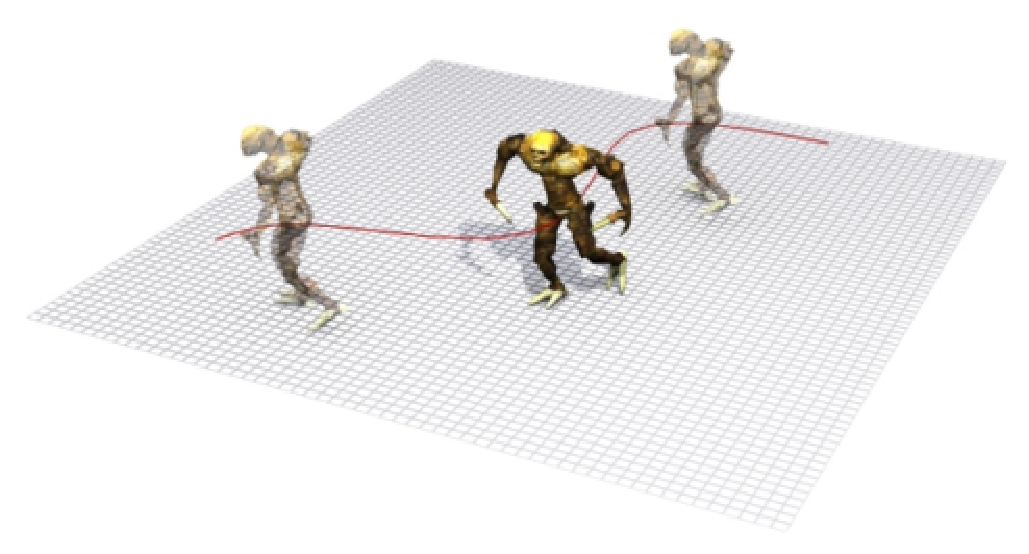
\includegraphics{pics/Paths.eps}
  \end{center}
  \caption{Actor walking on a path}
  \label{fig:Actor walking on a path}
\end{figure}

Paths can be build by hand or automatically as result of for instance a graph query. (path finding)



\subsubsection{Create Paths by Hand}
It's possible to build a path by hand during runtime. Call the graph path managers creation function \emph{GraphPathManager::Create()} to generate a new path. The function will return a pointer to the new path and now it's up to you to fill up this path with nodes.

New nodes are added using the path function \emph{GraphPath::AddNode()} which will take a path node as parameter. Note that this path node is just linked. The path node itself is in the simplest case only a world coordinate. \emph{GraphNode} also offers some tool functions like to compute the distance to another node using \emph{GetDistance()}.

Example:

\begin{lstlisting}[caption=Path creation example]
//	Test path:
//	  /B-------------C\
//	 /                 \
//	A                   D
//	 \                 /
//	  \F-------------E/

// Build path visualized above
GraphPath cPath;
GraphNode *pNode;

// A
pNode = new GraphNode("A");
cPath.AddNode(*pNode);
pNode->SetPos(0.0f, 0.0f, 2.0f);
// B
pNode = new GraphNode("B");
cPath.AddNode(*pNode);
pNode->SetPos(2.0f, 0.0f, 0.0f);
// C
pNode = new GraphNode("C");
cPath.AddNode(*pNode);
pNode->SetPos(16.0f, 0.0f, 0.0f);
// D
pNode = new GraphNode("D");
cPath.AddNode(*pNode);
pNode->SetPos(19.0f, 0.0f, 2.0f);
// E
pNode = new GraphNode("E");
cPath.AddNode(*pNode);
pNode->SetPos(16.0f, 0.0f, 4.0f);
// F
pNode = new GraphNode("F");
cPath.AddNode(*pNode);
pNode->SetPos(2.0f, 0.0f, 4.0f);

// The path should be closed
cPath.SetClosed(true);
\end{lstlisting}



\subsubsection{File Format}
PixelLight path files have the extension \emph{path}.

\cleardoublepage

\chapter{PLGraphics}


\paragraph{Motivation}
There are tons of image file formats and image libraries. Images are a fundamental feature of GUI and 3D rendering systems. Because they are that important, we decided to create \emph{PLGraphics} which is an image library that fulfils the requirements of PixelLight and integrates itself quite well into the whole framework. Beside the image features, other important feature are the color classes.




\section{External Dependences}
The core of PLGraphics depends on the \textbf{PLCore} and \textbf{PLMath} libraries. PLGraphics comes with some static linked image loader plugins so the library can directly load in several standard format. Some image loader plugins are using open source third party libraries which are static linked. As a result, the resulting PLGraphics library has no additional external third party shared library dependencies.


\paragraph{libjpeg}
\begin{itemize}
\item JPG image loading library
\item \emph{jpg} license
\item Version \emph{8b} (16-May-2010)
\item Used by the image loader plugin class \emph{ImageLoaderJPG}
\item Downloaded from \url{http://www.ijg.org/}
\end{itemize}


\paragraph{libpng}
\begin{itemize}
\item PNG image loading library
\item \emph{png} license
\item Version \emph{1.5.4}
\item Used by the image loader plugin class \emph{ImageLoaderPNG}
\item Downloaded from \url{http://www.libpng.org/}
\end{itemize}




% Include the other sections of the chapter
\section{Image}
Image data is frequently used in various forms within the PixelLight framework. GUI images, renderer textures and so on, all those are using the image class of PLGraphics to load in the data in one of the many supported image file formats or saving the data.

The image class may look quite complex on the first look, but using it is... now, look for yourself:

\begin{lstlisting}[caption=Image usage]
// Image instance
PLGraphics::Image cImage;

// Load an image
if (cImage.LoadByFilename("MyImage.png")) {
	// Get a pointer to the image buffer
	PLGraphics::ImageBuffer *pImageBuffer = cImage.GetBuffer();
	if (pImageBuffer && pImageBuffer->GetDataFormat() == PLGraphics::DataByte) {
		// Get a pointer to the image data
		PLCore::uint8 *pData = pImageBuffer->GetData();

		// Loop through the hole image data and mess it up
		for (PLCore::uint32 i=0; i<pImageBuffer->GetDataSize(); i++, pData++)
			*pData = ((*pData) + i) % 255;

		// Save the manipulated image
		cImage.SaveByFilename("MyManipulatedImage.png");
	}
}
\end{lstlisting}




\subsection{Mipmaps}
Mipmaps are the same image - but in multiple resolutions.\footnote{Although it's also possible to put a totally different image into each of the mipmaps}

Mipmaps are usually used for textures to improve the performance and the visual quality.
Within PLRenderer: If a texture is allowed to use mipmapping, mipmaps are created automatically if the loaded texture doesn't provide such information. Image formats like dds can provide predefined mipmap information. In this case, you have to define all mipmap levels down to 1x1 otherwise the texture is invalid when you try to use any min filter that uses mipmaps. OpenGL normally uses white color when invalid/incomplete texture is enabled.




\subsection{Compression}
The image system supports holding a compressed version of the image data. Supported compression formats are DXT1, DXT3, DXT5, ATI1N and ATI2N (marketing name: 3Dc).

The main usage is for texture compression. If a texture is allowed to use compression, the image is compressed by the renderer automatically if the loaded texture doesn't provide such information. Image formats like dds can provide compressed image information. In this case, the renderer will use this compressed data instead compressing automatically. Because the image system is only decompressing image data when really required, loading of compressed textures is quite fast!




\subsection{Cube Maps}
Cube maps are a special type of an image. In fact a cube map is build up of 6 different images - one for each cube side with the same dimensions. The cub map itself is used like the other normal images.

You can for example use the dds file format to load in cube maps.

The main usage is for textures. Cube textures are useful for
\begin{itemize}
\item{As a texture: Cube map reflections}
\item{As a texture: A normalization cube map can be used within fragment shaders to normalize vectors faster\footnote{But with less quality and on modern hardware it may not be faster}}
\end{itemize}




\subsection{3D Images}
Besides 2D images, the image system does also support 3D images. 3D images can be seen as a stack of 2D images.

The main usage is for textures. A 3D texture is mapped into (s, t, r = u, v, w = x, y, z) coordinates such that it's lower left back corner is (0 ,0, 0) and it's upper right front corner is (1, 1, 1).

\begin{figure}
  \begin{center}
    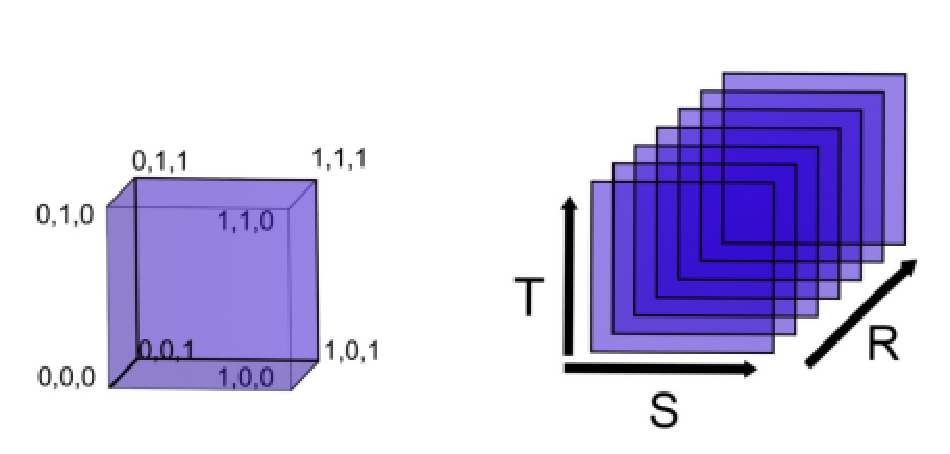
\includegraphics{pics/3DTex_1.eps}
  \end{center}
  \caption{3D texture}
  \label{fig:3D texture}
\end{figure}

3D textures are useful for

\begin{itemize}
\item{Volume rendering and examining a 3D volume one slice at a time}
\item{Animating textured geometry, for example, people that move}
\item{Eliminating distortion effects that occur when you try to map a 2D image onto 3D geometry}
\item{Solid texturing, for example, wood, marble and so on}
\end{itemize}

Texel values defined in a 3D coordinate system form a texture volume. You can extract textures from this volume by intersecting it with a plane oriented in 3D space, as shown below.

\begin{figure}
  \begin{center}
    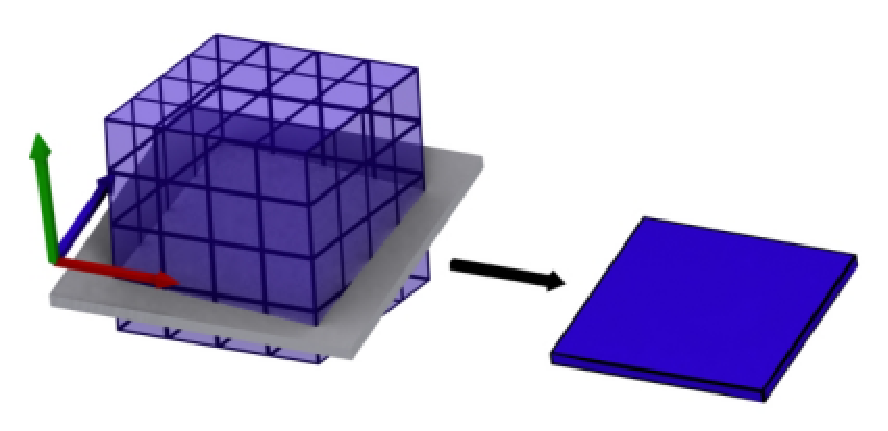
\includegraphics{pics/3DTex_2.eps}
  \end{center}
  \caption{3D texture}
  \label{fig:Extracting a Planar Texture From a 3D Texture Volume}
\end{figure}

The resulting texture, applied to a polygon, is the intersection of the volume and the plane. The orientation of the plane is determined from the texture coordinates of the vertices of the polygon.

\cleardoublepage

%----- Preamble ----------------------------------
\documentclass[a4paper,12pt]{book}
\usepackage[T1]{fontenc}
\usepackage[latin1]{inputenc}
\usepackage{color}
\usepackage{verbatim}
\usepackage{fancybox}
\usepackage[alsoload=binary, mode=text,loctolang={DE:german},decimalsymbol=comma]{siunitx}	% Units (bit, byte and so on)
\usepackage{../Common/Tools}
\usepackage{../Common/Styles}
\usepackage[dvipdfm]{graphicx}
\usepackage{textcomp}
\flushbottom

\sloppy	% Avoid writing over linebreak
\hbadness=10000
\clubpenalty = 10000 % schliesst Schusterjungen aus
\widowpenalty = 10000 % schliesst Hurenkinder aus

% Links
\usepackage[dvipdfm, colorlinks=true, urlcolor=black, linkcolor=black]{hyperref}
\urlstyle{same} % Use normal font for Urls
\usepackage[all]{hypcap} % Link to the image, not the image caption

% Table
\usepackage{tabularx}
\usepackage{threeparttablex}
\usepackage{booktabs}
\usepackage{ltxtable}

% Code listening
\usepackage{color,listings}
\definecolor{darkgreen}{rgb}{0,0.5,0}
\definecolor{lightgray}{gray}{0.95}
\lstset{language=C++,
captionpos=b,
frame=single,
basicstyle=\ttfamily,
keywordstyle=\color{blue},
commentstyle=\color{darkgreen},
stringstyle=\color{red},
backgroundcolor=\color{lightgray},
numbers=left,
numberstyle=\tiny,
numbersep=5pt,
breaklines=true,
showstringspaces=false,
columns=fullflexible,	% Please, don't change e.g. "export ANDROID_SDK=~/android-sdk-linux_x86" into "export ANDROID_SDK =~/ android -sdk - linux_x86"
tabsize=2,
emph={double,bool,int,unsigned,char,true,false,void},
emphstyle=\color{blue},
emph={Assert,Test},
emphstyle=\color{red},
emph={[2]\using,\#define,\#ifdef,\#endif}, emphstyle={[2]\color{blue}}
}
	% "input" instead of "include" is used to avoid problems with write permissions during TeX processing
\begin{document}


%----- Title -------------------------------------
%----- Title -------------------------------------
\thispagestyle{empty}
\begin{center}

{\Huge \textbf{PixelLight PLScene documentation}}\\
%----- Title -------------------------------------
\thispagestyle{empty}
\begin{center}

{\Huge \textbf{PixelLight PLScene documentation}}\\
\input{../Common/Title}

\end{center}


\end{center}

\tableofcontents


%----- Document ----------------------------------
\chapter{Introduction}


\paragraph{Motivation}
The PixelLight math component provides common required tools like vector and matrix classes and therefore implements features, which are especially useful when dealing this 3D graphics.




\section{External Dependences}
PLMath only depends on the \textbf{PLCore} library and doesn't use any external third party libraries.




\section{Transforming 2D to 3D and reversed}


\paragraph{Overview}
Sometimes it's required to project a 3D world position onto the screen to get the 2D x/y display position of it or you want to find out on which 3D world position a 2D position is on. This can be seen as the interface between the flat 2D screen and the 3D world.


\paragraph{3D to 2D}
\emph{Vector3::To2DCoordinate()} returns the 2D screen coordinate corresponding to a given 3D world coordinate using the given camera settings. This can be useful if you e.g. want to set the mouse cursor over a given 3D object.


\paragraph{2D to 3D}
\emph{Vector3::To3DCoordinate()} returns the 3D coordinate corresponding to a given 2D screen coordinate using the given camera settings. 2D to 3D transformation is extremely useful if you want to perform picking were the user is able to select a 3D object by using the mouse. Because picking is a collision task were we have to find the intersection point of the line (camera position to mouse position) and the meshes, this is not handled in this document. Have a look at the \emph{PixelLight API documentation} for more information how to perform picking.





\section{Additional tool functions}
\emph{PlaneSet::CreateSelectionPlanes()} takes a 2D start and end point and will return a plane set with the \emph{selection planes}. This plane set can be seen as \emph{selection frustum} and you can test your objects against it to see what's selected and what's not.

\chapter{General}




\section{Keep it Simple!}
The world is complicated enough - if there are multiple solutions, prefer the simplest over the most complicated one! This way, the chances are high that other will understand the solution as well as you when looking at the code some years later.




\section{Encoding}
We work with multiple operation systems so we have to take into account \emph{how} text files are saved. All \emph{Diary}, \emph{Readme}, \emph{Todo} and \emph{Plan} text files saved as "Unicode (UTF-8 with signature) - Codepage 65001". All other text files like code or make files saved in classic \emph{ANSI}.




\section{File Extension}
First of all, we use the old fashion \emph{.h}-file extension to mark header files - \emph{hpp} would be the \emph{correct} extension for C++, but it's not widely used. Usually, we outsource inline implementations into files with an \emph{inl}-extension to keep the header files good readable. For source codes, we use the file extension \emph{cpp}.




\section{C++11 Language Features}
Using C++11 (previously known as C++0x) language features is fine as long as
\begin{itemize}
\item{It's possible to emulate, or at least deactivate the feature within compilers don't supporting it (yet)}
\item{There's no comfortable/acceptable way to solve a task without using the feature, but those situations have to be discussed within the team and community}
\end{itemize}
\textsl{}
Currently the following C++11 language features are used:
\begin{itemize}
\item{\emph{nullptr} - a null pointer literal}
\item{\emph{override} - gives the compiler a chance to detect and blame errors related to overwriting methods}
\end{itemize}


\paragraph{Extern Templates}
Don't use \emph{extern templates}\footnote{\url{http://www2.research.att.com/~bs/C++0xFAQ.html\#extern-templates}} in order to avoid template instantiation in other modules. This is a feature we can't emulate and there are still legacy compilers like \ac{GCC} 4.2.1 used on Mac OS X 10.6 actively used around the world. So, at least for now, don't use this useful feature.




\section{For-Scope}
Within the PixelLight projects, the \emph{for-scope} is active by default. The following for instance will produce a compiler error:
\begin{lstlisting}[caption=for-scope]
for (int i=0; i<1; i++) {
	// Do anything
}
i = 20;	// i has already gone out of scope
\end{lstlisting}




\section{Null Pointer}
For null pointers, use \emph{nullptr}\footnote{For example \emph{Microsoft Visual Studio 2010} and \emph{\ac{GCC} 4.6} have native support for \emph{nullptr}} from \emph{C++11} and not for example the legacy, but traditional \emph{NULL} definition or even directly a integer $0$.

\begin{lstlisting}[caption=Null pointer]
char *pszMyString = nullptr;
\end{lstlisting}




\section{Overwriting Methods}
Put the methods within the base class, which are allowed to be overwritten, into a separate code block so everyone is able to find them at once.
\begin{lstlisting}[caption=Virtual methods within a base class]
//[-------------------------------------------------------]
//[ Public virtual MyClass functions                      ]
//[-------------------------------------------------------]
virtual void MyMethod() = 0;
\end{lstlisting}

When overwriting virtual methods within a derived class, put the overwritten methods into a code block telling were those methods originally came from.
\begin{lstlisting}[caption=Overwriting virtual methods within a derived class]
//[-------------------------------------------------------]
//[ Public virtual MyClass functions                      ]
//[-------------------------------------------------------]
virtual void MyMethod() override;
\end{lstlisting}
Although technically not required, do also add a \emph{virtual} to make it absolutely clear that this is a virtual method. To give the compiler a chance to find and blame possible errors like a signature change within the base class, use the C++11 language keyword \emph{override}.




\section{Casting}
PixelLight is using \emph{C++ style casts} (\emph{int i = static\_cast<int>(42.21f)}), not \emph{C style casts} (\emph{int i = (int)42.21f}). It's much easier to search for \emph{C++ style casts}\footnote{\emph{static\_cast}, \emph{reinterpret\_cast}, \emph{const\_cast}, and \emph{dynamic\_cast}} and they are less vulnerable to unintended effects as well - and because they are not that compact as the \emph{C style casts}, one may think about it a second time why there's a need for a cast.

\paragraph{\ac{GCC}}
\ac{GCC}, offers an option called \emph{-Wold-style-cast} to let the compiler warn if an old-style (C-style) cast to a non-void type is used within a C++ program.




\section{Const Correctness}
Define functions, variables etc. whenever possible to be constant. By giving the compiler this hint, it may be possible to use special optimizations or uncover bugs within the implementation.


\paragraph{Const Example}
Have a look at the following example function:
\begin{lstlisting}[caption=Non-constant function parameter]
void MyFunction(PLMath::Vector3 &vPosition)
{
	// ...
}
\end{lstlisting}
In case the function is considered to manipulate \emph{vPosition}, all's fine. Let's continue with another usage example:
\begin{lstlisting}[caption=Using a temporary variable instance as non-constant function parameter]
MyFunction(PLMath::Vector3(0.0f, 1.0f, 2.0f));
\end{lstlisting}
The compiler creates a temporary \emph{PLMath::Vector3} instance on the runtime stack and is passing a reference into the function. Looks fine as well? In case the function manipulates the variable passed by reference, the temporary instance is changed. In principle that's no problem because it's thrown away after the function call anyway. In practice, this situation is considered to be evil. \ac{MSVC} 2010 will shy tell you via a warning
\begin{quote}warning C4239: nonstandard extension used : 'argument' : conversion from 'PLMath::Vector3' to 'PLMath::Vector3 \&' A non-const reference may only be bound to an lvalue\end{quote}
So, it's possible to just ignore or even deactivate this warning... isn't it? In fact, it isn't because other compilers might not be that tollerant and will throw an error message at you. To sum this up: In the example above, you really want to write
\begin{lstlisting}[caption=Constant function parameter]
void MyFunction(const PLMath::Vector3 &vPosition)
{
	// ...
}
\end{lstlisting}
in order to be cross-platform safe.


\paragraph{Const Exception}
There's one situation were we do not use \emph{const} - when dealing with function parameters because

\begin{lstlisting}[caption=Function parameters]
void MyFunction(int nVariable1, int nVariable2);
\end{lstlisting}

is inside headers better readable than

\begin{lstlisting}[caption=Constant function parameters]
void MyFunction(const int nVariable1, const int nVariable2);
\end{lstlisting}

In this situation, the readability is more important for us. This rule does not apply for pointer or reference parameters like

\begin{lstlisting}[caption=Constant function pointer/reference parameter]
void MyFunction(const String &sVariable);
\end{lstlisting}

because the user should be able to see whether or not a function is going to manipulate the parameter variable!




\section{static const Vs. const static}
Use \emph{static const} instead of \emph{const static}. Have a look at e.g. the \ac{GCC} option \emph{Wold-style-declaration} resulting in the warning \begin{quote}`static' is not at beginning of declaration\end{quote} or into chapter 6.11 of ISO C99 (\emph{Future Language Directions} -> \emph{Storage-class specifiers}).




\section{Namespaces}
PixelLight is using multiple namespaces, one for each sub-project. If you want to use for instance the string class which is defined in \emph{PLCore} you need to do this:

\begin{lstlisting}[caption=Explicit namespace]
PLCore::String sMyString;
\end{lstlisting}

Or this:

\begin{lstlisting}[caption=Using namespace]
using namespace PLCore;
...
String sMyString;
\end{lstlisting}

Try to avoid using \emph{using namespace} too often or this will result in name conflicts which you then have to resolve by hand by adding for instance \emph{PLCore::}. We recommend to never use \emph{using namespace} within header files!




\section{Dynamic Parameters}
When dynamic parameters are used and the name of the parameters inside a string is irrelevant, as this is the case for \emph{PLCore::Params::FromString}, the parameters are named using \emph{Param<x>} were x starts with $0$ (example: \emph{Param0=1 Param1=''Hello''}).  




\section{Names}
In general, names of classes, functions, variables and so on must have human readable names. The name has to tell as much as possible about the usage - if the user can guess correctly the usage of for example a variable by just looking at it's name, the name is perfect.

General rules:

\begin{itemize}
\item A single character as name for local (only local!) control variables like \emph{i} within a for-loop is acceptable as long as there are not to much of those at once (else use reasonable names to avoid confusion!)
\item Short cuts should be avoided whenever possible because they may leads to confusion\footnote{True story: When using \emph{Rot} as short cut for \emph{Rotation}, we once had the situation that a German speaking programmer asked confused what the color \emph{Rot} should do inside the scene node... in German, \emph{Rot} is the word for \emph{red}...} (NO stuff like \emph{stricmp()}!)
\item If there's a \emph{commonly used} name for something, just this name instead of creating a totally new one
\item Avoid long names, if there's an expressive shorter name it's the preferred one... but keep the short cut rule in mind!
\end{itemize}

Classes, structures and so on have a upper case letter at the beginning. Example:

\begin{lstlisting}[caption=Name convention]
class Player {
};
struct Info {
};
\end{lstlisting}




\section{Prefix}
Because the readability of code is extremely important when working in a team and/or using code from others, one of our goals was to make the PixelLight code as readable and well structured as possible. We are using a name style convention\footnote{We know that there are a lot of discussions around the internet whether or not prefixes should be used. In the year 2002 we decided to use them and we don't change it - due to the dimension of the PixelLight project, it would be a huge effort to change it anyway.}.

Variable prefixes for standard types:

\begin{lstlisting}[caption=Variable prefixes for standard types]
Type               Prefix    Example
bool               b         bool bActive

(n for all none standard floating point types)
int                n         int  nNumber
char               n         char nCharacter
long               n         long nHuge

float              f
double             d

(Character arrays -> strings)
char[]             sz        char szName[64]
char*              psz       char *pszName

(Pointers)
*                  p         Player *pPlayer

(References)
&                  -         char &nTest = nTest2;

struct instance    s         Info sPlayer (struct Info)

class instance     c         Player cPlayer (class Player)
\end{lstlisting}

General variable prefix for class variables:
m\_ (m for member)\\
Example: char *m\_pszName\\

Variable prefixes for PixelLight types:

\begin{lstlisting}[caption=Variable prefixes for PixelLight types]
Type               Prefix    Example
String             s         String sName

Container          lst       List lstNames

Map                map       HashMap mapNames

VectorX            v         Vector3 vPosition
(X for dimension: 2, 3 or 4)

MatrixXxX          m         Matrix4x4 mRotation
(X for dimension: 3 or 4)

Quaternion         q         Quaternion qRotation

ColorX             c         Color3 cColor (same as class)
(X for dimension: 3 or 4)
\end{lstlisting}




\section{Postfix}
We recommend you to use the PixelLight name convention and marking debug versions with a \emph{D} at the end of the filename. Example: \emph{MyPlugins.dll} = release version, \emph{MyPluginsD.dll} = debug version.




\section{Events and Signals}
As soon as an event is inside a class, we refer to it as \emph{signal}. As such, the prefix \emph{Event} like within \emph{EventKeyDown} is used outside classes while prefix \emph{Signal} like within \emph{SignalKeyDown} is used inside classes.




\section{Event Handlers and Slots}
Within our name convention for event handlers and \ac{RTTI} slot names, there's a \emph{On} within for example \emph{OnMyEvent} indicating that this is a handler/slot method. The other part of the name consists of the name of the event/signal - for \emph{OnMyEvent} this would be an event/signal with the name \emph{MyEvent}.




\section{\ac{RTTI} Interface}
Within PixelLight, the \ac{RTTI} class properties and members are always defined in the following order:
\begin{itemize}
\item Properties
\item Attributes
\item Constructors
\item Methods
\item Signals
\item Slots
\end{itemize}
This way one knows exactly were to look for something. Further, within the \ac{RTTI} class properties and members definitions, only tabs and no spaces are used to make it easier to write the definitions like a table. This makes it more comfortable for the eyes and brain to navigate to certain definition parts without to much searching around.

Here's an example source code showing the common \ac{RTTI} interface layout (without the word wrap):
\begin{lstlisting}[caption=\ac{RTTI} interface (without the word wrap)]
//[-------------------------------------------------------]
//[ RTTI interface                                        ]
//[-------------------------------------------------------]
pl_class(pl_rtti_export, MyRTTIClass, "", PLCore::Object, "Sample RTTI class, don't take it to serious")
	// Properties
	pl_properties
		pl_property("MyProperty",	"This is a property value")
	pl_properties_end
	// Attributes
	pl_attribute(Name,	PLCore::String,	"Bob",	ReadWrite,	GetSet,			"A name, emits MySignal after the name was changed",			"")
	pl_attribute(Level,	int,			1,		ReadWrite,	DirectValue,	"Level, automatically increased on get/set name and OnMyEvent",	"")
	// Constructors
	pl_constructor_0(DefaultConstructor,	"Default constructor",	"")
	// Methods
	pl_method_0(Return42,			int,					"Returns 42",							"")
	pl_method_1(IgnoreTheParameter,	void,			float,	"Ignores the provided parameter",		"")
	pl_method_0(SaySomethingWise,	void,					"Says something wise",					"")
	pl_method_0(GetSelf,			MyRTTIClass*,			"Returns a pointer to this instance",	"")
	// Signals
	pl_signal_1(MySignal,	PLCore::String,	"My signal, automatically emitted after the name was changed",	"")
	// Slots
	pl_slot_0(OnMyEvent,	"My slot",	"")
pl_class_end
\end{lstlisting}



\section{Reuseability and adding new Stuff}
Before you add new classes, functions an so on - check first whether there's already something similar within PixelLight. If there's something you can already use directly, use it instead of writing new stuff. If there's something quite similar, have a more detailed look at it and contact your team colleagues to discuss whether a refactoring is possible and reasonable to update and/or to enhance existing stuff.

Reuseability is one of the most important concepts when creating frameworks like PixelLight... and reuseability does not mean that it's possible to copy'n'past it and then hacking around for a certain project! Reuseability means that it's possible to directly reuse, to share, something between multiple projects in a quite universal way without the need to enhance and hack around constantly!

\chapter{Renderer backends}
This chapter deals with the different renderer backends shipping with the PixelLight SDK.




\section{Null}
\begin{itemize}
\item The null renderer backend is for situations were you don't need \emph{real} rendering output. It consists of dummy functions which will try to \emph{emulate} the set \& get functions that good as possible.
\item PixelLight component name: PLRendererNull
\item Used dll's: \emph{PLRendererNull.dll}
\end{itemize}




\section{OpenGL}
\begin{itemize}
\item This is the preferred renderer backend of the PixelLight team because OpenGL\footnote{More information about OpenGL can be found at \url{http://www.opengl.org/}} provides some nice features like line width and it's also supported by other operation systems like Linux.
\item PixelLight component name: PLRendererOpenGL
\item Used dll's: \emph{PLRendererOpenGL.dll}
\item FreeType\footnote{FreeType can be downloaded from \url{http://www.freetype.org/}} is used for font support.
\end{itemize}

Here's a list of some general notes:
\begin{itemize}
\item Normally when using rectangle textures (none power of 2) under OpenGL, you have to work with none normalized texture coordinates - but because we don't want to deal with texture coordinates for rectangle textures in a special way, within the backend the texture matrix is scaled. So, you always work with normalized texture coordinates. But if you use rectangle textures within a shader, you should take the texture matrix within your vertex shader into account!
\end{itemize}

There's a plugin for PLRendererOpenGL adding support for the Cg\footnote{(\url{http://developer.nvidia.com/object/cg_toolkit.html})} shader language:
\begin{itemize}
\item PixelLight component name: PLRendererOpenGLCg
\item Used dll's: \emph{PLRendererOpenGLCg.dll}, \emph{cg.dll} and \emph{cgGL.dll}
\end{itemize}




\section{OpenGL ES 2.0}
\begin{itemize}
\item Currently not within the official PixelLight SDK
\item OpenGL ES 2.0 renderer backend for mobile devices
\item PixelLight component name: PLRendererOpenGLES
\item FreeType\footnote{FreeType can be downloaded from \url{http://www.freetype.org/}} used for font support.
\end{itemize}




\section{Direct3D 9}
\begin{itemize}
\item Currently not within the official PixelLight SDK
\item This Direct3D 9\footnote{For more Direct3D information, please have a look at \url{http://www.microsoft.com/downloads/Browse.aspx?displaylang=de&categoryid=2}} renderer backend is for \emph{Microsoft Windows} systems only, and has some missing features.
\item PixelLight component name: PLRendererD3D9
\item Used dll's: \emph{PLRendererD3D9.dll}, \emph{cg.dll} and \emph{cgD3D9.dll} and DirectX 9 must be installed
\end{itemize}

Here's a list of some general notes:
\begin{itemize}
\item No line width support. \emph{SetLineWidth()} has no effect and \emph{GetLineWidth()} will always return 1
\item Because D3D doesn't have any constant color, \emph{SetColor()} must be emulated within this backend using for instance a vertex shader
\end{itemize}
Further, within this backend there are still some bugs to fix.




\section{Direct3D 11}
\begin{itemize}
\item Currently not within the official PixelLight SDK, project is quite new and heavily under construction
\item This Direct3D 11\footnote{For more Direct3D information, please have a look at \url{http://www.microsoft.com/downloads/Browse.aspx?displaylang=de&categoryid=2}} renderer backend is for \emph{Microsoft Windows} systems only, and has some missing features.
\item Windows Vista and Windows 7 only
\item PixelLight component name: PLRendererD3D11
\item Used dll's: \emph{PLRendererD3D11.dll} and DirectX 11 must be installed
\end{itemize}

%----- Chapter: High level: Textures --------------
\chapter{High level: Textures}


[TODO] Update!


%----- Section: Overview -------------------------
\section{Overview}
Because the materials normally using textures it's good to know some hinds about it - read this
section carefully!
There are different types of textures like 1D, 2D, \hyperlink{Rectangle textures}{rectangle textures},
\hyperlink{3D textures}{3D}), \hyperlink{Cube maps}{cube map textures}) etc.




%----- Section: Texture formats ------------------
\section{Texture formats}
PixelLight can load the following texture formats:\\

bmp, cut, ico, jpg, pcx, tif, png, tga, dds, psd, hdr, exr\\

and save this formats:\\

bmp, jpg, pcx, png, pnm, raw, sgi, tga, tif, pal, hdr, exr\\

If you don't specify the texture format by the filename extension the framework will search for the
texture by adding a filename extension in the order you could see above. PixelLight has no own texture format
because this would be to complex to the graphical artists to convert the textures to a special format.
Normally textures etc. are packed in a zip file and the user will not see them.

Beside the texture files like bmp, tga, jpg etc. which store the texture data itself there are
several additional PixelLight texture description file formats. This PixelLight texture file formats are described below in
detail, here were we only want to mention them in order to let you know that they exist and how to
use them.\\
Each texture file (bmp, tga etc.) can have additional PixelLight relevant information which are defined
in a plt-file with the same texture filename but with the filename ending 'plt' e.g. 'MyTexture.bmp'
would have a 'MyTexture.plt' plt-file which is in the same directory as the owner texture. In this
additional texture file you are able to setup different fixed properties for this texture like if
the texture can be scaled, if GPU texture compression is allowed, the color key for alpha transparency
etc. (such a color key can also be defined in a tga RGBA texture)\\
In the \hyperlink{tani}{tani-format} format you can define texture animations like sliding/rolling
texturs, texture animations through different texture frames etc. Such tani-files can be loaded by
texture handlers and materials as all other texturs, too.

It's recommended to use dds textures with precalculated mipmaps and compression whenever possible
for better loading performance.




%----- Section: PixelLight texture format (plt) --
\section{PixelLight texture format (plt)}
In the plt-format files which have the same name as the 'real' texture (bmp, jpg etc) with the texture
data itself but with the ending 'plt' you can setup some different fixed texture properties like its
color key for alpha masking, whether texture compression is allowed or not etc. This texture
configuration file is a normal text file you can edit with every text editor. Unrequired commands
can be skipped - in this case standard values will be used instead.

First here's a full plt-format example with the standard values:\\
\verbatiminput{examples/example.plt}


General texture configurations\\

\begin{tabular}{|p{2.5cm}|p{2.5cm}|p{9cm}|}
\hline
\textbf{Command} & \textbf{Default} & \textbf{Description}\\
\hline
CubeMap & 0 &
\begin{tabular}{|p{9.5cm}|}
\hline
Is this a cube map?
If yes the other 5 textures will be loaded automatically using the texture name + ID\\

\begin{tabular}{|p{3cm}|p{2.5cm}|}
\hline
\textbf{Side} & \textbf{Index}\\
\hline
positive x & -\\
negative x & 1\\
positive y & 2\\
negative y & 3\\
positive z & 4\\
negative z & 5\\
\hline
\end{tabular}

Example:\\
Sky.tga (this texture you load)\\
Sky1.tga Sky2.tga Sky3.tga Sky4.tga Sky5.tga (loaded automatically)\\
\end{tabular}\\

\hline
Mipmaps		& config & Are mipmaps allowed?\\
\hline
Compression	& config & Is texture compression allowed? (less quality but better performance) Do not use standard texture 
                       compression for normal maps, because this textures stores vector data instead of visible colors 
                       the result would be wrong. If for instance the loaded dds texture is already compressed by
                       default, this compression option is ignored because it would be pretty useless to uncompress
                       this texture before uploading to the GPU... there's already a loss of quality.\\
\hline
Gamma		& 1.0	 & Gamma factor\\
\hline
FitLower	& ?		 & Specifies the automatic texture scale behaviour.
					   If not defined, the texture manager settings will be used. If 1
					   the next valid lower texture size is used, if 0 the next higher one.\\
\hline
Rectangle	& 0		 & If 1 there's no power of 2 limitation for the texture size. If 0, the texture will normally be
                       resized automatically to a valid dimension. If rectangle textures are not supported by the GPU,
                       this settings is ignored and the texture is resized automatically.
 \\
\hline
\end{tabular}


Texture resize settings\\

\begin{tabular}{|p{2.5cm}|p{2.5cm}|p{9cm}|}
\hline
\textbf{Command} & \textbf{Default} & \textbf{Description}\\
\hline
Active	  & 1 & Can the texture size be resized to reduce the texture quality? If the texture dimension
                is not correct and the GPU can't use the texture without resizing it this is internally
                always set to true. Use the 'force' settings below to force a given size even if the GPU
                can't handle it.\\
\hline
MinWidth  & 4 & The minimum allow texture width (should normally be a power of 2!)\\
\hline
MinHeight & 4 & The minimum allow texture height (should normally be a power of 2!)\\
\hline
MinDepth  & 1 & The minimum allow texture depth (should normally be a power of 2!)\\
\hline
\end{tabular}


Forces a special static texture size if not -1. (texture resizing will be disabled!)\\
Use this only in special situations because the GPU may not be able to handle certain
sizes...

\begin{tabular}{|p{2.5cm}|p{2.5cm}|p{9cm}|}
\hline
\textbf{Command} & \textbf{Default} & \textbf{Description}\\
\hline
Width  & -1 & Forced texture width (should normally be a power of 2!)\\
\hline
Height & -1 & Forced texture height (should normally be a power of 2!)\\
\hline
Depth  & -1 & Forced texture depth (should normally be a power of 2!)\\
\hline
\end{tabular}


The color key defines the color which should be transparent.
You can also use a RGBA texture like a tga to create semi transparent textures, in that
case this RGB settings are not used! But note that in this case the material pass using this
RGBA texture in the first layer must have an active alpha test to use the alpha mask - else
you won't see any difference!\\

\begin{tabular}{|p{2.5cm}|p{2.5cm}|p{9cm}|}
\hline
\textbf{Command} & \textbf{Default} & \textbf{Description}\\
\hline
R		  & 0 & Red component (0-255)\\
\hline
G		  & 0 & Green component (0-255)\\
\hline
B		  & 0 & Blue component (0-255)\\
\hline
Tolerance & 0 & Alpha color tolerance value (0-128)\\
\hline
\end{tabular}



%----- Section: Texture handler ------------------
\section{Texture handler}
When working with textures you will use texture handler in your code. (PLTTextureHandler)\\
They will manage the basic texture stuff for you like loading them or set the correct texture states
like the wrapping functions. The texture handler will offer you an interface to work with the used texture.
The texture handlers are also responsible for texture animations like changing textures or rotation, move etc.
ones. Such texture animations you can create within your application by programming it directly
or through the PixelLight \hyperlink{tani}{tani-format} which are load by and dealed the texture
handlers like 'normal' texture, too.
The different material layers are implemented using such texture handlers.




%----- Section: Texture animation format (tani) --
\section{Texture animation format (tani)}
\hypertarget{tani}{}
With the texture animation configuration (normal ini text file) you can create animated textures.
There are three texture animation types:
\begin{description}
\item[Texture animations:] Animation through texture changing
\item[Matrix animations:]  Animation through texture transformation matrix manipulation
\item[Color animations:]   Animation through color changing
\end{description}
Unrequired commands can be skipped - standard values will then be used.\\

Heres a full texture animation example:\\
\verbatiminput{examples/example.tani}


Texture frame definitions\\
\\
\textbf{Frame:}\\
\\
Texture resize settings\\
\\
\begin{tabular}{|p{2.5cm}|p{2.5cm}|p{9cm}|}
\hline
\textbf{Command} & \textbf{Default} & \textbf{Description}\\
\hline
Texture & - & Texture filename of for this frame\\
\hline
\end{tabular}


Matrix frame definitions\\

\textbf{Frame:}\\

\begin{tabular}{|p{2.5cm}|p{2.5cm}|p{9cm}|}
\hline
\textbf{Command} & \textbf{Default} & \textbf{Description}\\
\hline
Pos   & 0.0 0.0 0.0 & Texture position\\
\hline
Scale & 1.0 1.0 1.0 & Texture scale\\
\hline
Rot   & 0.0 0.0 0.0 & Texture rot\\
\hline
\end{tabular}


Color frame definitions\\

\textbf{Frame:}\\

\begin{tabular}{|p{2.5cm}|p{2.5cm}|p{9cm}|}
\hline
\textbf{Command} & \textbf{Default} & \textbf{Description}\\
\hline
Color & 1.0 1.0 1.0 1.0 & Texture color (RGBA)\\
\hline
\end{tabular}


Animation definitions\\

There's always a texture, matrix and color animation with all frames by default.
The first animation of each type is played automatically after loading!\\

\begin{tabular}{|p{2.5cm}|p{2.5cm}|p{9cm}|}
\hline
\textbf{Command} & \textbf{Default} & \textbf{Description}\\
\hline
Type      & TEXTURE & Animation type
\begin{tabular}{p{3cm}p{6cm}}
Texture & Texture animation\\
\hline
Matrix  & Matrix animation\\
\hline
Color   & Color animation\\
\end{tabular}\\
\hline
Name      & -       & Animation name\\
\hline
Start     & 0       & Start frame\\
\hline
End       & 0       & End frame\\
\hline
Speed     & 1.0     & Animation speed (higher = faster)\\
\hline
Loop      & 1       & Loop animation?\\
\hline
Ping pong & 0       & Ping pong animation?\\
\hline
\end{tabular}


Frame settings\\

\begin{tabular}{|p{2.5cm}|p{2.5cm}|p{9cm}|}
\hline
\textbf{Command} & \textbf{Default} & \textbf{Description}\\
\hline
ID    & 0   & Frame ID\\
\hline
Speed & 0.0 & Speed of this frame (higher value = faster animation)\\
              &&  0.0 = Set value and skip this frame\\
              && < 0.0 = No interpolation\\
\hline
\end{tabular}


Event settings\\

\begin{tabular}{|p{2.5cm}|p{2.5cm}|p{9cm}|}
\hline
\textbf{Command} & \textbf{Default} & \textbf{Description}\\
\hline
FrameID & 0 &
If this frame is reached in the animation the event ID message is send to the entity connected
with the animation. You could use it e.g. to mark frames were a sound should be played.\\
\hline
ID      & 0 & Event ID\\
\hline
\end{tabular}




%----- Section: Procedural textures --------------
\section{Procedural textures}
Prodecural textures are textures which will be created and possibly updated during runtime.
Normally it's usefull to implement them as scene node which controls the procedural texture. Here's
an example how such an procedural texture entity might look:\\

\begin{lstlisting}[caption=Procedural texture class]
class SNProceduralTexture : public PLTSceneNode {
	...
	private:
		float m_fTimer;             // Timer

		// Exported variables
		char  m_szTextureName[64];  // Name of the texture
		int   m_nWidth;             // Texture width
		int   m_nHeight;            // Texture height
		float m_fSpeed;             // Animation speed

	private:
		virtual void InitFunction();
		virtual void DeInitFunction();
		virtual void UpdateFunction();
	...
};

void SNProceduralTexture::InitFunction()
{
	// Init data
	m_fTimer = 0.f;

	// Create texture
	PLTTextureManager::GetInstance()->CreateTexture(m_szTextureName, m_nWidth, m_nHeight);
}

void SNProceduralTexture::DeInitFunction()
{
	PLTTextureManager::GetInstance()->Unload(PLTTextureManager::GetInstance()->Get(m_szTextureName));
}

void SNProceduralTexture::UpdateFunction()
{
	// Animation speed
	m_fTimer += PLTTimer::GetInstance()->GetTimeDifference()*m_fSpeed;
	if (m_fTimer < 1.f) return;
	m_fTimer = 0.f;

	// Create texture
	PLTTexture *pTex = PLTTextureManager::GetInstance()->Get(m_szTextureName);
	if (!pTex) return;
	unsigned char *pData = pTex->GetData();
	if (!pData) return;
	for (int i=0; i<pTex->GetWidth()*pTex->GetHeight(); i++) {
		*pData = *(pData+1) = *(pData+2) = PL::Math.GetRand() % 255;
		pData += 3;
	}

	// Upload new texture
	pTex->Upload();
}
\end{lstlisting}

This example creates a new texture using the texture manager function CreateTexture(). Then from
time to time the texture data is filled up with random color values and is finally uploaded to the GPU.
This would result in a dynamic random noise texture. Dynamic created textures are used like all other normal
textures. E.g. you can load them in a texture handler using Load("Texturename"). But note that
this texture must already exist before you are able load them in a texture handler or material else
this texture will be unknown!\\
In this way you can also create special textures you e.g. need for your shaders. For instance
if you need a normalization cube map you implement an scene node which will create this texture for you
so that you can use it in the materials like all other textures, too! But note that this textures
must be created BEFORE a material is loading them! This is an intuitive way to deal with self calculated
textures without to be forced to handle such textures in a special manner.



%----- Section: Alpha test -----------------------
\section{Alpha test}
Alpha test is one operation in the per-fragment operations stage of the renderer pipeline that
allows any further processing of the fragment to be aborted based on the value of its alpha component. The
fragment's alpha component is compared with an application-specified reference value
using an application-specified comparison function. If the fragment passes the test, it will
be processed by the subsequent fragment operation, otherwise it will be discarded. Alpha
test does not incur any extra overhead even if all the fragments pass the test. Unlike
stencil testing, depth testing, texturing, and blending, alpha testing do not involve
fetching data from memories external to the GPU. Alpha test is only available in RGBA
mode for instance when using tga textures with an alpha channel. You can setup the alpha
test withing the render state section, either directly by hand in the renderer (for programmers)
or in the render state section of a material technique pass. (see the material format in another chapter)

Alpha test provides a great way to save fill rate. When used to draw alpha blended
textures, or to do additive blending in multi-pass, it provides a means to reject the
fragment as early as possible in order to reduce the memory traffic due to stencil, depth,
and color buffer reads and writes.
Consider the case when an application draws big triangles on the screen, like lens
flares or explosions, and those triangles are transparent or blended with additive blending.
Additionally, consider the case of multi-pass rendering, which is common practice to
"shade" models and significantly increases the depth complexity. Typically, one can
render one pass to apply a textured diffuse lighting to a model, render another pass for the
specular highlight. In this second pass, an enormous number of fragments are just black,
due to the nature of the specular computation. We will demonstrate a technique, which
can optimize the application in such situation by mixing the use of alpha test and shaders,
in order to discard the black fragments.
Graphic programmers should reduce the overhead, caused by such rendering
architectures or effects, by utilizing fill rate saving techniques such as alpha test and
other tricks derived from specific hardware functionalities that can take advantage of
alpha test.

Here's a more advanced example when the alpha test can be quite useful to discard the black fragments
when dealing with range-limited lights and shaders:\\
Whenever a fragment is outside the range of the light, you can skip all the lighting math and just return
zero immediately. With pixel shader 3.0 you'd simply implement this with an if-statement. Without pixel
shader 3.0, you just move this check to another shader. This shader returns a truth value to alpha. The
alpha test then kills all unlit fragments. Surviving fragments will write 1 to stencil. In the next pass
you simply draw lighting as usual. The stencil test will remove any fragments that aren't tagged as lit.
If the hardware performs the stencil test prior to shading you will save a lot of shading power. In fact,
the shading workload is reduced to the same level of pixel shader 3.0, or in some cases even slightly below
since the alpha test can do a compare that otherwise would have to be performed in the shader. 
The result is that early-out speeds things up considerably. In theory you are able to to this completely within
the PixelLight material! Imagine a material with two techniques the more advanced one is using pixel shader 3.0 to ignore
unrequired fragments and if this fragment profile isn't available an alternative technique is used with two
passes: The first which will use the alpha test, stencil buffer and a special 'if' shader and the second one drawing
the stuff were it passes the stencil buffer which was set by the pass before.

By tuning appropriately the reference value of alpha test to reject the transparent or almost transparent
fragments, one can improve the application performance significantly. Basically, varying the reference value
acts like a threshold setting up how many fragments are going to be evicted. The more fragments
are being discarded, the faster the application will run. On the other hand, the more
fragment are being discarded, the more texture subtleties are not being drawn, potentially
leading to some undesirable visual side effects. In this particular case, it is crucial to take
into consideration the visual artifacts introduced by setting a reference value threshold
too aggressively. Therefore, setting up alpha test's reference value shouldn't be done
without taking the final visual quality into account.
Because using alpha test can speed up your application, one should consider adding an
explicit alpha channel to textures that are used in a way that burns a lot of fill rate and
that have areas that are not used.
	%[TODO] Update!
%%----- Chapter: High level: Shaders --------------
\chapter{High level: Shaders}


[TODO] Update!



%----- Section: Overview -------------------------
\section{Overview}
In general PixelLight is using the Cg shader language for vertex and fragment shader effects. Have 
a look at e.g. \url{http://www.shadertech.com/} or developer.nvidia.com/cg to learn the basics
about this technology. Because Cg is API and platform independent you can work with Cg functions
directly - therefore have a look at the Cg documentation to see how to use the Cg functions.\\
The PixelLight material is encapsulating this shaders and you haven't to work with them directly. But
because you can do alot with shaders you have also low level access to the shaders to be able
to create e.g. grass effects etc.\\

Vertex/fragment programs will process every vertices/fragments on the GPU. When using such programs
you normally will only work with the provided program parameters. The PixelLight shader system will give the
programmer the ability to use this shaders in the application.\\
The PixelLight shader handler PLTShaderHandler provides an interface with all required functions to work with
such programs. Each individual program needs it's own derived shader handler because each program has
different parameters and functionality! So, if you want to use a certain vertex/fragment program you
have to use it through its own shader handler. The shader handler is the obverse of the program on the GPU.




%----- Section: Shader handler -------------------
\section{Shader handler}
The main shader handler functions are Load(), Bind() and Update(). First you have to load up such
a vertex/fragment program using the Load() function of the shader handler. If the program filename
ends with a '+' it's a fragment program, else a vertex program. The filename ending of the programs
is '.cg'.\\
Then you should update the shader hander each frame to ensure that the internal parameters are
updated correctly. Before rendering anything the shader is activated using the Bind() function and
after the render process is finished it should be deactivated using Unbind().\\
Note that only one vertex and one fragment program can be active at the same time!\\
In the example below two derived shader handlers are used:\\

\begin{lstlisting}[caption=Using shader handler]
// Somewere in e.g. your class
TVertexShaderHandler   m_cVertexShader;
TFragmentShaderHandler m_cFragmentShader;

// Load somewere the vertex and fragment programs
  m_cVertexShader.Load("myVertexShader");
m_cFragmentShader.Load("myFragmentShader+");

// Render process
// Bind shaders
m_cVertexShader.Bind();
m_cFragmentShader.Bind();

// Draw anything

// Unbind shaders
m_cFragmentShader.Unbind();
m_cVertexShader.Unbind();

// Somewere in your code...
// Update shader handlers
m_cFragmentShader.Update();
m_cVertexShader.Update();
\end{lstlisting}




%----- Section: Derive shader handler ------------
\section{Derive shader handler}
To be able to use your own program you have to derive PLTShaderHandler to implement your shader
handler which will manage this the program.\\
After a program was loaded the virtual function CustomLoad() is called. There you should initialize
your handler and getting the program parameters. If the shader handler is bind the function CustomBind()
is called were the program parameters should be set. Finally use CustomUpdate() to update your shader
handler. Example:\\

\begin{lstlisting}[caption=Creating own shader handler]
class TVertexShaderHandler : public PLTShaderHandler {

    // Private data
    private:
        float m_fTime;

    // Programm parameters
    private:
        CGparameter m_ConstantsParam;
        CGparameter m_ModelViewProjParam;
        CGparameter m_ModelViewITParam;
        CGparameter m_ModelViewParam;

    // Virtual PLTShaderHandler functions
    private:
        virtual void CustomLoad();
        virtual void CustomBind();
        virtual void CustomUpdate();


};

void TVertexShaderHandler::CustomLoad()
{
    // Init data
    m_fTime = 0.f;

    // Get program variables
    m_ConstantsParam     = GetCGNamedParameter("Constants");
    m_ModelViewProjParam = GetCGNamedParameter("ModelViewProj");
    m_ModelViewITParam   = GetCGNamedParameter("ModelViewIT");
    m_ModelViewParam     = GetCGNamedParameter("ModelView");
}

void TShaderGrass::CustomBind()
{
    // Set program parameters
             cgGLSetParameter4f(m_ConstantsParam,     m_fTime, 0, 0, 1);
    cgGLSetStateMatrixParameter(m_ModelViewProjParam, CG_GL_MODELVIEW_PROJECTION_MATRIX, CG_GL_MATRIX_IDENTITY);
    cgGLSetStateMatrixParameter(m_ModelViewITParam,   CG_GL_MODELVIEW_MATRIX,            CG_GL_MATRIX_INVERSE_TRANSPOSE);
    cgGLSetStateMatrixParameter(m_ModelViewParam,     CG_GL_MODELVIEW_MATRIX,            CG_GL_MATRIX_IDENTITY);
}

void TShaderGrass::CustomUpdate()
{
    // Update timer
    m_fTime += PL::Timer.GetTimeDifference();
}
\end{lstlisting}




%----- Section: Material shader effects ----------
\section{Material shader effects}
In the shader section above you saw how to use shader effects as programmer directly in your program
by programming their usage by hand for special situations like grass effects were you also have to
create and setup the vertices in the correct way.
Because the vertex/fragment programs are extreme implementation dependent and the programer has to
do the most work graphic artists haven't that many control over them and new shader effects can't be
used without write some new code in your application - except the new effect is using the same parameters
etc. as another effect.\\
Therefore PixelLight has an advanced effect system which is implemented in the material itself to give the
graphic artists more control over the appearance of  surfaces etc - but in reverse the programmer
itself has less control because he isn't able to manipulate this cg programs directly in his code.\\




%----- Section: CgFX -----------------------------
\section{CgFX}
During development graphic artists can use CgFX which also provides the environment the vertex/fragment
programs will work in and is setting its own render states, used textures etc. Further the fx files
provide in contrast to cg files also a description of the program parameters with default values, gui
definitions in annotations to manipulare this values in editors using gui elements etc.
Also different techniques/fallbacks can be defined. The 'fx' file format is nealy the same as the
DirectX effect format and if you write your own programs in there it is identical to Cg or assembly
programs. There are plugins for \emph{Autodesk 3ds Max} etc which enables the graphic artists to develop the
advanced shader effects directly in their well kown development environment! The CgFX 'fx' file format
can be compared with the PixelLight own material file format 'mat', therefore is isn't that difficult to 
convert such CgFX effects artists had developed in their own development environment into the
PixelLight own material format.\\

PixelLight itself doesn't supply direct CgFX support because it doesn't provide a nice programmer
interface and is setting render states etc. automatically without enabling the programmer to find
out what in fact was set. Further CgFX isn't THAT compatible to other graphic cards (e.g. ATI) like
Cg itself which would result in many troubles. Therefore we decided to don't implementet CgFX directly
- but as mentioned above, the PixelLight own material format has nearly the same capability as CgFX
without the compatibility troubles CgFX has!\\

The material itself which can contain shaders is nearly used in the same way as the 'by hand' Cg shaders
are used. But unlike the direct shader interface the material effects provides a more comfortable
parameter interface. Further there are different known parameter semantics which will setup the
shader parameter automatically. (e.g. set current projection matrix) Therefore you mustn't derive
the PLTMaterial to deal with the different shader parameters. Some parameters with kown semantic
will be managed complete automatically and the other you can manipulate in a quite comfortable way
over the interface of the material.\\




%----- Section: Material shader parameters -------
\section{Material shader parameters}
The material shader parameters are split up into two parameter types:\\
- Parameter: Parameters were the semantic is unknown.
             They can be manipulated by hand.\\
- Semantic:  Parameters were the semantic is known.
             They will be updated automatically and shouldn't be manipulated
             by hand.\\




%----- Section: Parameter semantic ---------------
\section{Parameter semantic}
Here's a list of all known parameter semantic:\\

 \begin{tabular}{|p{7cm}|p{7cm}|}
\hline
\textbf{Parameter semantic} & \textbf{Description}\\
\hline
World               & World matrix (float4x4)\\
\hline
WorldI	            & World inverse matrix (float4x4)\\
\hline
WorldIT	            & World inverse transpose matrix (float4x4)\\
\hline
WorldView           & World view matrix (float4x4)\\
\hline
WorldViewI          & World view inverse matrix (float4x4)\\
\hline
WorldViewIT         & World view inverse transpose matrix (float4x4)\\
\hline
WorldViewProjection & World view projection matrix (float4x4)\\
\hline
Projection	        & Projection matrix (float4x4)\\
\hline
View	            & View matrix (float4x4)\\
\hline
ViewIT	            & View inverse transpose matrix (float4x4)\\
\hline
EyePos	            & Eye position (object space, float4)\\
\hline
EyeVector           & Eye direction vector (object space, float3)\\
\hline
EyePosWorld	        & Eye position (world space, float4)\\
\hline
EyeVectorWorld      & Eye direction vector (world space, float3)\\
\hline
Time	            & Timer (float)\\
\hline
Shininess	        & Shininess (float)\\
\hline
Color	            & Color (float4)\\
\hline
AmbientColor        & Ambient color (float4)\\
\hline
DiffuseColor        & Diffuse color (float4)\\
\hline
SpecularColor       & Specular color (float4)\\
\hline
EmissionColor       & Emission color (float4)\\
\hline
Texture<n>          & Texture 0-7 (texture)\\
\hline
TextureMatrix<n>    & Texture matrix 0-7\\
\hline
\end{tabular}
	%[TODO] Update!
%%----- Chapter: High level: Effects --------------
\chapter{High level: Effects}


[TODO] Update!


%----- Section: Overview -------------------------
\section{Overview}
In this section we will explain you how to use the PixelLight material in practice. A material 
is a simple text format which describes the settings of a material - skipped things are set to
default automatically. A text editor is enough to develop materials but theres also a materal
editor provided.



%----- Section: Introduction ---------------------
\section{Introduction}
Advanced material effects which will increase the visual quality of the surfaces is a must have
for modern graphics engines. Therefore PixelLight provides an extensive material system which enables you
to use the capabilities of modern GPU's to create amazing visual effects.\\

This PixelLight material guide will teach you what in detail such a material is, how to use and
build it - further some background information about e.g. what a 3D texture is are provided, but for
detailed information you have to use other documents you can for instance find in the internet. This document
is for both programmers and graphic artists because a material is a complex
and powerful surface description and it's also possible to programm byself advanced shaders to
control how each vertex and fragment is processed by GPU. In this section we will tell you some
backgrounds about the materials to give you an overview over this topic. In section 2 we will talk
about textures because this is the base of the materials. You will learn in section 3 how to use
materials in practice. Section 4 consists of a material format description. In the section
5 we will talk about shaders. Section 6 is a faq.\\

A PixelLight material is a powerfull surface description. It will manage the different render techniques
automatically (also called 'fallbacks') for you so that in fact you don't need to know which technique is
currently used to visualize a surface. Just apply a material to a surface and have fun! ;-)\\
Here's a diagram which shows how the PixelLight material is build up in general:\\

\begin{lstlisting}[caption=PixelLight material system overview]
                  material
                     |
          n techniques per material
                     |
            n passes per technique
                     |
           ----------------------
           |                    |
  n layers per pass      one vertex/fragment shader per pass
\end{lstlisting}

Techniques means that there are different ways how the material can be rendered - in this relation we 
also call this an 'effect'. If you are already familar with e.g. the Direct3D effect file format (fx) it will be
easy for you to understand the PixelLight material. Using advanced effects is an important thing because there
are fallbacks which enables you to use a simpler technique if the hardware or performance is insufficient or for 
material LOD. Such a technique can consist of different render passes which means that the material is rendered 
several times with different settings increasing the visual quality. In such a pass, render states, sampler states 
etc. are set to render the surface in the requested way.
Many render passes per material will reduce the performance because the geometrie the material
is applied to have to be drawn multiple times - so use it wise. Each of such a pass can have that
many texture layers the hardware is supporting. Modern graphic cards normally support 4 direct texture
layers and up to 16 and more layers when using shaders accessing this layers. Using such layers you can
blend together different textures without be forced to redraw the geometry which will blow up the
polycount and reduce problems like z-fighting. Further each layer can have another texture with other properties... 
you can also animate each textur using different changing subtextures to create a cartoon like animation or rotate, 
move etc the texture by changing it's texture matrix or using all this texture animation effects at the SAME TIME
to create amazing materials full of life! :)\\

An advanced material rendering control is supplied through the vertex and fragment shader you can apply
to each pass. A shader is a program running on the GPU. It will 'overwrite' the API (e.g. OpenGL)
fixpass functions which normally process vertices (transformations etc.) and fragments. (get the color
of each fragment etc.) Therefore when using a vertex shader you have to transform the vertices by self
or when using a fragment shader calculating the single fragment colors by hand. In this case the
different pass layers will only feed the active shaders with e.g. the desired textures but not combining
different texture layers automatically. Further you have to consider things like texture matrix animations
in your shaders when you want to use it - in contrast to the fixpass some things don't done automatically!
Note that per pass there's only ONE vertex and ONE fragment active shader! But for instance you can
combine different passes to a final result. It's a lot of work to write such materials with individual
shader effects but therefore you have FULL CONTROL over how it is rendered and you can create impressive
and unique material effects! If it is too much work for you to do all by self you can use the 'standard'
fixpass functions which which will also product good results in less development time - but you haven't
the full freedom shaders offering you.\\

If you don't specify the material format by the filename extension, the framework will search for the material
by adding a filename extension. If a material (*.mat) with the filename isn't found the framework will seach for a 
texture with this filename by adding a texture filename extension like 'bmp'. Therefore the simples
material would be a single texture without any additional settings. Have a look on the texture section
for more details.



%----- Section: Solid and transparent materials --
\section{Solid and transparent materials}
There are two kinds of materials. Solid and blended materials. In order to ensure that blended
materials are rendered in the right way they have to rendered after all other solid materials.
Therfore you have to denote when the material should be rendered. This is done using the GetBlend()
and SetBlend() functions of PLTMaterial. This only a general setting whether the material is blend
in in any pass and doesn't mean that the material is in fact blend - it only denotes when to
render it!




%----- Section: Using materials ------------------
\section{Using materials}
When using PLTMaterial normally you only will use a few functions. Load() to load a material,
Bind() to activate it, SetupPass() so setup the given render pass and Unbind() if rendering using the
material is finished.\\

\begin{lstlisting}[caption=Using materials]
// Somewhere in e.g. your class
PLTMaterial m_cMaterial;

// Load up your material (default extension is 'mat')
m_cMaterial.Load("MyMaterial");

// Rendering
m_cMaterial.Bind(); // Activate material
for (int nPass=0; nPass<m_cMaterial.GetNumOfPasses(); nPass++) {
    m_cMaterial.SetupPass(nPass); // Setup the current render pass
    // Render something
}
m_cMaterial.Unbind(); // Deactivate material
\end{lstlisting}

You don't have to care about how exactly the material is defined internally like if it is using
normal fixpass functions or even advanced shader effects. But you are able to check and change ALL
the settings during runtime!
When loading a material using the Load() function there are different types of possible useable
material data.\\
- A simple texture like a jpg texture, all other material settings will be set to default.\\
- An PixelLight texture animation file. (tani) This is handled in the same way as a simple texture
  but with additonal features like texture rotation.\\
- A PixelLight material which is the default file type with the filename extension 'mat' which is
  added automatically. Within this material file format you are able to create a material with your
  desired properties.\\

As you see the PixelLight material is a extreme flexible and easy useable surface description which will do
all the dirty work for you. The material has an extensive interface which give you more control
over the material during runtime if required.




%----- Section: Material format ------------------
\section{Material format}




%----- Subsection: Overview ----------------------
\subsection{Overview}
A material file is a normal text file were you define the material itself. Unrequired commands can
be skipped - standart values will be used instead. The material format is split up into 3 main sections:\\
- General: General material settings\\
- Parameters: Shader parameter settings\\
- Techniques: There can be different technique blocks. Each of this blocks consitst of different pass blocks
  were you define how the material is rendered in the pass.\\



%----- Subsection: General settings --------------
Boolean settings:\\
For boolean settings you can use 0/false and 1/true.\\

-1 for the default setting means that this setting isn't set by the material and
normally shouldn't set by at material at all because this are basis renderer settings.

Comparison functions:\\
\begin{itemize}
\item{Never        = Never passes}
\item{Less         = Passes if the incoming value is less than the stored value}
\item{Equal        = Passes if the incoming value is equal to the stored value}
\item{LessEqual    = Passes if the incoming value is less than or equal to the stored value}
\item{Greater      = Passes if the incoming value is greater than the stored value}
\item{NotEqual     = Passes if the incoming value is not equal to the stored value}
\item{GreaterEqual = Passes if the incoming value is greater than or equal to the stored value}
\item{Always       = Always passes}
\end{itemize}


Stencil operations:\\
\begin{itemize}
\item{Keep     = Keeps the current value}
\item{Zero     = Sets the stencil buffer value to zero}
\item{Replace  = Sets the stencil buffer value to ref, as specified by StencilRef}
\item{Incr     = Increments the current stencil buffer value. Clamps to the maximum representable unsigned value.}
\item{Decr     = Decrements the current stencil buffer value. Clamps to zero.}
\item{IncrWrap = Increments the current stencil buffer value. Wraps the result.}
\item{DecrWrap = Decrements the current stencil buffer value. Wraps the result.}
\item{Invert   = Bitwise inverts the current stencil buffer value}
\end{itemize}


Texture-addressing modes:\\
\begin{itemize}
\item{Clamp  = Texture coordinates outside the range [0.0, 1.0] are set to the texture color
               at 0.0 or 1.0, respectively.}
\item{Border = Texture coordinates outside the range [0.0, 1.0] are set to the border color.}
\item{Wrap   = Tile the texture at every integer junction. For example, for u values between
               0 and 3, the texture is repeated three times; no mirroring is performed.}
\item{Mirror = Similar to 'Wrap', except that the texture is flipped at every integer junction.
               For u values between 0 and 1, for example, the texture is addressed normally;
               between 1 and 2, the texture is flipped (mirrored); between 2 and 3, the texture is normal again, and so on.}
\end{itemize}
  

Texture filtering modes:\\
\begin{itemize}
\item{None        = Mipmapping disabled. The rasterizer should use the magnification filter instead.}
\item{Point       = Point filtering used as a texture magnification or minification filter. The texel
                    with coordinates nearest to the desired pixel value is used. The texture filter to
                    be used between mipmap levels is nearest-point mipmap filtering. The rasterizer uses
                    the color from the texel of the nearest mipmap texture.}
\item{Linear      = Bilinear interpolation filtering used as a texture magnification or minification filter.
                    A weighted average of a 2x2 area of texels surrounding the desired pixel is used. The
                    texture filter to use between mipmap levels is trilinear mipmap interpolation. The
                    rasterizer linearly interpolates pixel color, using the texels of the two nearest mipmap textures.}
\item{Anisotropic = Anisotropic texture filtering used as a texture magnification or minification filter.
                    Compensates for distortion caused by the difference in angle between the texture polygon
                    and the plane of the screen.}
\end{itemize}


Texture envionment modes:\\
\begin{itemize}
\item{Add                 = Add incoming color with the existing one}
\item{Replace             = Replace existing color with the incoming one}
\item{Modulate            = Modulate colors}
\item{PassThru            = Pass through incoming color}
\item{Dot3                = Dot3}
\item{Interpolate         = Interpolate}
\item{InterpolatePrimary  = Interpolate primary}
\item{InterpolateTexAlpha = Interpolate tex alpha}
\end{itemize}



%----- Subsection: Example -----------------------
\subsection{Example}
Below you will find a full material file example were you can also see the default values:\\
\verbatiminput{examples/example.mat}




%----- Subsection: General -----------------------
\subsection{General}
In this block are general material settings like flags, whether a material should be blend
or not etc.\\

\begin{tabular}{|p{2.5cm}|p{2.5cm}|p{9cm}|}
\hline
\textbf{Command} & \textbf{Default} & \textbf{Description}\\
\hline
Flags="" & 0 & String of material flags (e.g. "1|8|32")\\
\hline
Blend=0  & 0 & Should the material be blend or not?\\
\hline
\end{tabular}




%----- Subsection: Parameters --------------------
\subsection{Parameters}
Shader parameter settings




%----- Subsection: Technique ---------------------
\subsection{Technique}



%----- Subsubsection: RenderStates ---------------
\subsubsection{RenderStates}
Render states\\

Modes:\\
\begin{tabular}{|p{4.5cm}|p{3cm}|p{9cm}|}
\hline
\textbf{Command} & \textbf{Default} & \textbf{Description}\\
\hline
FillMode  & Solid  & Point = Point fill mode\newline
                     Line  = Line fill mode\newline
                     Solid = Solid fill mode\\
\hline
ShadeMode & Smooth & Flat   = No interpolated during rasterizing\newline
                     Smooth = Interpolated during rasterizing\\
\hline
CullMode  & CCW    & None = No culling\newline
                     CW	  = Clockwise culling\newline
                     CCW  = Counterclockwise culling\\
\hline
\end{tabular}


ZBuffer:\\
\begin{tabular}{|p{4.5cm}|p{3cm}|p{9cm}|}
\hline
\textbf{Command} & \textbf{Default} & \textbf{Description}\\
\hline
ZEnable              & true      & false = No Z/depth buffer test\newline
                                   true  = Z/depth buffer test\\
\hline
ZWriteEnable         & true      & false = Do not write into the Z/depth buffer\newline
                                   true  = Write into the Z/depth buffer\\
\hline
ZFunc                & LessEqual & Z/depth buffer comparison function\newline
                                   See 'Comparison functions'\\
\hline
ZBias                & 0.0       & Depth bias/polygon offset units, <0 = towards camera (e.g. -0.001)\newline
                                   Because SlopeScaleDepthBias and DepthBias below are API and 
                                   GPU dependent, their results are NOT the same on each system \& API. Whenever possible, do NOT use 
                                   this 'classic' render states, use ZBias instead. If this state is not null, the renderer 
                                   will automatically manipulate the internal projection matrix to perform an 'z bias' which is more 
                                   predictable as the 'classic' polygon offset.\\
\hline
SlopeScaleDepthBias  & 0.0       & Slope scale bias/polygon offset factor (e.g. -1.0)\\
\hline
DepthBias            & 0.0       & Depth bias/polygon offset units (e.g. -2.0)\\
\hline
\end{tabular}

Note to SlopeScaleDepthBias and DepthBias:\\
Normally there are horrible artefacts when renderning (nearly) co-planar primitives.
To reduce this 'z fighting' you can set 'factor' (default 0) and 'units' (default 0) to
e.g. factor=-1 and units=-2.
Then each fragment's depth value will be offset after it is interpolated from the
depth values of the appropriate vertices. The value of the offset is factor*DZ+r*units,
where DZ is a measurement of the change in depth relative to the screen area of the
polygon, and r is the smallest value that is guaranteed to produce a resolvable offset
for a given implementation. The offset is added before the depth test is performed and
before the value is written into the depth buffer.\\
This is useful for rendering hidden-line images, for applying decals to
surfaces, and for rendering solids with highlighted edges.\\
Notes: - Has no effect on depth coordinates placed in the feedback buffer\\
       - Has no effect on selection\\


AlphaTest:\\
\begin{tabular}{|p{4.5cm}|p{3.5cm}|p{9cm}|}
\hline
\textbf{Command} & \textbf{Default}  & \textbf{Description}\\
\hline
AlphaTestEnable      & false         & false = Do not perform alpha test\newline
                                       true  = Perform alpha test\\
\hline
AlphaFunc            & GreaterEqual  & See 'Comparison functions'\\
\hline
AlphaRef             & 0.5           & Alpha test reference value\\
\hline
\end{tabular}\\

Notes:\\
- Using the alpha test you can create semi transparent textures\\
- An alpha test will normally (when not using for instance shaders :) only work if the first texture
has an alpha channel (RGBA)\\
- For more information about the alpha test have a look at a previous chapter!


Blend:\\
Specifies pixel blend arithmetic\\

In RGB mode, pixels can be drawn using a function that blends the incoming (source)
RGBA values with the RGBA values that are already in the frame buffer (the destination values).

The src parameter specifies which of nine methods is used to scale the source color components.
The dest parameter specifies which of eight methods is used to scale the destination color
components. The eleven possible methods are described in the following table.
Each method defines four scale factors, one each for red, green, blue, and alpha.

In the table and in subsequent equations, source and destination color components are referred
to as (R(s), G(s), B(s), A(s)) and (R(d), G(d), B(d), A(d)). They are understood to
have integer values between zero and (k(R), k(G), k(B), k(A)), where
\(k (c) = 2^m (c) - 1\)
and (m(R), m(G), m(B), m(A)) is the number of red, green, blue, and alpha bitplanes.

Source and destination scale factors are referred to as (s(R), s(G), s(B), s(A)) and
(d(R), d(G), d(B), d(A)). The scale factors described in the table, denoted
(f(R), f(G), f(B), f(A)), represent either source or destination factors.
All scale factors have range [0,1].\\

\begin{tabular}{|p{4.5cm}|p{9cm}|}
\hline
\textbf{Parameter} & \textbf{(f(R), f(G), f(B), f(A))}\\
\hline
Zero        & (0, 0, 0, 0)\\
One         & (1, 1, 1, 1)\\
SrcColor    & (R(s)/k(R), G(s)/k(G), B(s)/k(B), A(s)/k(A))\\
InvSrcColor & (1, 1, 1, 1)\\
SrcAlpha    & (R(d)/k(R), G(d)/k(G), B(d)/k(B), A(d)/k(A))\newline
               A(s)/k(A), A(s)/k(A), A(s)/k(A), A(s)/k(A))\\
InvSrcAlpha & (1, 1, 1, 1)\newline
              (A(s)/k(A), A(s)/k(A), A(s)/k(A), A(s)/k(A))\\
SrcAlphaSat & (i, i, i, 1)\\
DstColor    & (R(d)/k(R), G(d)/k(G), B(d)/k(B), A(d)/k(A))\\
InvDstColor & (1, 1, 1, 1)\\
DstAlpha    & (A(d)/k(A), A(d)/k(A), A(d)/k(A), A(d)/k(A))\\
InvDstAlpha & (1, 1, 1, 1)\newline
              (A(d)/k(A), A(d)/k(A), A(d)/k(A), A(d)/k(A))\\
\hline
\end{tabular}

In the table:\\
\( i = min( A(s), k(A)-A(d) ) / kA \)\\
\pagebreak

To determine the blended RGBA values of a pixel when drawing in RGB mode,
the system uses the following equations:\\
\( R(d) = min(kR, RssR+RddR) \)\\
\( G(d) = min(kG, GssG+GddG) \)\\
\( B(d) = min(kB, BssB+BddB) \)\\
\( A(d) = min(kA, AssA+AddA) \)\\

Despite the apparent precision of the above equations, blending arithmetic is not exactly specified,
because blending operates with imprecise integer color values. However, a blend factor that should
be equal to one is guaranteed not to modify its multiplicand, and a blend factor equal to zero
reduces its multiplicand to zero. Thus, for example, when sfactor is 'src\_alpha', dfactor is
'inv\_src\_alpha', and A(s) is equal to k(A), the equations reduce to simple replacement:\\
\( R (d) = R (s) \)\\
\( G (d) = G (s) \)\\
\( B (d) = B (s) \)\\
\( A (d) = A (s) \)\\

\begin{tabular}{|p{4.5cm}|p{3cm}|p{9cm}|}
\hline
\textbf{Command} & \textbf{Default} & \textbf{Description}\\
\hline
BlendEnable  & false    & false = Disable blending\newline
                          true  = Enable blending\\
\hline
SrcBlendFunc & SrcAlpha & Source blend function\\
\hline
DstBlendFunc & One      & Destination blend function\\
\hline
\end{tabular}
\\

Stencil:\\
\begin{tabular}{|p{4.5cm}|p{3cm}|p{9cm}|}
\hline
\textbf{Command} & \textbf{Default} & \textbf{Description}\\
\hline
StencilEnable       & false      & false = Disable stencil test\newline
                                   true  = Enable stencil test\\
\hline
StencilFunc         & Always     & Stencil test passes if ((ref \& mask) stencilfn (stencil \& mask)) is true\newline
                                   See 'Comparison functions'\\
\hline
StencilRef          & 0          & Reference value used in stencil test\\
\hline
StencilMask         & 0xFFFFFFFF & Mask value used in stencil test\\
\hline
StencilFail         & Keep       & Operation to perform if stencil test fails\newline
                                   See 'Stencil operations'\\
\hline
StencilZFail        & Keep       & Operation to perform if stencil test passes and Z test fails\newline
                                   See 'Stencil operations'\\
\hline
StencilPass         & Keep       & Operation to perform if both stencil and Z tests pass\newline
                                   See 'Stencil operations'\\
                             
\hline
TwoSidedStencilMode & false      & false = Disable two sided stencil test\newline
                                   true  = Enable two sided stencil test\\
\hline
CCWStencilFunc      & Always     & CCW stencil test passes if ((ref \& mask) stencilfn (stencil \& mask)) is true\newline
                                   See 'Comparison functions'\\
\hline
CCWStencilFail      & Keep       & CCW operation to perform if stencil test fails\newline
                                   See 'Stencil operations'\\
\hline
CCWStencilZFail     & Keep       & CCW operation to perform if stencil test passes and Z test fails\newline
                                   See 'Stencil operations'\\
\hline
CCWStencilPass      & Keep       & CCW operation to perform if both stencil and Z tests pass\newline
                                   See 'Stencil operations'\\
\hline
\end{tabular}


Fog: (fix pass relevant)\\
\begin{tabular}{|p{4.5cm}|p{3cm}|p{9cm}|}
\hline
\textbf{Command} & \textbf{Default} & \textbf{Description}\\
\hline
FogEnable  & false & false = Disable fog\newline
                     true  = Enable fog\\
\hline
FogColor   & 0     & Fog color (RGBA)\\
\hline
FogDensity & 1.0   & Fog densitity\\
\hline
FogStart   & 0.0   & Fog start\\
\hline
FogEnd     & 1.0   & Fog end\\
\hline
FogMode    & Exp   & Exp    = Fog effect intensifies exponentially\newline
                     Exp2   = Fog effect intensifies exponentially with the square of the distance\newline
                     Linear = Fog effect intensifies linearly between the start and end points\\
\hline
\end{tabular}


Point sprite:\\
\begin{tabular}{|p{4.5cm}|p{3cm}|p{9cm}|}
\hline
\textbf{Command} & \textbf{Default} & \textbf{Description}\\
\hline
PointSize        & 1.0   & Point size when it is not specified for each vertex. This value is in screen space units 
                           if 'PointScaleEnable' is 'false'; otherwise this value is in world space units.\\
\hline
PointScaleEnable & false & false = Disable point sprite scale\newline
                           true  = Enable point sprite scale\newline
                           Controls computation of size for point primitives. When 'true', the point size is interpreted 
                           as a camera space value and is scaled by the distance function and the frustum to viewport 
                           y-axis scaling to compute the final screen-space point size. When 'false', the point size is 
                           interpreted as screen space and used directly.\\
\hline
PointSizeMin     & 1.0   & Minimum size of point primitives\\
\hline
PointSizeMax     & 64.0  & Maximum size of point primitives, must be greater than or equal to 'PointSizeMin'\\
\hline
PointScaleA      & 1.0   & Controls for distance-based size attenuation for point primitives\\
\hline
PointScaleB      & 0.0   & Controls for distance-based size attenuation for point primitives\\
\hline
PointScaleC      & 0.0   & Controls for distance-based size attenuation for point primitives\\
\hline
\end{tabular}


PN triangles: (TRUFORM)\\
\begin{tabular}{|p{4.5cm}|p{3cm}|p{9cm}|}
\hline
\textbf{Command} & \textbf{Default} & \textbf{Description}\\
\hline
PNTrianglesEnable           & false     & false = Disable PN triangles\newline
                                          true  = Enable PN triangles\\
\hline
PNTrianglesPointMode        & Cubic     & PN triangles point model\newline
                                          Linear = Linear\newline
                                          Cubic  = Cubic\\
\hline
PNTrianglesNormalMode       & Quadratic & PN triangles normal model\newline
                                          Linear    = Linear\newline
                                          Quadratic = Quadratic\\
\hline
PNTrianglesTesselationLevel & 0         & PN triangles tesselation level\\
\hline
\end{tabular}
      

Misc:\\
\begin{tabular}{|p{4.5cm}|p{3cm}|p{9cm}|}
\hline
\textbf{Command} & \textbf{Default} & \textbf{Description}\\
\hline
PointSpriteEnable & false  & false = Disable point sprite\newline
                             true  = Enable point sprite\\
DitherEnable      & false  & false = Disable dithering\newline
                             true  = Enable dithering\\
\hline
ScissorTestEnable & false  & false = Disable scissor test\newline
                             true  = Enable scissor test\\
\hline
Lighting          & true   &  false = Disable lighting\newline
                              true  = Enable lighting\newline
                              (fix pass relevant)\\
Ambient           & 0      &  General RGBA ambient color\newline
                              (fix pass relevant)\\
\hline
NormalizeNormals  & true   & false = Disable normalize normals\newline
                             true  = Enable normalize normals\\
\hline
InvCullMode       & false  & false = Use default cull mode\newline
                             true  = Use invert cull mode\\
\hline
FixedFillMode    & Unknown & If not 'Unknown' this will 'overwrite' 'FillMode'\\
\hline
\end{tabular}

        

%----- Subsubsection: Material -------------------
\subsubsection{Material}
Material settings\\
	
\begin{tabular}{|p{2.5cm}|p{2.5cm}|p{9cm}|}
\hline
\textbf{Command} & \textbf{Default} & \textbf{Description}\\
\hline
Shininess & 0 & Specifies the RGBA specular exponent of the material. Only values in the range [0,128] are accepted.\\
\hline
\end{tabular}


Color block:\\
General material color\\

\begin{tabular}{|p{2.5cm}|p{2.5cm}|p{9cm}|}
\hline
\textbf{Command} & \textbf{Default} & \textbf{Description}\\
\hline
R & 1.0 & Red color component (0-1)\\
G & 1.0 & Green color component (0-1)\\
B & 1.0 & Blue color component (0-1)\\
A & 1.0 & Alpha color component (0-1)\newline
		  Only used if the material is transparent\\
\hline
\end{tabular}


AmbientColor block:\\
Specifies the ambient RGBA reflectance of the material\\

\begin{tabular}{|p{2.5cm}|p{2.5cm}|p{9cm}|}
\hline
\textbf{Command} & \textbf{Default} & \textbf{Description}\\
\hline
R & 0.2 & Red color component (0-1)\\
G & 0.2 & Green color component (0-1)\\
B & 0.2 & Blue color component (0-1)\\
A & 1.0 & Alpha color component (0-1)\\
\hline
\end{tabular}


DiffuseColor block:\\
Specifies the diffuse RGBA reflectance of the material\\

\begin{tabular}{|p{2.5cm}|p{2.5cm}|p{9cm}|}
\hline
\textbf{Command} & \textbf{Default} & \textbf{Description}\\
\hline
R & 0.8 & Red color component (0-1)\\
G & 0.8 & Green color component (0-1)\\
B & 0.8 & Blue color component (0-1)\\
A & 1.0 & Alpha color component (0-1)\\
\hline
\end{tabular}


SpecularColor block:\\
Specifies the specular RGBA reflectance of the material\\

\begin{tabular}{|p{2.5cm}|p{2.5cm}|p{9cm}|}
\hline
\textbf{Command} & \textbf{Default} & \textbf{Description}\\
\hline
R & 0.0 & Red color component (0-1)\\
G & 0.0 & Green color component (0-1)\\
B & 0.0 & Blue color component (0-1)\\
A & 1.0 & Alpha color component (0-1)\\
\hline
\end{tabular}


EmissionColor block:\\
Specifies the RGBA emitted light intensity of the material\\

\begin{tabular}{|p{2.5cm}|p{2.5cm}|p{9cm}|}
\hline
\textbf{Command} & \textbf{Default} & \textbf{Description}\\
\hline
R & 0.0 & Red color component (0-1)\\
G & 0.0 & Green color component (0-1)\\
B & 0.0 & Blue color component (0-1)\\
A & 1.0 & Alpha color component (0-1)\\
\hline
\end{tabular}




%----- Subsubsection: Layer ----------------------
\subsubsection{Layer}
Texture layer\\
The number of texture layers is only limited by hardware, normally there are at least 2 texture
units but modern hardware has at least 4. If more layers are defined as supported, they will be ignored.\\


Texture: (default: "")\\
Texture filename.\\


SamplerStates block:\\
AddressModes:\\
\begin{tabular}{|p{2.5cm}|p{2.5cm}|p{9cm}|}
\hline
\textbf{Command} & \textbf{Default} & \textbf{Description}\\
\hline
AddressU & Wrap & See 'Texture-addressing modes'\\
\hline
AddressV & Wrap & See 'Texture-addressing modes'\\
\hline
AddressW & Wrap & See 'Texture-addressing modes'\\
\hline
\end{tabular}


Filters:\\
\begin{tabular}{|p{2.5cm}|p{2.5cm}|p{9cm}|}
\hline
\textbf{Command} & \textbf{Default} & \textbf{Description}\\
\hline
MagFilter     & Linear & See 'Texture filtering modes'\\
\hline
MinFilter     & Linear & See 'Texture filtering modes'\\
\hline
MipFilter     & Linear & See 'Texture filtering modes'\\
\hline
MipMapLodBias & 0.0    & See 'MipMapLodBias' below this table\\
\hline
MaxMapLevel   & 1000.0 & Maximum map level\\
\hline
MaxAnisotropy & 1      & Maximum anisotropy\\
\hline
\end{tabular}


MipMapLodBias:\\
The renderer API computes a texture level-of-detail parameter, called lambda
in the specification, that determines which mipmap levels and
their relative mipmap weights for use in mipmapped texture filtering.\\

This extension provides a means to bias the lambda computation
by a constant (signed) value.  This bias can provide a way to blur
or pseudo-sharpen standard texture filtering.\\

This blurring or pseudo-sharpening may be useful for special effects
(such as depth-of-field effects) or image processing techniques
(where the mipmap levels act as pre-downsampled image versions).
On some implementations, increasing the texture lod bias may improve
texture filtering performance (at the cost of texture bluriness).\\


TextureStageStates:\\
\begin{tabular}{|p{2.5cm}|p{2.5cm}|p{9cm}|}
\hline
\textbf{Command} & \textbf{Default} & \textbf{Description}\\
\hline
ColorTexEnv & Modulate & See 'Texture envionment modes'\\
\hline
AlphaTexEnv & Modulate & See 'Texture envionment modes'\\
\hline
TexGen      & None     & None          = No texture coordinate generation (passthru)\newline
                         ObjectLinear  = Object linear\newline
                         EyeLinear     = Eye linear\newline
                         ReflectionMap = Reflection map\newline
                         NormalMap     = Normal map\newline
                         SphereMap     = Sphere map\newline\\
\hline
\end{tabular}



%----- Subsubsection: Shader ---------------------
\subsubsection{Shader}
You are able to use vertex and fragment shaders:\\
\begin{tabular}{|p{2.5cm}|p{2.5cm}|p{9cm}|}
\hline
\textbf{Command} & \textbf{Default} & \textbf{Description}\\
\hline
Profile  & 'best available' & Minimum profile requirement (e.g. 'arbvp1')\\
\hline
Filename & ""               & Shader filename (e.g. 'myshader.cg')\\
\hline
\end{tabular}
	%[TODO] Update!
%%----- Chapter: High level: FAQ ------------------
\chapter{High level: FAQ}


[TODO] Update!



%----- Section: Overview -------------------------
\section{Overview}
This FAQ answers general questions on the fly without mentioning EACH detail - for more information
about several topics have a look at the detailed material documentation above.\\




%----- Section: FAQ ------------------------------
\section{FAQ}


\emph{How can I setup additional per texture settings like if this texture can be compressed or not?}\\
This can be set in the plt-file for each texture. Example: If your texture is 'MyTexture.bmp' the
corresponding plt file is 'MyTexture.plt' which is in the same directory. A plt file is a normal
text file were you can write in several special per texture settings.\\


\emph{Which texture formats PixelLight can load in?}\\
bmp, cut, ico, jpg, pcx, tif, png, tga, dds, psd, hdr, exr\\


\emph{Which texture formats PixelLight can save?}\\
bmp, jpg, pcx, png, pnm, raw, sgi, tga, tif, pal, hdr, exr\\


\emph{How can I foce a texture to never use texture compression?}\\
This can be set in the plt-file in the general block using Compression=0 to define that this
texture shoult NEVER use texture compression. Example:\\

\begin{lstlisting}[caption=plt-file disable texture compression]
<?xml version="1.0"?>
<Texture>
	<General Compression="0" />
</Texture>
\end{lstlisting}

... to disable the texture compression for this texture. Note that texture compression will
increase the performance and save memory!\\


\emph{How to use textures which are non power of two for e.g. ingame menus?}\\
Non power of two textures are a special type of texture which is also called 'rectangle texture'
because the graphic cards are optimized on power of two textures you should only use such
textures in special situations like for menus. In the plt file you have to setup:\\

\begin{lstlisting}[caption=plt-file rectangle texture]
<?xml version="1.0"?>
<Texture>
	<General Rectangle="1" />
</Texture>
\end{lstlisting}

... to mark this texture as rectangle texture.\\


\emph{What is the maximum possible texture size?}\\
The maximum possible texture size depends und the available hardware and the texture type.
(2D, 3D, rectangle, cube map etc.)
A standart maximum texture size of 2D textures today is 2048x2048, but the most cards can use
textures with a size up to 4096x4096. If a texture is to large for the available hardware the
texture is scaled down automatically. Example: A GeForce4 Ti4200 has a maximum texture size of
4096x4096 and 4 texture layers. An Radion 9600 Mobile a maximum texture size of 2048x2048 and
8 texture layers.\\


\emph{How to use cube maps?}\\
Cube maps are a special type of textures. In fact a cube map is build up of 6 different textures -
one for each cube side. The cub map ifself is used like the other normal textures. Whether a
texture is a cube map or not is defined in the texture plt-file:\\

\begin{lstlisting}[caption=plt-file cube map]
<?xml version="1.0"?>
<Texture>
	<General CubeMap="1" />
</Texture>
\end{lstlisting}

The other 5 textures will be loaded automatically using texture filename + ID. For example if
'Cube.jpg' has a plt-file with says that this is a cube map the other texture files 'Cube1.jpg',
'Cube2.jpg'... 'Cube5.jpg' will be loaded automatically. The order is x-positive (0), x-negative (1),
y-positive (2), y-negative (3), z-positive (4), z-negative(5).\\


\emph{How to create semi-transparent textures like a grate texture you can look through certain parts?}\\
First at all you need a alpha mask which says whats transparent and how much.
There are two different ways to do this. For instance you can put an alpha channel into your
texture (rgba) - for instance using a tga texture. Or you can define a color key for the texture
using the plt format by writing:\\

\begin{lstlisting}[caption=plt-file color key]
<?xml version="1.0"?>
<Texture>
	<ColorKey R="0" G="0" B="0" Tolerance="0" />
</Texture>
\end{lstlisting}

... were in this example all texel which are black (0/0/0) should be transparent. Internally a
alpha channel for the texture is created using the color key. We recommend to e.g. use a tga
texture to supply a alpha channel because there you have more control over it - there you can
also control HOW transparent a texel is.\\
    
When using the texture in a material you have to activate the alpha test for the material pass
using the semi-transparent texture. Example:\\

\begin{lstlisting}[caption=Semi-transparent material]
<?xml version="1.0"?>
<Material>
	<Technique Name="Semi transparent">
		<Pass Name="Pass0">
			<RenderStates AlphaTestEnable="1" />
			<Layer>
				<Texture>MyTexture.tga</Texture>
			</Layer>
		</Pass>
	</Technique>
</Material>
\end{lstlisting}

In the AlphaTest block you can also setup the used alpha test function which is by default 'greaterequal' 
which means that pass if the incomming alpha value is greater than or equal to the reference value.
(default 0.5 but can also be set within this block)\\


\emph{How to create texture animations like rotating textures or textures with several animation frames?}\\
A texture animation is defined in a tani file which is a normal text file. You define a texture
animation in a tani file and then you have to use it like all other textures. (bmp etc.) PixelLight
will playback etc. your animation automatically when the texture is used. Note that using a material
you can create amazing effects when using different animated texture layers. :)\\


\emph{What are materials and how to use them?}\\
A material is a powerfull surface description which controls how surfaces will look. You can define
materials in mat files which simple text files. A material combines different texture layers, shaders,
render state settings etc. Because this is a more extensive topic we recommend you to read the material
documentation. Note that using material and shaders you can create nearly each effect you want to have
and you have a huge degree of freedom when implementing your material effects!\\


\emph{I HATE writing pure text, I will see at once how different settings will affect the visual material
  apperance...}\\
You are not forced to create your materials only by using a text editor. Theres a material editor
within the model editor which allows you to create and tweak your materials in a quite comfortable
way.\\


\emph{Can I use more than one texture per material?}\\
Yes. The number of texture layers is only limited by the available hardware - normally at least 2
texture layers are supported - but 4 is the standard today. Note that by using shaders you are
able to use on several graphic cards up to 16 or more different texture layers - 'fix pass' - meaning
without using a shader you can normally using less texture layers as when using shaders!\\


\emph{How to create a material with 'silhouettes'?}\\
A easy way to do this is to draw the material twice were the second time the culling is flipped and
the fill mode is set to wireframe. Example:\\

\begin{lstlisting}[caption=Silhouette material]
<?xml version="1.0"?>
<Material>
	<Technique Name="Simple silhouette">
		<Pass Name="Mesh">
			<Layer>
				<Texture>MyTexture.bmp</Texture>
			</Layer>
		</Pass>
		<Pass Name="Silhouette">
			<RenderStates FillMode="line" CullMode="cw" Lighting="0" />
			<Material Color="0.0 0.0 0 0.0" />
		</Pass>
	</Technique>
</Material>
\end{lstlisting}

The color controled by the set material color.\\


\emph{How to fix terrible z-fighing (ugly artefacts) problems?}\\
z-fighing happens when two polygons are (nearly) coplanar. To fix this precision problem you have
to 'shif' the z values of your material - this is also called setting the polygon offset which is
also known as depth bias. You can set the polygon offset in the material using:\\

\begin{lstlisting}[caption=Polygon offset]
<?xml version="1.0"?>
<Material>
	<Technique Name="Polygon offset">
		<Pass Name="Pass0">
			<RenderStates SlopeScaleDepthBias="-1" 
							DepthBias="-2" />
			<Layer>
				<Texture>MyTexture.bmp</Texture>
			</Layer>
		</Pass>
	</Technique>
</Material>
\end{lstlisting}

... were you have to play around with the factor und unit settings to find good settings for your
situation.\\


\emph{How to use vertex and/or fragment shaders?}\\
PixelLight supports cg shaders which are comfortable and easy to deal with. You can apply vertex
and/or fragment shaders to each material per pass.\\

\begin{lstlisting}[caption=Material and shaders]
<?xml version="1.0"?>
<Material>
	<Technique Name="Shaders">
		<Pass Name="Pass0">
			<VertexShader Filename="MyShader.cg" />
			<FragmentShader Filename="MyShader.cg" />
		</Pass>
	</Technique>
</Material>
\end{lstlisting}

... if the shaders will not work on the current hardware this this technique will be 'invalid'
- when using shaders you should ALWAYS supply additional techniques with simpler shaders and or
techniques without any shaders to catch the worst case. (fallbacks issue)\\


\emph{Can I use more than one vertex and/or fragment shader per material pass?}\\
No, thats not supported by current hardware so you have to do all within one shader at once.
But note that you can also use different passes per material were each pass is using another
shader... ;-)\\


\emph{How to create environment mapping?}\\
To create environment mapping you just have to change the texture generation mode in a material 
layer. Example:\\

\begin{lstlisting}[caption=Environment mapping]
<?xml version="1.0"?>
<Material>
	<Technique Name="Environment mapping">
		<Pass Name="Pass0">
			<Layer>
				<Texture>EnvironmentMap.jpg</Texture>
				<TextureStageStates TexGen="sphere_map" />
			</Layer>
		</Pass>
	</Technique>
</Material>
\end{lstlisting}


\emph{How to create specular highlights?}\\
The simples way would be to use environment mapping with another texture environment mode to
receive a 'highlight' effect. Example:\\

\begin{lstlisting}[caption=Specular highlights]
<?xml version="1.0"?>
<Material>
	<Technique Name="Specular highlight">
		<Pass Name="Pass0">
			<Layer>
				<Texture>Highlight.jpg</Texture>
				<TextureStageStates ColorTexEnv="add" TexGen="sphere_map" />
			</Layer>
		</Pass>
	</Technique>
</Material>
\end{lstlisting}

But there are also several other more complicated and situation dependent ways to create such
an effect like using the material provied color setting, shaders etc.\\


\emph{How to use detail maps?}\\
Normally detail maps are applied using multitexturing. The detail map is blended over another
texture to add more detail - normally this detail map is 'wrapped' meaning that the texture will
repeat if the texture coordinates pointing 'outside' the texture. Example:\\

\begin{lstlisting}[caption=Detail texture]
<?xml version="1.0"?>
<Material>
	<Technique Name="Detail texture">
		<Pass Name="Pass0">
			<Layer>
				<Texture>MyTexture.bmp</Texture>
			</Layer>
			<Layer>
				<Texture>MyDetailMap.bmp</Texture>
			</Layer>
		</Pass>
	</Technique>
</Material>
\end{lstlisting}

\emph{How to use light maps?}\\
Normally light maps are applied using multitexturing. The light map is blended over another
texture to add static lighting. Example:\\

\begin{lstlisting}[caption=Light mapping]
<?xml version="1.0"?>
<Material>
	<Technique Name="Light mapping">
		<Pass Name="Pass0">
			<Layer>
				<Texture>MyTexture.bmp</Texture>
			</Layer>
			<Layer>
				<Texture>MyLightMap.bmp</Texture>
			</Layer>
		</Pass>
	</Technique>
</Material>
\end{lstlisting}


\emph{How to use BumpMapping?}\\
BumpMapping is done through shaders and the underlying model normally has to provide several
additional data like binormals etc. There are tons of different BumpMapping techniques so its
up to you how to create this effect. Here's an example how such a BumpMapping material can look
like:\\

\begin{lstlisting}[caption=BumpMapping]
<?xml version="1.0"?>
<Material>
	<Parameter Name="mvp" Type="float4x4" Semantic="WorldViewProjection" />
	<Parameter Name="camPos" Type="float4" Semantic="EyePos" />
	<Parameter Name="lightPos" Type="float3" />
	<Parameter Name="invRad" Type="float" />
	<Parameter Name="lightColor" Type="float4" />
	<Parameter Name="Base" Type="texture" Semantic="Texture0" />
	<Parameter Name="Normal" Type="texture" Semantic="Texture1" />
	<Technique Name="Lighting">
		<Pass Name="Pass0">
			<Layer>
				<Texture>Fieldstone.jpg</Texture>
			</Layer>
			<Layer>
				<Texture>FieldstoneNormal.tga</Texture>
			</Layer>
			<VertexShader Filename="BumpMapping.cg" />
			<FragmentShader Filename="BumpMapping.cg" />
		</Pass>
	</Technique>
</Material>
\end{lstlisting}


\emph{Can I use "Cel Shading"?}\\
Yes, this is done through shaders processing a 1D texture. It's up to you to write a "cel shading"
shader - there are tons of references and cg shader examples. :)\\


\emph{How to create transparent/blended materials?}\\
Because a material can have several passes were some may be transparent but other not you have
to 'mark' whether the material is transparent or not to let the renderer not how to deal with
this material. Then in each pass you can activate blending and setup several things like the blend
mode. Normally when blending you will not write into the z buffer because the material will not
hide things behind it. How much transparent a material is is controlled through the material color.
Example:\\

\begin{lstlisting}[caption=Transparent/blended material]
<?xml version="1.0"?>
<Material>
	<General Blend="1" />
	<Technique Name="Transparent">
		<Pass Name="Pass0">
			<RenderStates ZWriteEnable="0" BlendEnable="1" 
							ScrBlendFunc="scr_alpha" DstBlendFunc="one" />
			<Layer>
				<Texture>MyTexture.bmp</Texture>
			</Layer>
		</Pass>
	</Technique>
</Material>
\end{lstlisting}
		%[TODO] Update!
\section{Animations}
This is a separate chapter because PixelLight deals all animations using the same interface \emph{Animation}, there's no difference whether it's a mesh, texture etc. animation! Therefore all types of animation have the same features like causing an event at a given frame. An animation consists of different frames which are played in a given order with defined settings like loop etc. The animation class ONLY deals with frame ID which makes it usable for different kinds of animations.




\subsection{Animation Playback}
The most primitive way of playing an animation is to call the start function like with e.g. \emph{Start(0, 10)} which will cause a playback from frame 0 until 10 without any special. Each frame you have to call the animation \emph{Update()} function which is using the time difference since last frame to increase the current frame. Using \emph{GetCurrentFrame()} you will receive the current animation frame while the function \emph{GetFrame()} will return an interpolated frame like 5.25. The animation playback can be paused or continued or even stopped on desire. Further you are able to setup whether the animation should start from beginning when it's end is reached used \emph{SetLoop()}, there are also some other functions for controlling the animation playback by hand.




\subsection{Advanced Animation Playback}
The hole animation process could be automated using the animation information class \emph{AnimationInfo}. There all information about an animation like start, end frame, playback speed, loop etc. are stored and you only have to pass a pointer to such a class when starting an animation like \emph{cAnimation.Start(cMyAnimationInfo)}. Further this information class offers new animation features which enables you e.g. to control the playback speed of each individual frame through extra animation frame information \emph{AnimationFrameInfo}. Using this you can even create frames which don't interpolate to create e.g. clonus animations.

\chapter{Contact}

\href{mailto:contact@pixellight.org}{contact@pixellight.org}\\
\url{http://www.pixellight.org}
	% "input" instead of "include" is used to avoid problems with write permissions during TeX processing


%----- End ---------------------------------------
\end{document}

%----- Preamble ----------------------------------
\documentclass[a4paper,12pt]{book}
\usepackage[T1]{fontenc}
\usepackage[latin1]{inputenc}
\usepackage{color}
\usepackage{verbatim}
\usepackage{fancybox}
\usepackage[alsoload=binary, mode=text,loctolang={DE:german},decimalsymbol=comma]{siunitx}	% Units (bit, byte and so on)
\usepackage{../Common/Tools}
\usepackage{../Common/Styles}
\usepackage[dvipdfm]{graphicx}
\usepackage{textcomp}
\flushbottom

\sloppy	% Avoid writing over linebreak
\hbadness=10000
\clubpenalty = 10000 % schliesst Schusterjungen aus
\widowpenalty = 10000 % schliesst Hurenkinder aus

% Links
\usepackage[dvipdfm, colorlinks=true, urlcolor=black, linkcolor=black]{hyperref}
\urlstyle{same} % Use normal font for Urls
\usepackage[all]{hypcap} % Link to the image, not the image caption

% Table
\usepackage{tabularx}
\usepackage{threeparttablex}
\usepackage{booktabs}
\usepackage{ltxtable}

% Code listening
\usepackage{color,listings}
\definecolor{darkgreen}{rgb}{0,0.5,0}
\definecolor{lightgray}{gray}{0.95}
\lstset{language=C++,
captionpos=b,
frame=single,
basicstyle=\ttfamily,
keywordstyle=\color{blue},
commentstyle=\color{darkgreen},
stringstyle=\color{red},
backgroundcolor=\color{lightgray},
numbers=left,
numberstyle=\tiny,
numbersep=5pt,
breaklines=true,
showstringspaces=false,
columns=fullflexible,	% Please, don't change e.g. "export ANDROID_SDK=~/android-sdk-linux_x86" into "export ANDROID_SDK =~/ android -sdk - linux_x86"
tabsize=2,
emph={double,bool,int,unsigned,char,true,false,void},
emphstyle=\color{blue},
emph={Assert,Test},
emphstyle=\color{red},
emph={[2]\using,\#define,\#ifdef,\#endif}, emphstyle={[2]\color{blue}}
}
	% "input" instead of "include" is used to avoid problems with write permissions during TeX processing
\begin{document}


%----- Title -------------------------------------
%----- Title -------------------------------------
\thispagestyle{empty}
\begin{center}

{\Huge \textbf{PixelLight PLScene documentation}}\\
%----- Title -------------------------------------
\thispagestyle{empty}
\begin{center}

{\Huge \textbf{PixelLight PLScene documentation}}\\
\input{../Common/Title}

\end{center}


\end{center}

\tableofcontents


%----- Document ----------------------------------
\chapter{Introduction}


\paragraph{Motivation}
The PixelLight math component provides common required tools like vector and matrix classes and therefore implements features, which are especially useful when dealing this 3D graphics.




\section{External Dependences}
PLMath only depends on the \textbf{PLCore} library and doesn't use any external third party libraries.




\section{Transforming 2D to 3D and reversed}


\paragraph{Overview}
Sometimes it's required to project a 3D world position onto the screen to get the 2D x/y display position of it or you want to find out on which 3D world position a 2D position is on. This can be seen as the interface between the flat 2D screen and the 3D world.


\paragraph{3D to 2D}
\emph{Vector3::To2DCoordinate()} returns the 2D screen coordinate corresponding to a given 3D world coordinate using the given camera settings. This can be useful if you e.g. want to set the mouse cursor over a given 3D object.


\paragraph{2D to 3D}
\emph{Vector3::To3DCoordinate()} returns the 3D coordinate corresponding to a given 2D screen coordinate using the given camera settings. 2D to 3D transformation is extremely useful if you want to perform picking were the user is able to select a 3D object by using the mouse. Because picking is a collision task were we have to find the intersection point of the line (camera position to mouse position) and the meshes, this is not handled in this document. Have a look at the \emph{PixelLight API documentation} for more information how to perform picking.





\section{Additional tool functions}
\emph{PlaneSet::CreateSelectionPlanes()} takes a 2D start and end point and will return a plane set with the \emph{selection planes}. This plane set can be seen as \emph{selection frustum} and you can test your objects against it to see what's selected and what's not.

\section{Mesh}
Meshes are 3D shapes which consists of vertices, indices and polygons. Not only the characters and furnitures are such meshes, even all rooms are handled as such meshes. PixelLight has it's own, binary chunk based mesh format. Meshes consist of different geometries and therefore it's possible to have a mesh with different materials per geometry. You have full access to the mesh to get on each information such as current vertex position, replacing a material after explosion through a damaged one and so on. Meshes can be loaded using a mesh loader class - there's a native loader for the PixelLight mesh format as well as different other loaders which can for instance import 3ds meshes. There are also mesh creator classes which can create new meshes like a sphere automatically.




\subsection{Mesh Handler and Loose Meshes}
You should use mesh handlers in order to use mesh and to access their data over this provided interface. To load up a mesh do this:

\begin{lstlisting}[caption=Loading a mesh]
PLMesh::Mesh *pMesh = pMyMeshManager->LoadMesh("MyMesh.mesh");
PLMesh::MeshHandler cMeshHandler;
cMeshHandler.SetMesh(pMesh);
\end{lstlisting}

The mesh manager then will load up the mesh if it's not already loaded. There's also a function that unloads the mesh but this normally isn't required because that's done automatically when loading a new mesh or when the mesh handler is destroyed.




\subsection{Skeleton}
Each mesh can have a skeleton assigned to it. You can access it using the mesh handler function \emph{GetSkeletonHandler()}. A skeleton is a set of connected joints vertices connected to. By manipulating a joint, all children and vertices of the joint will be manipulated, too.

\begin{figure}
	\centering
	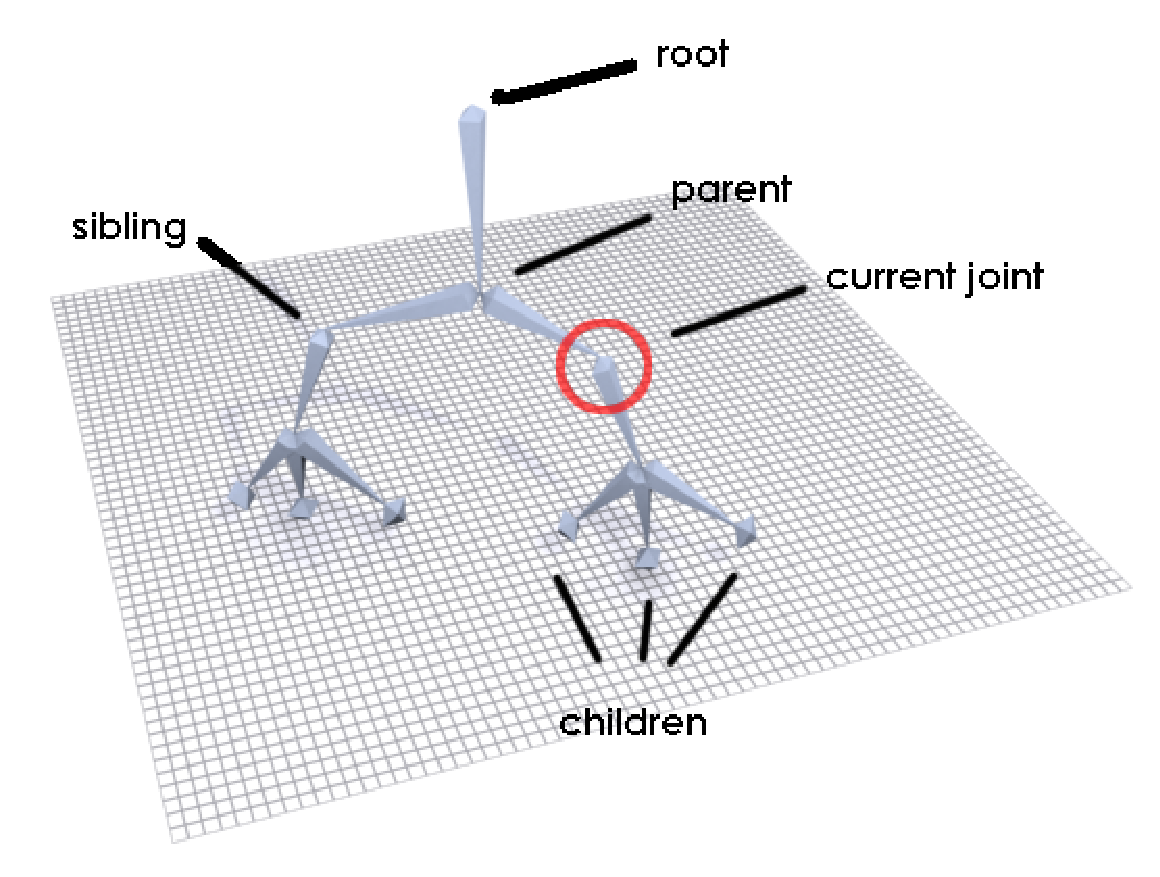
\includegraphics[scale=0.5]{pics/Skeleton.eps}
	\caption{Skeleton}
	\label{fig:Skeleton}
\end{figure}




\subsection{Animations}
Meshes can have morph target or skeletal\footnote{Also called, vertex/palette skinning} animations which can be mixed together. There's no limitation about the number of mixed animations, but try to avoid playing thousands of animations at the same time - the performance would be terrible. The animation playback itself is handled over a comfortable uniform animation interface.

You can use the \emph{GetAnimationsList()} function of the mesh handler to request a list of all available animations - note that there's no difference between morph target and skeleton animations. Because you as programmer should not be forced to create animations by self, that's the task of the graphic designer - this will safe you a lot of time! But the creation of own animations during runtime by hand is still possible. The animation resources are accessed through their names set by the designer like \emph{stand}, \emph{walk} an so on, they can be accessed trough their ID, too, but that's not recommended! To be able to playback such animation resources your mesh handler needs an animation manager which is a kind of mixer, it mixes the currently played animations to get a final result. The software animation manager is the default setting - this manager has no real limited features but it is using the \ac{CPU}. A hardware animation manager\footnote{Not yet implemented} would be another known alternative, which may have a better performance, but such managers normally have different limitations like a weights per vertex limit, a joint limit, active morph targets limit etc. The following example creates an animation manager instance if there's no one and start's the playback of all available animations:

\begin{lstlisting}[caption=Animation playback]
// Get/create the animation manager of our mesh handler
PLMesh::MeshAnimationManager *pAniManager = pMeshHandler->GetMeshAnimationManager();
if (!pAniManager)
	pAniManager = pMeshHandler->CreateMeshAnimationManager();
if (pAniManager) {
	// Get a list of all available animations
	PLCore::Array<PLCore::String> lstAnimations;
	pMeshHandler->GetAnimationsList(lstAnimations);
	for (PLCore::uint32 i=0; i<lstAnimations.GetNumOfElements(); i++) {
		PLMesh::AnimationInfo *pAniInfo = pMeshHandler->GetAnimationInfo(*lstAnimations[i]);
		PLMesh::Animation *pAni = pAniManager->Create(*lstAnimations[i]);
		if (pAniInfo && pAni)
			pAni->Start(pAniInfo);
	}
}
\end{lstlisting}

\begin{figure}
  \centering
  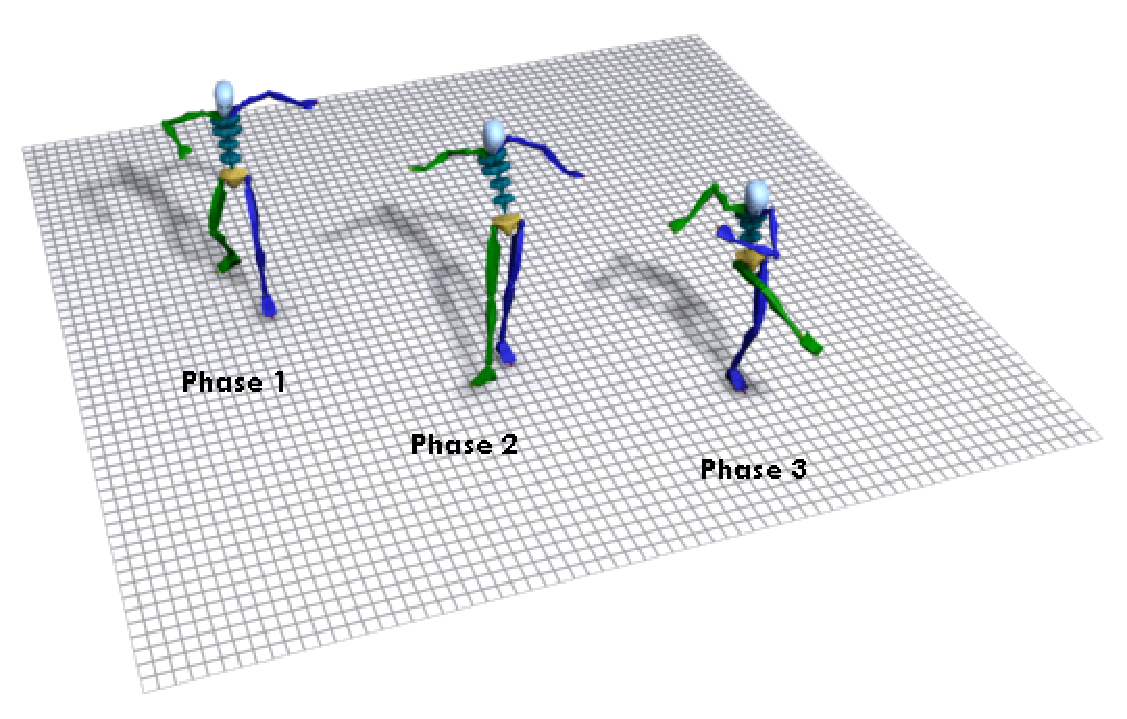
\includegraphics[scale=0.5]{pics/Joints.eps}
  \caption{Skeleton animation}
  \label{fig:Skeleton animation}
\end{figure}

\chapter{Contact}

\href{mailto:contact@pixellight.org}{contact@pixellight.org}\\
\url{http://www.pixellight.org}
	% "input" instead of "include" is used to avoid problems with write permissions during TeX processing


%----- End ---------------------------------------
\end{document}

\chapter{PLScene}


\paragraph{Motivation}
The \emph{PLScene} component is the place were the magic happens. While high level libraries like \emph{PLMesh} already made the daily life easier, a single mesh usually is not enough for most applications. Real world applications need to deal with complete scenes consisting of tons of meshes as well as rendering them. This is were \emph{PLScene} comes in. The main component within \emph{PLScene} is the scene graph - the scene graph is an representation of the scene


\paragraph{External Dependences}
PLScene depends on the \textbf{PLCore}, \textbf{PLMath}, \textbf{PLGraphics}, \textbf{PLRenderer} and \textbf{PLMesh} libraries.




% Include the other sections of the chapter
\chapter{Scene system}




\section{Overview}
The scene system is one of the main components of PixelLight because it brings together multiple components using a scene graph. Within this chapter you get an idea what the \emph{scene system} from PixelLight is and what components it consists of.

The PixelLight scene system is divided into 4 parts: nodes, hierarchies, queries and scene render queries were a renderer can be seen as an advanced scene query.

Each element in the scene is a node with position, scale and rotation. A container is derived from this base scene element and is able to manage sub nodes within it. (composite design pattern)

We decided against an explicit \emph{world space} design because this would restrict the possibilities especially for huge and dynamic worlds. Each node has an axis aligned bounding box in node object coordinate system - we refer to it as \emph{scene node space}. Also, the node will hold a version of this box in \emph{scene container space}. Each time, the position, scale, rotation or bounding box itself is manipulated, this container space bounding box must be recalculated internally - like the transform matrix. But this recalculation is only done \emph{on demand} - meaning, if you request the transform matrix or container space bounding box and this is \emph{out of data}, it's first updated before it's returned.

This is the base of the scene system - create a scene node container and add scene nodes into it - a node can also be a container with more nodes within it. Each node is relative to it's container node, move your container and all your nodes will \emph{automatically move} with it. If a scene node changes position, rotation and so on, events are generated other components can react on. A node can also have modifiers which adds new functionality - see it as a kind of multi inheritance. For instance you can add physical behaviour to a node by adding a physics body modifier - then this physics modifier will take over the control of position and rotation. Normally this modifier will also listening it's owner node by using events, if for instance the position of the node is changed using \emph{SetPosition()}, the physics modifier will update it's rigid body. In reverse, if the rigid body changes translation it informs the node - but this is another story.


\paragraph{Scene hierarchy}
Each container can have a hierarchy assigned to manage the sub-nodes in a more effective way. If such a hierarchy is created it will create sub-hierarchies basing on the volumes of the nodes within the container. If a certain spatial subdivision is reached such a sub hierarchy contains links to nodes within this sub-hierarchy volume. Therefore, if one or more nodes are manipulated in that way their position, scale, rotation or volume was changed the container hierarchy must be updated. If you have a lot of dynamic nodes you have to select a hierarchy type which can deal efficient with frequently changing nodes. This node/container/hierarchy combination can be seen as a database holding your scene description.


\paragraph{Scene query}
To access the \emph{scene database} you can use a query. For instance, if you want to know which nodes of the scene intersecting a line you can create a \emph{line intersection}-query, set the line start and end point and perform the query. Internally the query will now use the hierarchy of the root container and checks which which sub-hierarchies intersecting this line. If a sub-hierarchy with one or more nodes is found the query will inform it's event listeners about this nodes - were each node is only visited one time. We mentioned that because in fact, one node can be within different sub-hierarchies if the node volume is intersecting the volumes of different sub-hierarchies. If a container node is found this container will be traversed using it's own hierarchy, too. (recursive traverse)

The most queries are created and destroyed frequently - but some may exist over multiple frames or for the complete program life time. The general renderer query which offers different visibility determination techniques for instance is such a \emph{long life} query - because for some special visibility algorithms like \emph{coherent occlusion culling} information from the previous frame is used.

In general such a query informs you only about \emph{touched} nodes. For instance, if you want to know which node is the first intersecting this line you have to sort the resulting nodes by self.


\paragraph{Scene renderer}
As mentioned before, a scene renderer itself is also a kind of query. First, we define what we mean with the term \emph{scene renderer}. If something is drawn on the screen you will often read the word renderer - \emph{amazing per pixel lighting renderer}... but WHAT is a renderer, and can I eat it? You known that there are different graphics API's like OpenGL or Direct3D - we call them \emph{renderer API}. Their main task is to deal with render states, textures, shaders, primitives and so on - in short, the most basic rendering stuff. Ignore here that Direct3D is in fact a small framework itself with the possibility to also render whole complex meshes. The PixelLight renderer is a wrapper around this renderer APIs, so the user normally don't have to care about which renderer API is used internally and how for instance rendering into texture is managed internally. So, this renderer will only deal with the basics of rendering - it is NOT able to render large and complex scenes by self, it even does not know that where is something like a \emph{mesh} or a \emph{large scene}. It's world only consists of render states, textures, shaders, primitives and so on. :)

A scene renderer is using the \emph{scene database} (THE scene graph) you provided and the PixelLight renderer tries to visualize your scene in a performant and suitable manner. A very basic scene renderer will traverse your scene and draws each found node using the draw functions of the node interface - maybe before the node is drawn, someone is checking whether or not this node is potential visible by checking whether or not this node is within the camera frustum. But even it such a frustum intersection test is performed, for a large scene with some thousand of nodes this will be quite inefficent to \emph{touch} each node visible or not. The task of a \emph{real} scene renderer can be divided into two parts: visibility determination (optimal: frustum, occlusion \& lod processing) and rendering. If the scene renderer is using complex per pixel lighting, the rendering of the scene is different to the rendering of the basic scene using old fashioned fix pass rendering. Instead only calling the draw functions of the node interface this renderer must set the different render states, textures, shaders etc. by self and therefore the user itself has less control over the rendering itself. But here, such user limitations are required to overcome more complex rendering. Such a complex renderer normally comes with it's internal \emph{shader library} which offers certain shaders for different purposes. For instance shaders for different light types like spot, projective or volumetric light and per light type variations for different surfaces and shading. If the scene renderer should render something, it will \emph{look into} it's shader library to find a shader which fits the requirements. Here, the PixelLight materials are only a kind of \emph{would nice to have} wishes from the artist. If a material doesn't provide a normal map, there's no need to perform normal mapping. Instead a more simple and more performant shader can be chosen. Or if the surface should use nice environment mapping a special shader combination must be chosen by the renderer. As you see, this is a more advanced and not that universal topic - but  you have to make compromises if something should be able to look good and be fast at the same time. Therefore, for PixelLight we decided to implement this scene renderer as \emph{loose} plugins - \footnote{As nearly everything in PixelLight - thank's to the clever RTTI system} and usually, a scene renderer consists of several scene renderer passes, a realtime compositing.

So, there are different scene renderer for different requirements, each with other limitations - it's possible that you have to write/modify a scene renderer for your own project if the provided stuff doesn't match your requirements. Also, it's recommended to write multiple versions of one and the same renderer - like different versions of an advanced per pixel lighting renderer. One for the latest GPU generation which can profit of the latest shader generation and features - and one for older GPU generations with less render details and features so that your product will also run on this hardware. As mentioned, because of the GPU limitations and the different system specifications, it's impossible to create ONE universal scene renderer which supports the whole palette of GPU generations and different systems and can also be used for each scene for any project.\footnote{In Germany we would say to such a thing \emph{Eierlegende Wollmilch Sau}}




\section{Class name conventions}
In order to be able to know what exactly a file/class is for by only looking at the name, there's a name convention for the scene system relevant things:

\begin{tabular}{|p{2cm}|p{5cm}|p{7cm}|}
\hline
\textbf{Prefix} & \textbf{Derived from} & \textbf{Description}\\
\hline
SN  & SceneNode         & Scene node\\
\hline
SC  & SceneContainer    & Scene container\\
\hline
SNM & SceneNodeModifier & Scene node modifier \\
\hline
SH  & SceneHierarchy    & Scene hierarchy\\
\hline
SQ  & SceneQuery        & Scene query\\
\hline
SR  & RenderQuery       & Scene render query\\
\hline
\end{tabular}




\section{Scene context}
Equally to a renderer context, a scene context is an instance that brings together everything that depends on each other. Within scene nodes there may be rendering data like vertex data, so a scene context is using a render context. Besides the renderer context there are other components that are shared amongst all elements within a scene context like meshes. Scene context instances can't share data. For this reasons you usually have only one scene context within your project - else meshes, textures and so on are loaded multiple times.




\section{What's a scene node?}
All objects within your 3D environment are scene nodes. The most obvious example is an actor that moves through the world. But not each scene node has a mesh, lights, triggers etc. are also scene nodes... even load screens can be scene nodes! (but it does not mean that's the best solution) The most time you will spend in programming those elements for different purposes. If you programmed a scene node once you are able to it use for many things... you can even create new scene nodes using another scene node as basis. Or you are able to add new features to a scene node by adding scene node modifier. All scene nodes are managed automatically by a scene node container, using such a container you can e.g. create new scene nodes.




\section{Scene node names}
Because there can be multiple scene nodes in different scene containers with the same names we need a name convention for scene nodes. If you have a pointer to a container and want to get a scene node from it, one can use for instance \emph{pMyContainer->GetByName("MyNode")} without any troubles. If a camera should always look at a target scene node and both, the camera and the target scene nodes are in the same container, you can use \emph{pMyCamera->SetAttribute("TargetNode", "MyTargetNode")}\footnote{Just an example, the camera scene node does not offer this} and you will get the assumed result - your camera will look at the scene node \emph{MyTargetNode}. But what if you have multiple containers and you only know that there's a scene container children node or parent node which has a node with the name \emph{MyTargetNode} inside it, but you don't know the container name at the moment? The scene system overloads the virtual \emph{Get()}-function of the element manager template to deal with such situations - the \emph{Get()}-function of a scene container is not restricted to \emph{it's own nodes} but also to ALL scene nodes available. Therefore you can use \emph{absolute names} like \emph{Root.DefaultSceneRoot.Scene.MyTargetNode} or \emph{relative names} like \emph{Scene.MyTargetNode} if you currently \emph{in} a container which has a scene container named \emph{Scene} which has a scene node called \emph{MyTargetNode}.

Because this, you are NOT allowed to use \emph{.} characters within \emph{concrete} scene node names you can set for instance by using \emph{pMyNode->SetName("MyNode")}. Further the name \emph{Root} is NOT allowed for scene nodes, this name is reserved for the \emph{scene root container} of PixelLight you can request using \emph{SceneContext::GetRoot()} or by \emph{pMyContainer->GetByName("Root")}. The name of the this \emph{root scene container} can NOT be changed. \emph{pMyContainer->GetByName("Parent")} will return the parent scene container. \emph{pMyContainer->GetByName("Parent.MyNode")} returns the scene node \emph{MyNode} of the parent scene container. \emph{pMyContainer->GetByName("This")} will return \emph{pMyContainer}. The sample application \emph{PLDemoSimpleScene} shipped with the SDK contains some more name examples using a concrete scene.




\section{Create, manage and remove scene node instances}
OK, enough scene system theory - now to praxis. First at all, we need to create a scene context using an existing renderer context.

\begin{lstlisting}[caption=Creating a scene context instance]
SceneContext *pSceneContext = new SceneContext(cRendererContext);
\end{lstlisting}

Within a scene context, there's a root scene container holding ALL scenes. Do NEVER use this root scene directly, instead, add for instance a container and use this as your application scene:

\begin{lstlisting}[caption=Creating a new scene container instance]
SceneContainer *pContainer = pSceneContext->GetRoot()->Create("PLScene::SceneContainer");
\end{lstlisting}

As nearly anywhere in PixelLight the scene system is heavily using the RTTI - and the plugin stuff comes for free. If you are not familiar with the PixelLight runtime type information system (RTTI) it's time to read the RTTI documentation\footnote{\emph{PLCore}-documentation} NOW to understand what it is and how to work with it. Your nodes can be implemented within your executable or within in another shared library, there's no different. Just use the node class name, an optional node name and optional node variable parameters when adding a new node into your scene container. Variables that are not set have a default setting.

\begin{lstlisting}[caption=Creating a new scene node instance]
pContainer->Create("PLScene::SNPointLight", "PointLight", "Color=\"1.0 1.0 1.0\"");
\end{lstlisting}

This adds a node of the type \emph{PLScene::SNPointLight} with the (optional) name \emph{PointLight} and sets the light color (Color) to white (1.0, 1.0, 1.0).

Note that each scene node MUST have it's one, unique name within a scene container - but there can be different nodes with the same name within different containers. If the name is already used then a number will be added behind the name automatically. If no name is provided, the node name is generated automatically using the class name and a number behind it. The third parameter is for optional node parameters. This allows to to set up different registered node variables on creation. The function will return a pointer to the new node, or a null pointer if an error occurred. Because the nodes are managed by the container they are in, the returned node pointer is only used in special situations. Note that you should NEVER store a direct pointer to an node by self because it's possible that the node is removed and then the pointer is invalid! (that's the case for all resources!) Instead store the node name and request a pointer to the node if you need one with:

\begin{lstlisting}[caption=Requesting a scene node by name]
SceneNode *pNode = pContainer->GetByName("PointLight");
\end{lstlisting}

If you need this node frequently or if you have multiple containers it's the best to use an scene node handler which keeps track of the node.

\begin{lstlisting}[caption=Scene node handler]
SceneNodeHandler cNodeHandler;
cNodeHandler.SetElement(pNode);     // Set handled node
pNode = cNodeHandler.GetElement();  // Get handled node
\end{lstlisting}

DO NEVER define/embed nodes (like all resources) direct into classes like

\begin{lstlisting}[caption=Invalid scene node instance usage]
class MyClass {
  private:
    int       m_nCounter;
    SceneNode m_cMyNode;
}
\end{lstlisting}

Because this can, and certainly will, cause fatal errors were many will result in a mysterious behaviour or even crash's! Now, we want to have a mesh in our scene:

\begin{lstlisting}[caption=Creating a new scene node mesh instance]
pContainer->Create("PLScene::SNMesh", "Statue", "Position=\"0.0 0.0 5.0\" Rotation=\"0.0 180.0 0.0\" Mesh=\"Statue.3ds\" Flags=\"CalculateNormals\"");
\end{lstlisting}

Nothing new here. Create an instance of \emph{PLScene::SNMesh} which can deal with meshes, setup the position and rotation of the node, define the filename of the used mesh and tell the node that it should (re-)calculate normals for this mesh. Now we need a camera node which can be seen as your window into the scene and backup a pointer to it, we will need it soon:

\begin{lstlisting}[caption=Creating a new camera scene node instance]
SNCamera *pCamera = (SNCamera*)pContainer->Create("PLScene::SNCamera");
\end{lstlisting}

Can you already see this scene within your head? Hopefully not because there's no light within this scene! OK, let's create a light illuminating the scene:

\begin{lstlisting}[caption=Creating a new light scene node instance]
pContainer->Create("PLScene::SNPointLight", "Light");
\end{lstlisting}

Your basic scene now has all it needs - but how to render it? If one of the renderer surfaces like a window is updated/drawn it will inform it's event listeners about this action. Normally you have an event which will draw some nice things into this renderer surface. The framework itself provides a standard renderer surface painter called \emph{SPScene} were things like a scene root node, camera etc. is assigned to.

\begin{lstlisting}[caption=SPScene setup]
pSurfacePainter->SetRootContainer(pContainer);
pSurfacePainter->SetCamera(pCamera);
\end{lstlisting}

Remove a node by use the \emph{SceneNode::Delete()} function. This function will only mark the node as killed, it will be destroyed later by self.

\begin{lstlisting}[caption=Delete a scene node]
pNode->Delete();
\end{lstlisting}




\section{Scene file format}
PixelLight saves it's scenes within the XML (eXtensible Markup Language) scene format with the extension \emph{scene}. Here's a short example scene:

\begin{lstlisting}[caption=Scene file example]
<?xml version="1.0"?>
<Scene Version="1" Name="Scene" Hierarchy="PLScene::SHList">
  <Container Class="PLPhysics::SCPhysicsWorld" Name="PhysicsWorld" PhysicsAPI="PLPhysicsNewton::World">
    <Modifier Class="DoAnything"/>
    <Node Class="SNMyEye" Name="Hero" Position="-3.0 12.0 5.0" Scale="0.5 1.0 0.5">
      <Modifier Class="PLPhysics::SNMPhysicsBodySphere" Mass="1.0" Radius="1.0"/>
      <Modifier Class="PLEngine::SNMPhysicsCharacterController"/>
    </Node>
    <Node Class="PLScene::SNMesh" Position="1.0 0.0 0.0">
      <Modifier Class="PLPhysics::SNMPhysicsBodyBox" Mass="1.0" />
    </Node>
  </Container>
</Scene>
\end{lstlisting}

Here's another example using a scene node defined within another project:

\begin{lstlisting}[caption=Another scene file example]
<?xml version="1.0"?>
<Scene Version="1">
  <Node Class="PLScene::SNCamera" Name="Camera" Position="10.0 2.0 0.0" Rotation="0.0 -90.0 0.0" />
  <Node Class="PLParticleGroups::PGSmoke" Position="-50 0 -50" />
</Scene>
\end{lstlisting}

Because each scene itself is in fact a scene container you can also add nodes directly into the scene. And here's the general DTD (Document Type Definition) of this format:

\begin{lstlisting}[caption=Scene file format DTD]
<?xml version="1.0"?>
<!DOCTYPE Scene [
  <!ELEMENT Modifier EMPTY>
  <!ATTLIST Modifier Class CDATA #REQUIRED>
  <!ELEMENT Node (Modifier*)>
  <!ATTLIST Node Class CDATA #REQUIRED>
  <!ELEMENT Container (Modifier*, Node*, Container*)>
  <!ATTLIST Container Class CDATA #REQUIRED>
]>
\end{lstlisting}

In words: A scene consists of nodes, containers, modifiers and a hierarchy. Scene itself is a container. A node can have some modifiers changing their behaviour. Because a container is derived from node, it can also have modifiers, further it can contain nodes or other containers. At last you can specify a hierarchy for the container. This hierarchy is used for the spatial management of it's nodes. Each of this elements has an attribute with at least a class name defining what type of element should be used. Further, there can be a lot of further attributes depending on the used class.




\section{Scene node classes}
Each scene node is basing on a node class you create instances from. All this classes are derived from the PixelLight base node class called \emph{PLScene::SceneNode} and therefore all other classes have the full functionality of this base class! There are some framework node base classes like \emph{PLScene::SNLight} defined within the framework itself... but only the core stuff is fixed. There are also many tool-nodes within the different plugins shipped together with PixelLight. With this given tools you are able to create your first scene without any effort in just a few minutes. It's not recommended to manipulate this standard nodes because they will be updated together with the framework. The better way would be to derive this standard tool nodes like all other nodes to expand their functionality... or you take the node class as base of your own complete new node by coping it.




\section{Creating own scene node classes}
In the most cases you will create your own node classes for an unique behaviour by deriving them from other nodes... at least from \emph{PLScene::SceneNode}. Creating an own scene node class is quite simple:

\begin{lstlisting}[caption=Creating a new own scene node class]
#include <PLScene/Scene/SceneNode.h>

class FlickerLight : public PLScene::SceneNode {
};
\end{lstlisting}

It's not recommended to use your own constructors and destructor's in node classes, but this is possible, too. Use instead the offered virtual functions for initialization and de-initialization you will find in \emph{PLScene::SceneNode} for sure. Note that it's not allowed to derive a new node class from more that one base node class!

\begin{lstlisting}[caption=Invalid scene node class creating]
// Not allowed!!
class FlickerLight : public PLScene::SceneNode, public PLScene::SNLight {
};
\end{lstlisting}

This node class definition isn't complete yet. You still have to register your new class in the PixelLight plugin system to be able to create nodes using this class... (see next sections)




\section{Scene system and RTTI}


\subsection{Overview}
The next section will teach you how to use the PixelLight RTTI together with the scene system. In fact, there's no special RTTI stuff within the scene system and if you already read the RTTI documentation here's nothing new for you.


\subsection{Register scene node classes}
All nodes classes must be registered in the RTTI plugin system in order to be able to use them within the framework. If this nodes are defined within shared libraries all other programs using the framework are able to use this node class, too. For instance you can create instances of this scene nodes within the scene editor. The class registration is done through:

\begin{lstlisting}[caption=RTTI and own new scene node class]
class MyFlickerLight : public PLScene::SceneNode { 
  public:
    // Register new scene node class using RTTI macros

    // Define new RTTI class called 'MyFlickerLight' which is derived from 'PLScene::SceneNode'
	pl_class(PLS_RTTI_EXPORT, MyFlickerLight, "", PLScene::SceneNode, "My flicker light")
      // Your new node can be created public using the Create() function of a scene node container
		pl_constructor_0(DefaultConstructor, "Default constructor", "")
	pl_class_end

};
\end{lstlisting}

At last you have to add this into your node source file which completes the registration process:

\begin{lstlisting}[caption=Finishing RTTI class registration process]
pl_implement_class(MyFlickerLight)
\end{lstlisting}

Now you are able to call this new own class by name! To create a node using this class you have to do this:

\begin{lstlisting}[caption=Creating an instance of an own scene node class]
// pContainer is a scene node container
// created somewhere before
pContainer->Create("MyFlickerLight");
\end{lstlisting}

... easy, uh?

This node plugins are automatically managed by the framework and the classes can be used without any extra work. If the application path is set (done at program start automatically) the framework detects all plugins which are in this directory by self and because its possible to change the application path during runtime the plugings registered in the framework can change during runtime!




\section{Scene node meshes}
Normally it's recommended use scene nodes when dealing with meshes. There's a standard class named \emph{PLScene::SNMesh} with comes with a mesh interface by default. If a mesh is loaded the node function \emph{MeshInitFunction()} is called were you can initialize different mesh related stuff like animations. \emph{MeshDeInitFunction()} is called if the mesh get's unloaded.

Because normally you only work with the animations provided by the mesh handlers animation list it's a good idea to store direct pointers to the different animation information in order to increase code readability and performance! This should be done after to mesh was loaded, \emph{MeshInitFunction()} is predicted for such an usage. Example:

\begin{lstlisting}[caption=Derived mesh scene node]
class MyGoblin : public PLScene::SNMesh {

	pl_class(PLS_RTTI_EXPORT, MyGoblin, "", PLScene::SNMesh, "My goblin")
		pl_constructor_0(DefaultConstructor, "Default constructor", "")
	pl_class_end

  private:
    // Animations
    AnimationInfo *m_pStandAnimation,
                  *m_pRunAnimation;

  protected:
    virtual void MeshInitFunction();
    virtual void InitFunction();

}

void MyGoblin::MeshInitFunction()
{
  // Get the desired animations
  m_pStandAnimation = GetMeshHandler()->GetAnimationInfo("Stand");
  m_pRunAnimation = GetMeshHandler()->GetAnimationInfo("Run");
}

void MyGoblin::InitFunction()
{
  // Get/create the animation manager of your mesh handler
  MeshAnimationManager *pAniManager = GetMeshHandler()->GetMeshAnimationManager();
  if (!pAniManager)
    pAniManager = GetMeshHandler()->CreateMeshAnimationManager();

  // Start animation playback - we check whether the animation
  // is available  first... maybe the artist forgot it :)
  if (m_pStandAnimation) {
    // Add a concrete animation to the animation manager...
    Animation *pAni = pAniManager->Create(m_pStandAnimation->GetSourceName());

    // ... and start the playback of your stand animation now
    // if all went fine
    if (pAni)
      pAni->Start(m_pStandAnimation, true);
  }
}
\end{lstlisting}

In this example \emph{MyGoblin} is derived from \emph{PLScene::SNMesh} which loads a mesh if it's initialized and therefore \emph{MeshInitFunction()} is usually called before \emph{InitFunction()}. The animation start function will check automatically whether the given pointer is valid or not, meaning not a null pointer and therefore you don't have to test the pointer by self to ensure that no crash will occur if there wasn't an animation with the requested name! It's a good idea to write a warning message into the log if the desired animation wasn't found. There's a tool function called \emph{GetAnimationInfo()} in the interface of the mesh handler which will do this automatically. This function will return a pointer to the animation information with the given name. If no animation information with the given name was found a warning message can  be written into the log automatically. Note that the second function parameter is the debug mode were the log message will be written, this is set to 1 by default.


\subsection{Debug flags}
It's possible to visualize anchor points, joints, vertices etc. during runtime using the debug flags. This can be quite useful while debugging.

\cleardoublepage

\chapter{PLPhysics}


\paragraph{Motivation}
PixelLight itself has no own physics implementation nor even fixed build in physics support within the scene graph itself. Such a physics engine is an own complex task - and at the moment the PixelLight team has no possibility (lack of time and man-power) to write a complete own physics solution.

But there are ton's of physics libraries out there - many of them free or even open source and the most modern even with hardware support.

As mentioned above, PixelLight does not come with native physics support within the scene graph component itself - but through the carefully considered design of the PixelLight framework such an 'hacked in'-support is unnecessary, it would even waste the sweet universal design. Because of the extreme plugin nature of PixelLight, it's no problem to add something like physics to your projects.

The PixelLight \ac{SDK} itself comes with a few such physics plugins. By using this plugins it's extremely simple to add physics to your scene. In fact, this plugins only have one scene node container for the physics world/simulation and a few scene node modifier. Create a scene container using such a physics world scene node container class and add some scene nodes into it. For nodes which should have physical behaviour just add a physics body modifier to the node. If a body has no mass it's considered to be static... et voil�.

To connect two physics bodies you can add a joint modifier to one of the bodies and 'hang in' the second one into the joint. For more advanced physics control you have to use the functions of the physics \ac{API} of your choice directly - we decided against wrapping all these functions. This would be to much work and to less advanced because the physics \ac{API} differ at many points a lot of. It's impossible to create one universal interface for all physics \ac{API}s wrapping all available features.

You can use multiple physics \ac{API}s within your project at the same time, but this isn't recommended and doesn't make much sense - this different simulations also can't interact with each other. So, for your project, you normally have to choose one physics \ac{API} and use it for the hole project. Changing during development to another physics \ac{API} wouldn't be that easy. You can extent this PixelLight physics plugins by self (not recommended) or add a plugin for another physics \ac{API} if required.


\paragraph{External Dependences}
\emph{PLPhysics} depends on the \textbf{PLScene} library, and therefore an all other libraries \textbf{PLScene} depends on.




% Include the other sections of the chapter
\section{Physics Backends}
This section deals with the different physics backends shipping with the PixelLight SDK.


\paragraph{Null}
\begin{itemize}
\item The null physics backend does nothing - can be useful if you e.g. are in debug mode and don't want have any physics.
\item PixelLight component name: PLPhysicsNull
\item Used dll's: \emph{PLPhysicsNull.dll}
\end{itemize}


\paragraph{Newton Game Dynamics}
\begin{itemize}
\item This is the preferred physics plugin of the PixelLight team because Newton Game Dynamics\footnote{Newton Game Dynamics can be downloaded from \url{http://newtondynamics.com/}} is really easy to use, offers a lot of geometry and joint types by default, has a nice interface (in fact JUST one header) and some usefull tool functions. Also the community is very active.
\item PixelLight component name: PLPhysicsNewton
\item Used dll's: \emph{PLPhysicsNewton.dll} and \emph{newton.dll}
\end{itemize}


\paragraph{Open Dynamics Engine (ODE)}
\begin{itemize}
\item Currently not within the official PixelLight SDK
\item The Open Dynamics Engine\footnote{Open Dynamics Engine can be downloaded from \url{http://www.ode.org/}} or short ODE is a well-known open source physics engine.
\item PixelLight component name: PLPhysicsODE
\item Used dll's: \emph{PLPhysicsODE.dll} and \emph{ode.dll}
\end{itemize}


\paragraph{PhysX}
\begin{itemize}
\item Currently not within the official PixelLight SDK
\item PhysX\footnote{PhysX can be downloaded from \url{http://developer.nvidia.com/object/physx.html}} is a commercial multithreaded physics API with support for the physics GPU. Please keep in mind that the \emph{PhysX SDK System Software} must be installed to be able to use PhysX - this may not be acceptable for each project.
\item PixelLight component name: PLPhysicsPhysX
\item Used dll's: \emph{PLPhysicsPhysX.dll} and \emph{PhysXLoader.dll}
\end{itemize}

\cleardoublepage

\chapter{PLSound}


\paragraph{Motivation}
PixelLight itself has NO own sound implementation nor even fixed build in sound support within the scene graph itself. But there are ton's of sound libraries out there - many of them free or even open source. As mentioned before, PixelLight does not come with native sound support - but through the carefully considered design of the PixelLight framework such an 'hacked in'-support is unnecessary, it would even waste the sweet universal design. Because of the extreme plugin nature of PixelLight, it's no problem to add something like sounds to your projects.

The PixelLight SDK itself comes with a few such sound plugins. By using this plugins it's extremely simple to add sound to your scene. In fact, this plugins only have one scene node container for the sound world and a few scene node modifier. Create a scene container using such a sound world scene node container class and add some scene nodes into it. For nodes which should have sound behaviour just add a sound modifier to the node.

You can use multiple sound API's within your project at the same time, but this isn't recommended and doesn't make much sense. So, for your project, you normally have to choose ONE sound API and use it for the hole project. You can extent this PixelLight sound plugins by self (not recommended) or add a plugin for another sound API if required.


\paragraph{External Dependences}
\emph{PLSound} depends on the \textbf{PLScene} library, and therefore an all other libraries \textbf{PLScene} depends on.




% Include the other sections of the chapter
\chapter{Sound}




\section{Overview}
In PixelLight there's no difference between sound and music. Therefore we use only the term sound. The sound component is using backends like the renderer component to enable you to use whatever sound API you want to use. But unlike the renderer component no other PixelLight component depends on the sound component. It's possible to playback 2D and 3D sounds and different sounds and music can be mixed/blended together. Here's a digram the sound component look's like:\\
\begin{figure}
  \begin{center}
    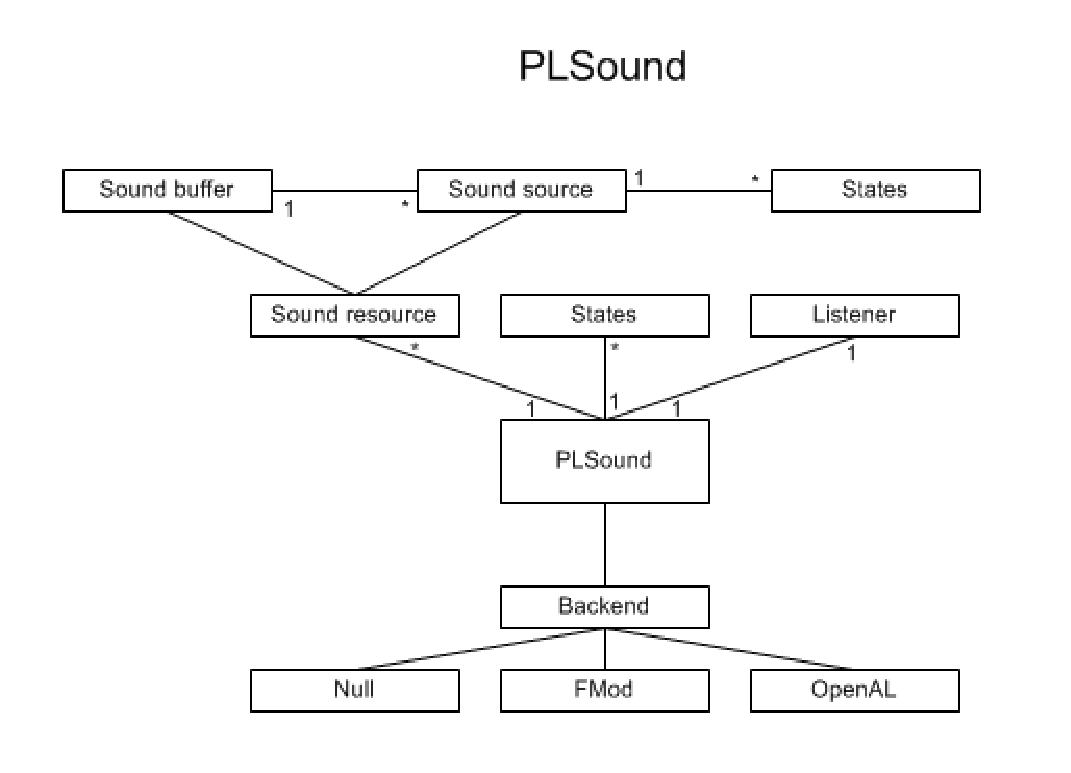
\includegraphics{pics/PLSoundClassDiagram.eps}
  \end{center}
  \caption{Sound component}
  \label{fig:Sound component high-level UML class diagram}
\end{figure}




\section{Sound scene node}
The sound component comes with a scene node called \emph{PLSound::SNSound} you can place into your scene for sound playback. There's also a scene node modifier called \emph{PLSound::SNMSound} if you just want to add sound to a scene node without adding a new one. The sound position is set by this scene node and will do all the dirty work for you, quite easy to deal with dynamic 3D sounds, eh?

This scene plugins can only be used correctly if they are placed inside a \emph{PLSound::SCSound} scene container - but it's not required that they are direct children and can be placed within any sub-container that's inside a sound scene container.

Have a look at the \emph{PLDemoSoundBasic} demo that comes with the PixelLight SDK.

\section{Sound Backends}
This section deals with the different sound backends shipping with the PixelLight SDK.


\paragraph{Null}
\begin{itemize}
\item The null sound backend does nothing - can be useful if you e.g. are in debug mode and don't want to hear any sounds.
\item PixelLight component name: PLSoundNull
\item Used dll's: \emph{PLSoundNull.dll}
\end{itemize}


\paragraph{OpenAL}
\begin{itemize}
\item OpenAL\footnote{OpenAL can be downloaded from \url{http://www.openal.org/}} backend with support of wav and ogg vorbis (streaming/no streaming) is provided.
\item PixelLight component name: PLSoundOpenAL
\item Used dll's: \emph{PLSoundOpenAL.dll}, \emph{OpenAL32.dll} and \emph{wrap\_oal.dll}
\end{itemize}


\paragraph{FMODEx}
\begin{itemize}
\item Currently not within the official PixelLight SDK
\item FMODEx\footnote{FMODEx can be downloaded from \url{http://www.fmod.org/}, only free for none commercial projects, \emph{FMOD Sound System, copyright � Firelight Technologies Pty, Ltd., 1994-2011.}} backend which can produce a lot of state of the art sound effects! Some of many supported formats are mp3, wav, mid, midi, it, mod, s3m, xm etc. 
\item PixelLight component name: PLSoundFMODEx
\item Used dll's: \emph{PLSoundFMODEx.dll} and \emph{fmodex.dll}
\end{itemize}


\paragraph{FMOD}
\begin{itemize}
\item Currently not within the official PixelLight SDK
\item FMOD\footnote{FMOD can be downloaded from \url{http://www.fmod.org/}, only free for none commercial projects, \emph{FMOD Sound System, copyright � Firelight Technologies Pty, Ltd., 1994-2011.}} backend which can produce a lot of state of the art sound effects! Some of many supported formats are mp3, wav, mid, midi, it, mod, s3m, xm etc. 
FMOD is the predecessor of FMODEx. Use the newer FMODEx if possible.
\item PixelLight component name: PLSoundFMOD
\item Used dll's: \emph{PLSoundFMOD.dll} and \emph{fmod.dll}
\end{itemize}

\cleardoublepage

\chapter{PLInput}


\paragraph{Motivation}
The PixelLight input component, or short \emph{PLInput}, provides access and control over several input devices. Although the purpose of this project is to have an input library that perfectly integrates into the PixelLight framework, \emph{PLInput} can be used without other PixelLight components like the rendering system as well.




\section{External Dependences}
The core of PLInput depends on the \textbf{PLCore} and \textbf{PLMath} libraries. PLInput is using some platform dependent third party libraries, but usually, the resulting binary of PLInput library is stand alone and does not force you to deliver additional shared libraries, too.


\paragraph{Microsoft Windows}
When compiling for \emph{Microsoft Windows}, there are no additional external dependencies - the few required \emph{hid.dll} system shared library functions are loaded dynamically.




\section{Important Terminology}
Within the PixelLight input system, there's some some important terminology we first need to define before we can go into details.


\paragraph{Controller, Controls, Buttons, Axis}
A \emph{controller} represents an input device, which can either be a real device like e.g. a mouse or joystick, or a virtual device that is used to map real input devices to virtual axes and keys. A controller consists of a list of \emph{controls}, e.g. \emph{buttons} or \emph{axes} and provides methods to obtain the status. While a button can be pressed, not not pressed, an axis has quantized values within a given interval.


\paragraph{Absolute And Relative Axis}
Depending on the input device and axis type, the value of an axis can be \emph{absolute} or \emph{relative}. A good example for an absolute axis is the x axis of a joystick. As long as you keep the joystick pulled to the left, you get a certain value. On the other hand, a mouse is a good example for a relative axis. If you move our mouse to the left, the position difference is recognized once, and send to the system. This means that the relative axis contains time information\footnote{The position difference of the mouse since the last position test some time ago} while a absolute axis contains no time information\footnote{Ignoring the fact that the axis value can change over time, but that's not interesting in here}. It's important to keep the time information in mind when using the device controls in order to, for instance, moving around a character.




% Include the other sections of the chapter
\section{Physical Input Devices}
\label{Chapter:PhysicalInputDevices}
This section deals with the actual, physical devices an, for instance human being, is using in the physical world in order to communicate with the computer. While starting with traditional input devices like the keyboard or the mouse, we also cover classic gaming devices like the joystick/gamepad and modern gaming devices like Wii Remote\footnote{Sometimes unofficially nicknamed \emph{Wiimote}}. Especially for developers, there are input devices like a space mouse making navigation within virtual worlds quite comfortable - therefore, they are covered as well.




\subsection{Keyboard}
As seen within source~code~\ref{Code:KeyboardUsageExample}, accessing a keyboard is quite simple.
\begin{lstlisting}[float=htb,label=Code:KeyboardUsageExample,caption={Keyboard usage example}]
// Get keyboard input device
Keyboard *pKeyboard = InputManager::GetInstance()->GetKeyboard();
if (pKeyboard) {
  // Update movement vector
  if (pKeyboard->KeyUp.IsPressed())
    vMovement += vDirVector;
  if (pKeyboard->KeyDown.IsPressed())
    vMovement -= vDirVector;
}
\end{lstlisting}




\subsection{Mouse}
As seen within source~code~\ref{Code:MouseUsageExample}, accessing a mouse is quite simple.
\begin{lstlisting}[float=htb,label=Code:MouseUsageExample,caption={Mouse usage example}]
// Get mouse input device
Mouse *pMouse = InputManager::GetInstance()->GetMouse();
if (pMouse && pMouse->Left.IsPressed()) {
  // Get the current time difference
  const float fTimeDiff = Timing::GetInstance()->GetTimeDifference();

  // Get mouse movement
  const float fX = pMouse->X.GetValue() * fTimeDiff;
  const float fY = pMouse->Y.GetValue() * fTimeDiff;

  // Get a quaternion representation of the rotation delta
  Quaternion qRotInc;
  EulerAngles::ToQuaternion(float(fX * Math::DegToRad),
                            float(fY * Math::DegToRad),
                            0.0f,
                            qRotInc);

  // Set new rotation
  qNewRotation = qOldRotation * qRotInc;
}
\end{lstlisting}




\subsection{Joystick}
When talking about \emph{joysticks}, we also cover \emph{gamepads} by this term because technically, their're practically the same. Therefore, when looking over the PixelLight input device classes, one may suspect that there's no support for gamepads, but that's not true because joysticks and gamepads are both handled by the joystick class.

As seen within source~code~\ref{Code:JoystickUsageExample}, accessing a joystick is quite simple.
\begin{lstlisting}[float=htb,label=Code:JoystickUsageExample,caption={Joystick usage example}]
Joystick *pJoystick = (Joystick*)InputManager::GetInstance()->GetDevice("Joystick0");
if (pJoystick && pJoystick->GetButtons()[0]->IsPressed()) {
  // Get the current time difference
  const float fTimeDiff = Timing::GetInstance()->GetTimeDifference();

  // Get joystick axis
  const float fX = pJoystick->X.GetValue() * fTimeDiff;
  const float fY = pJoystick->Y.GetValue() * fTimeDiff;

  // Get a quaternion representation of the rotation delta
  Quaternion qRotInc;
  EulerAngles::ToQuaternion(float(fX * Math::DegToRad),
                            float(fY * Math::DegToRad),
                            0.0f,
                            qRotInc);

  // Set new rotation
  qNewRotation = qOldRotation * qRotInc;
}
\end{lstlisting}




\subsection{Wii Remote}
As seen within source~code~\ref{Code:WiiRemoteUsageExample}, accessing a Wii Remote is quite simple.
\begin{lstlisting}[float=htb,label=Code:WiiRemoteUsageExample,caption={Wii Remote usage example}]
// Get Wii Remote input device
WiiMote *pWiiMote = (WiiMote*)InputManager::GetInstance()->GetDevice("WiiMote0");
if (pWiiMote && (pWiiMote->ButtonA.IsPressed())) {
  // Get the current time difference
  const float fTimeDiff = Timing::GetInstance()->GetTimeDifference();

  // Get orientation
  const float fX = float(pWiiMote->OrientX.GetValue() * fTimeDiff * Math::DegToRad);
  const float fY = float(pWiiMote->OrientY.GetValue() * fTimeDiff * Math::DegToRad);
  const float fZ = float(pWiiMote->OrientZ.GetValue() * fTimeDiff * Math::DegToRad);

  // Get a quaternion representation of the rotation delta
  Quaternion qRotInc;
  EulerAngles::ToQuaternion(fX, fY, fZ, qRotInc);

  // Set new rotation
  qNewRotation = qOldRotation * qRotInc;
}
\end{lstlisting}




\subsection{Space mouse}
Several space mouses from \emph{3DConnexion} are supported: \emph{SpaceMousePlus}, \emph{SpaceTraveler}, \emph{SpaceBall}, \emph{SpacePilot} and \emph{SpaceExplorer}.

Controlling an orbiting or free camera by using a space mouse is quite comfortable and is replacing mouse AND keyboard for this purpose.

As seen within source~code~\ref{Code:SpaceMouseUsageExample}, accessing a space mouse is quite simple.
\begin{lstlisting}[float=htb,label=Code:SpaceMouseUsageExample,caption={Space mouse usage example}]
// Get SpaceMouse device
InputManager *pInputManager = InputManager::GetInstance();
SpaceMouse *pSpaceMouse = (SpaceMouse*)pInputManager->GetDevice("SpaceMouse0");
if (pSpaceMouse) {
  // Get the current time difference
  const float fTimeDiff = Timing::GetInstance()->GetTimeDifference();

  // Get orientation
  const float fX = float(pSpaceMouse->RotX.GetValue() * fTimeDiff * Math::DegToRad);
  const float fY = float(pSpaceMouse->RotY.GetValue() * fTimeDiff * Math::DegToRad);
  const float fZ = float(pSpaceMouse->RotZ.GetValue() * fTimeDiff * Math::DegToRad);

  // Get a quaternion representation of the rotation delta
  Quaternion qRotInc;
  EulerAngles::ToQuaternion(fX, fY, fZ, qRotInc);

  // Set new rotation
  qNewRotation = qOldRotation * qRotInc;

  // Get translation
  const Vector3 vTrans(pSpaceMouse->TransX.GetValue() * fTimeDiff, pSpaceMouse->TransY.GetValue() * fTimeDiff, pSpaceMouse->TransZ.GetValue() * fTimeDiff);

  // Set new position
  vNewPos = vOldPos + vTrans;
}
\end{lstlisting}

\cleardoublepage
\section{Virtual Input Controllers}
Using physical input devices directly, as seen within chapter~\ref{Chapter:PhysicalInputDevices}, is quite comfortable and also an obvious way to deal with input devices - maybe that's the reason why most input systems out there just support this approach. While someone may be happy with this \emph{direct} solution for some time, there will probably come the point were the need arises to support multiple input devices to, for example, moving around a camera by the keyboard, the mouse, the joystick, the space mouse or by using all devices at once in a combination. A trivial solution for multi-input-devices-support would be, to just build in the support right at the place were it's required like
\begin{quote}if (WiiRemote) move with Wii Remote, if (Mouse) move with mouse, if (Joystick) move with joystick, else () bad luck my friend\end{quote}
Every time, support for another input device is required, the code is extended to cover this new input device as well. On the second thought, it may come into ones mind that this is not the perfect solution for the multi-input-devices-support - especially when the demand arises that the user should be able to configure the input controls dynamically... and by this we don't mean to just assign another keyboard key to an action, but to be able to assign a control of a totally different input device to this action, as well!

By using \emph{virtual input controllers} instead of input devices directly, the multi-input-devices-support and dynamic-user-configuration demands can be fulfilled at one and the same time.

\cleardoublepage

\chapter{PLEngine}




\section{PLInput}
\begin{itemize}
\item{Aimed at modern input devices (6DOF tracking devices)}
\item{The input component gives you a feature rich access to standard devices like keyboard, mouse and joystick/joypad}
\item{Wii Remote support}
\item{SpaceMouse (SpaceNavigator, SpacePilot and so on) support}
\item{Device output controls such as rumble and force-feedback effects as well as control over device LEDs}
\item{Internally HID, Bluetooth and special OS functionality is used}
\end{itemize}




\section{PLRenderer}
\begin{itemize}
\item{Dynamic API design\footnote{The PixelLight SDK comes with Null and OpenGL (using FreeType (\url{http://www.freetype.org/}) for font support) backends, within the repository there's also a OpenGL ES 2.0 backend and an experimental Direct3D 9 backend}}
\item{Multiple output windows}
\item{Render to texture (RTT, also rendering to floating-point for HDR buffer is possible)}
\item{Multiple render targets for rendering into different textures at the same time (MRT)}
\item{Primitives are drawn through vertex and index buffers for maximum performance}
\item{Vertex streaming for combining the data of different vertex buffers}
\item{1D, 2D (and rectangle), 3D and cube textures}
\item{Mipmaps and texture compression support. These can be created automatically on the fly or used from given dds data, for instance, for maximum control and best loading times.}
\item{Abstract GPU program interface with support for vertex, geometry and fragment shaders\footnote{The OpenGL renderer backend supports GLSL and Cg (\url{http://developer.nvidia.com/object/cg_toolkit.html}) as shader languages}}
\item{Fonts and draw helpers so it's easy to draw lines, images and so on}
\item{Interface for fixed functions to support legacy graphics cards without, or just limited shader support}
\item{A lot of standard functions like stencil, blend, fog, point sprites, anisotropic texture filtering and much more not worth to be mentioned in here because it's just standard must have stuff}
\item{GPU program generator class for �ber-shaders}
\end{itemize}


\subsection{Texturing}
\begin{itemize}
\item{Different texture creator plugins (for instance blank texture, normalization cube map, angle cube map...)}
\item{The image class of PLGraphics is used to load and save textures which makes things quite comfortable}
\item{Alpha blended textures which can be loaded through formats like tga automatically. It is also possible to define a color key by providing a RGB and tolerance value to describe transparent areas}
\item{Maximum texture size is only limited by hardware, today nearly every card has at least textures with a size of 2048x2048, a GeForce4 for instance has maximum texture size of 4096x4096... and ATI Radeon HD 5870 up to 16384x16384... }
\item{Textures are automatically resized through the framework if their size is too large for the given hardware or if its dimensions are invalid (no power of 2). Moreover, there is a texture quality option in the configuration where the user can change the texture quality in order to gain more performance}
\item{Procedural texturing}
\item{Different texture animation techniques are provided, e.g. changing textures, texture matrix and color animations for a maximum freedom of creativity}
\end{itemize}


\subsection{Materials \& effects}
\begin{itemize}
\item{PixelLight comes with a powerful material \& effect system which enables you to create amazing effects like Normal-Mapping etc.}
\item{Each material consists of different flexible properties like color, shininess etc.}
\item{In addition to the main effect properties, it is possible to setup a lot of options like blending, culling, polygon offset etc. for each material}
\item{You can use as many texture layers as supported by hardware. Today there are at least 2 texture layers available, but a GeForce4 for instance has 4 and the latest hardware even has up to 16! Each texture layer can be animated which opens a huge animation freeness.}
\item{The effect system supports different techniques (fallbacks), passes were you can assigned shaders to each pass etc.}
\end{itemize}




\section{PLMesh}


\subsection{Meshes}
\begin{itemize}
\item{Own flexible binary chunk based mesh format. The mesh library comes with different mesh import plugins for 3ds, lwo, ase, obj, smd, x (any many more) - through the nature of PixelLight it's no problem to implement more importer and exporter by self.}
\item{Meshes can consist of different geometries and therefore it's possible to have a mesh with different materials per geometry.}
\item{Mesh animations can be mixed together, therefore different animation channels for vertex and skeleton animations are provided per mesh}
\item{Different mesh creator plugins (for instance sphere, cube, cylinder, disk, torus...)}
\end{itemize}


\subsection{Animation system}
\begin{itemize}
\item{All animation types are handled equally, meaning that the same animation interface is used to control vertex, skeleton, texture etc. animation. So every animation type can be accessed in the same way and with the same features!}
\item{Animations can cause events at certain frames. Those events will be sent to their owner entity which can react on it}
\item{Vertex (morph targets, can for example be used for facial animations) and skeleton animation system with multiple weights per vertex}
\item{Blending of different animations}
\end{itemize}




\section{PLScene}


\subsection{Scene system}
The dynamic and universal hierarchical scene system consists of scene nodes and scene containers. (composite design pattern) A scene node is the most basic scene element, and a scene container manages such scene nodes. A scene container can also manage child scene containers for a hierarchical scene. Within a scene container, a scene hierarchy like a KD-tree can be used to manage/access the scene nodes in a more effective way. Scene queries operate on this scene description. For instance, there is a query which returns all scene nodes intersecting a line or plane set. To make the system more efficient, scene nodes can have different modifiers. For instance, you can use a physics scene node modifier to give your scene node a physical behaviour. Physics are NOT fixed build in the scene graph itself - it comes through such plugins to make the framework more universal.
\begin{itemize}
\item{Powerfull 'scene node modifier' concept allowing to add as many modifiers to scene nodes you want taking for instance control over the position of the node, controlling morph targets of meshes and so on - the possibilities are nearly unlimited!}
\item{Because the RTTI is used nearly everywhere in PixelLight, the scene system can be extended without any effort and components can be reused in other projects}
\item{KD-tree and list scene hierarchy plugins provided}
\item{Line/plane set intersection and culling queries provided as well as multiple other queries}
\item{Scenes can be rendered using no culling at all, frustum culling or coherent hierarchical occlusion culling for more complex scenes}
\item{A comfortable post process manager class and a lot of prepared post processing effects are provided. Adding bloom, grey scale or even visualizing the scene using ASCII characters is no problem at all. You can combine existing effects to create a new one.}
\item{Various useful scene nodes like camera, light, sky, terrain, ingame gui, mirror and so on are built in}
\item{The sky scene node comes with multiple sky layers and creates impressive animated and atmospheric backgrounds like hills, where slowly moving clouds appear behind them}
\item{The terrain scene node is using GeoMipMapping to create easily usable, impressive and large landscapes}
\item{The scene format is a simple XML text format and therefore it's nearly version change save}
\item{Lights can have coronas, lens flares or can even blind the screen looking into them! Lights can also project images over the scene, like a projector, which produces impressive effects! Because nearly all content in the framework is managed in the same way, you can also project a video texture over the scene where you will see a movie!}
\end{itemize}


\subsection{Compositing system}
Scenes are rendered using a realtime compositing system. For example a first layer may clear the screen color to black, another may write down depth information and ambient color, a next may add lighting, another one fog and so on. The system is using the PixelLight RTTI, as such, it's expandable and can be heavily configured\footnote{Adding new layers, changing layer order, changing layer attributes, everything directly while a program is running}.
\begin{itemize}
\item{There are fixed functions and shaders based compositing layers to support a broad range of graphics cards}
\item{Fixed function: For legacy hardware without shader support and just fixed build in graphics features}
\item{Forward: A classic forward renderer using shaders. Each object is drawn per light again.}
\item{Deferred: A modern deferred renderer approach performing for example lighting in image space}
\item{Scene rendering is usually using �ber-shaders to enable many shader features, while using just the currently required features}
\item{Several types of light sources: directional, omnidirectional, spot, omnidirectional projective and projective spot}
\item{Shadow mapping}
\item{Post process system with 'build in' effects like 'Depth Of Field' (DOF) and many effects as plugins}
\item{HDR, Reinhard tone mapping, light adaptation, HDR bloom}
\item{Glow}
\item{Volumetric light scattering and depth fog}
\item{Screen-Space Ambient Occlusion (SSAO) with implementations for HBAO\footnote{Horizon Based Ambient Occlusion} and HDAO\footnote{High Definition Ambient Occlusion}}
\item{Gamma correction}
\item{Layers with debug information like wireframe, scene node icons, scene node names and so on}
\item{Many material features like diffuse and opacity mapping, normal mapping, detail normal mapping, parallax mapping, two sided lighting, specular and gloss mapping, ambient occlusion mapping, light mapping, emissive mapping, glow mapping, fresnel reflection, spherical environment mapping, cubic environment mapping, reflectivity mapping}
\end{itemize}


\subsection{Particle groups}
\begin{itemize}
\item{Particle groups are usual scene nodes}
\item{They emit and manage particles. Each particle can be customized in an easy way in order to create unique effects}
\item{Each particle group can only have one material for all its particles for performance reasons. But because you are able to set the texture coordinates for each particle individually, you are able to put many different particle images into one texture and then cut them out to create fast and amazing particle effects}
\item{The texture coordinate setting of the particles can be done automatically. You only have to define the rows and columns of the single sub-textures in the main material and then you are able to set the used sub texture by its index. With this technique it is also possible to create particles with animated textures!}
\item{Because the material of the particle group itself can also be animated there are even more particle animation possibilities!}
\item{Advanced particle effects like distorted particles (beams, lasers etc), rotation of the individual particles, particles with individual orientation etc. are possible}
\item{Point sprite support for maximum performance}
\item{Because the RTTI is used, no extra particle editor is required - just tweak the variables}
\end{itemize}




\section{PLSound}
\begin{itemize}
\item{Abstract and universal sound API\footnote{The PixelLight SDK comes with Null and OpenAL (\url{http://www.openal.org/}) backends, within the repository are also experimental FMOD (\url{http://www.fmod.org/}) and FMOD Ex (\url{http://www.fmod.org/}) backends.}}
\item{2D and 3D sound}
\item{Streaming}
\item{Global volume and pitch control (for instance to slow down the sound playback)}
\end{itemize}




\section{PLPhysics}
\begin{itemize}
\item{Abstract and universal physics API\footnote{The PixelLight SDK comes with Null and Newton Game Dynamics (\url{http://www.newtondynamics.com/}) backends, within the repository are also experimental Open Dynamics Engine (\url{http://www.ode.org/}) and PhysX (\url{http://developer.nvidia.com/object/physx.html}, backends.}}
\item{Ragdoll scene node (also called 'online animation', 'articulated character')}
\item{Physics tool scene nodes}
\item{Physics tool scene node modifiers: Normally you add physics to a scene node by just adding a physics scene node modifier to it}
\end{itemize}




\section{PLEngine}


\begin{itemize}
\item{High-level application classes}
\item{Comfortable picking features}
\item{Screenshot tool class}
\end{itemize}

%----- Preamble ----------------------------------
\documentclass[a4paper,12pt]{book}
\usepackage[T1]{fontenc}
\usepackage[latin1]{inputenc}
\usepackage{color}
\usepackage{verbatim}
\usepackage{fancybox}
\usepackage[alsoload=binary, mode=text,loctolang={DE:german},decimalsymbol=comma]{siunitx}	% Units (bit, byte and so on)
\usepackage{../Common/Tools}
\usepackage{../Common/Styles}
\usepackage[dvipdfm]{graphicx}
\usepackage{textcomp}
\flushbottom

\sloppy	% Avoid writing over linebreak
\hbadness=10000
\clubpenalty = 10000 % schliesst Schusterjungen aus
\widowpenalty = 10000 % schliesst Hurenkinder aus

% Links
\usepackage[dvipdfm, colorlinks=true, urlcolor=black, linkcolor=black]{hyperref}
\urlstyle{same} % Use normal font for Urls
\usepackage[all]{hypcap} % Link to the image, not the image caption

% Table
\usepackage{tabularx}
\usepackage{threeparttablex}
\usepackage{booktabs}
\usepackage{ltxtable}

% Code listening
\usepackage{color,listings}
\definecolor{darkgreen}{rgb}{0,0.5,0}
\definecolor{lightgray}{gray}{0.95}
\lstset{language=C++,
captionpos=b,
frame=single,
basicstyle=\ttfamily,
keywordstyle=\color{blue},
commentstyle=\color{darkgreen},
stringstyle=\color{red},
backgroundcolor=\color{lightgray},
numbers=left,
numberstyle=\tiny,
numbersep=5pt,
breaklines=true,
showstringspaces=false,
columns=fullflexible,	% Please, don't change e.g. "export ANDROID_SDK=~/android-sdk-linux_x86" into "export ANDROID_SDK =~/ android -sdk - linux_x86"
tabsize=2,
emph={double,bool,int,unsigned,char,true,false,void},
emphstyle=\color{blue},
emph={Assert,Test},
emphstyle=\color{red},
emph={[2]\using,\#define,\#ifdef,\#endif}, emphstyle={[2]\color{blue}}
}
	% "input" instead of "include" is used to avoid problems with write permissions during TeX processing
\begin{document}


%----- Title -------------------------------------
%----- Title -------------------------------------
\thispagestyle{empty}
\begin{center}

{\Huge \textbf{PixelLight PLGui Documentation}}\\
%----- Title -------------------------------------
\thispagestyle{empty}
\begin{center}

{\Huge \textbf{PixelLight PLScene documentation}}\\
\input{../Common/Title}

\end{center}


\end{center}

\tableofcontents


%----- Document ----------------------------------
\chapter{Introduction}




\section{Overview}
PLGui is a highly flexible and portable GUI (graphical user interface) library that comes with a strictly object oriented API for the C++ language. It allows the creation of graphical user interfaces in an platform independent way while providing advanced features (docking windows, look\&feel, etc.) that work similar on every platform.

Once it is designed with the PLGui API, the same GUI can be used on every supported platform just by changing the backend for PLGui. It is even possible to use more than one PLGui backend at one time, e.g. one native backend (Microsoft Windows/Linux) for the application framework and a backend for ingame menus.

The PLGui library provides the common GUI elements (windows, dialogs, menus, etc.) and has a great number of controls and common dialogs that can be used. In addition to this it is easy to create own windows or controls that have a custom design and behaviour and can even make use of advanced features.




\section{Features}
Supported platforms:
\begin{itemize}
\item Microsoft Windows
\item Linux
\item PixelLight 3D Engine
\end{itemize}

\chapter{Contact}

\href{mailto:contact@pixellight.org}{contact@pixellight.org}\\
\url{http://www.pixellight.org}
	% "input" instead of "include" is used to avoid problems with write permissions during TeX processing


%----- End ---------------------------------------
\end{document}

\chapter{Contact}

\href{mailto:contact@pixellight.org}{contact@pixellight.org}\\
\url{http://www.pixellight.org}
	% "input" instead of "include" is used to avoid problems with write permissions d\textsl{}uring TeX processing
\cleardoublepage


%----- Appendix ----------------------------------
\appendix
\chapter{PLCore - Common Pitfalls}
\label{Appendix:CommonPitfalls}
This appendix presents common pitfalls you may step into, or already have. If you read this before using PixelLight, you may remember some of the written later and then avoiding problematic situations. If you're already working with PixelLight and currently there's a problem and you've got no idea what's wrong - this appendix may provide you with information which may help.


\paragraph{Class Constructor And Virtual Methods}
In C++, classes may not yet be fully initialized within the class constructor, therefore the usage of virtual methods is quite dangerous and should be avoided in general. This is also true when using RTTI features within class constructors, this should be avoided, too. A good concept is the use of lightweight constructors that just set class attributes to known states, but not performing tons of work within the constructor. \emph{Init-On-Use} and \emph{Lazy-Evaluation} design patterns are usually a good and less problematic approach to avoid class constructor relevant problems.


\paragraph{ClassManager::EventClassLoaded}
If the RTTI class manager adds new classes, a \emph{ClassManager::EventClassLoaded} event is generated. Please note: At the time you receive this event, the class may not yet be fully initialized. For example, there may still class attributes missing. As a result, when catching the mentioned event, be carefully what you're doing with the new class. A good idea would be do set some \emph{dirty state} and then using a \emph{Init-On-Use} design pattern to initialize features depending on the new class as soon as they are used the first time.


\paragraph{RTTI Method And String Reference Parameter}
\label{Appendix:CommonPitfalls:RTTIMethodStringReferenceParameter}
Within PixelLight, when using strings as parameters we're usually using a reference to strings like \begin{quote}void MyFunction(const PLCore::String \&sString) \{ /* ... */ \}\end{quote}. The example function can then be called by writing for instance \begin{quote}MyFunction("My string");\end{quote} and all works as expected. When using a string reference as a parameter to a RTTI method, described within \ref{ClassMembers:Method}, one has to look out when dynamically calling the RTTI method. Have a look at the following example source~code~\ref{Code:ProblematicRTTIMethodStringReferenceDefinition}.
\begin{lstlisting}[label=Code:ProblematicRTTIMethodStringReferenceDefinition,caption={Problematic RTTI method and string reference parameter definition}]
// Class definition of MyClass
#include <PLCore/Base/Object.h>
class MyClass : public PLCore::Object {

	// RTTI interface
	pl_class(pl_rtti_export, MyClass, "", PLCore::Object, "Description of my RTTI class")
		pl_constructor_0(MyConstructor, "Default constructor", "")
		pl_method_1(MyMethod, bool, PLCore::String&, "My method", "")
	pl_class_end

	public:
		MyClass() : MethodMyMethod(this) {}
		bool MyMethod(PLCore::String &sMyString) {
			return true;
		}

};

// MyClass RTTI implementation
pl_implement_class(MyClass)
\end{lstlisting}
Looks intuitive, isn't it? The next source~code~\ref{Code:ProblematicRTTIMethodStringReferenceUsage} shows how one may intuitively call the RTTI method dynamically.
\begin{lstlisting}[label=Code:ProblematicRTTIMethodStringReferenceUsage,caption={Problematic RTTI method and string reference parameter usage}]
// Get RTTI class description
const PLCore::Class *pMyClass = PLCore::ClassManager::GetInstance()->GetClass("MyClass");
if (pMyClass != nullptr) {
	// Create an instance of the RTTI class
	MyClass *pMyObject = (MyClass*)pMyClass->Create();

	// Call a RTTI method
	pMyObject->CallMethod("MyMethod", "Param0=\"My string\"");

	// Cleanup
	delete pMyObject;
}
\end{lstlisting}
Still looks fine, isn't it? But probably, the programmer indented another behaviour in this case. As described within this document, the RTTI is type safe. Within the source~code~\ref{Code:ProblematicRTTIMethodStringReferenceDefinition} the RTTI method \emph{MyMethod} was defined with a \emph{PLCore::String\&} parameter, this means, a reference to a string object. But within source~code~\ref{Code:ProblematicRTTIMethodStringReferenceUsage} the RTTI method was called by writing \begin{quote}pMyObject->CallMethod("MyMethod", "Param0="My string"");\end{quote}. The method parameter \begin{quote}Param0="My string"\end{quote} implies that the first parameter of the method to call is of the type \emph{PLCore::String}, but this isn't the case, the type of the method parameter is in fact \emph{PLCore::String\&}. Because the RTTI method parameter is a reference, the RTTI is interpreting the given \emph{Param0} value as a reference, meaning a memory address. Unfortunately, for the most computer systems, \emph{"My string"} is no valid memory address. In short, the result won't be the same as one intuitively expected and the result is probably an ugly crash. Because in this example, the RTTI method takes a reference to a string, a reference to a string must be provided as shown within source~code~\ref{Code:CorrectRTTIMethodStringReferenceUsage}.
\begin{lstlisting}[label=Code:CorrectRTTIMethodStringReferenceUsage,caption={Correct RTTI method and string reference parameter usage}]
// Get RTTI class description
const PLCore::Class *pMyClass = PLCore::ClassManager::GetInstance()->GetClass("MyClass");
if (pMyClass != nullptr) {
	// Create an instance of the RTTI class
	MyClass *pMyObject = (MyClass*)pMyClass->Create();

	// Call a RTTI method
	PLCore::String sMyString = "My string";
	pMyObject->CallMethod("MyMethod", "Param0=\"" + PLCore::Type<PLCore::String&>::ConvertToString(sMyString) + "\"");

	// Cleanup
	delete pMyObject;
}
\end{lstlisting}
The RTTI method is now called correctly with the memory address of \emph{sMyString}, and the content of the string object, we're referencing to, is \emph{"My string"}. This described problematic situation is no bug or a result of a bad RTTI design, in fact, the shown code works absolutely correct and is consistent. A reference is a reference, whether it's a reference to a file object, or a reference to a string object doesn't matter to the RTTI. But usually, if a programmer reads \emph{string parameter}, something like \emph{"My string"} as value comes into the mind - which may result in a wrong usage of the system. Therefore, when using RTTI methods, we recommend to not use string reference parameters when it's not required. Just use string objects as parameters directly and the described situation, when dynamically calling the RTTI method in an intuitive way, does not occur. Internally, the \emph{PLCore::String} implementation is using the \emph{copy-on-write} design pattern, as a result, using string objects directly as parameters won't result in a complete copy of the string, internally, just a pointer to the internal string object is copied and then shared as long as possible. Nothing with an enormous impact on the runtime performance.

\cleardoublepage
\chapter{PLCore - User Defined RTTI Data Type}
\label{Appendix:UserDefinedRTTIDataType}
Although the RTTI comes with many standard RTTI data types, additional data types can be defined as well. In here, we create a user defined data type to show how this is done. Please note that this data type is not totally serious and we think it's possible to write applications without the use of this data type. We implement a \emph{troll} data type which is able to remember a complete number, as long as it's 0, 1 or 2 - in short: a completely useless example data type. The data type is defined within the source~codes~\ref{Code:UserDefinedRTTIDataTypeHeader}, \ref{Code:UserDefinedRTTIDataTypeInline} and \ref{Code:UserDefinedRTTIDataTypeSource}.

The new RTTI data type can then be used like all the other data types as shown within source~code~\ref{Code:UserDefinedRTTIDataTypeClassDefinition}.
\begin{lstlisting}[label=Code:UserDefinedRTTIDataTypeClassDefinition,caption={RTTI class using a user defined RTTI data type}]
// Class definition of MyClass
#include <PLCore/Base/Object.h>
class MyClass : public PLCore::Object {

	// RTTI interface
	pl_class(MY_RTTI_EXPORT, MyClass, "", "PLCore::Object", "Description")
		pl_constructor_0(MyConstructor, "Default constructor", "")
		pl_attribute(MyTroll, TrollType, TrollType(1), ReadWrite, DirectValue, "A troll, don't feed him!", "")
	pl_class_end

	// Default constructor
	public:
		MyClass() : MyTroll(this) {}

};

// MyClass RTTI implementation (not done within headers)
pl_implement_class(MyClass)
\end{lstlisting}
The RTTI class containing a user defined RTTI data type can than be used as seen within source~code~\ref{Code:UserDefinedRTTIDataTypeClassDefinition}.
\begin{lstlisting}[label=Code:UserDefinedRTTIDataTypeClassUsage,caption={Using a RTTI class containing a user defined RTTI data type}]
// Get RTTI class description
const PLCore::Class *pMyClass = PLCore::ClassManager::GetInstance()->GetClass("MyClass");
if (pMyClass != nullptr) {
	// Create an instance of the RTTI class
	MyClass *pMyObject = (MyClass*)pMyClass->Create();
	if (pMyObject != nullptr) {
		// Ask the troll about the number he should currently
		// remember -> sNumber is now "one"
		PLCore::String sNumber = pMyObject->MyTroll.GetString();

		// Give the smart troll a new number to remember
		pMyObject->MyTroll.SetInt(42);

		// Ask the troll about the number he should currently
		// remember -> sNumber is now "many"... because the troll
		// is only able to remember a number as long as it's 0, 1
		// or 2, he has better things do to than remembering huge
		// numbers...
		sNumber = pMyObject->MyTroll.GetString();

		// Cleanup
		delete pMyObject;
	}
}
\end{lstlisting}


\paragraph{Header Of The User Defined RTTI Data Type}
\begin{lstlisting}[label=Code:UserDefinedRTTIDataTypeHeader,caption={Header of the user defined RTTI data type}]
#pragma once

// Includes
#include <PLCore/Base/Type/Type.h>

// Classes
class TrollType {

	// Public functions
	public:
		TrollType();
		TrollType(int nValue);
		TrollType(const TrollType &cOther);
		~TrollType();
		TrollType &operator =(const TrollType &cOther);
		bool operator ==(const TrollType &cOther) const;
		int GetValue() const;
		void SetValue(int nValue);
		PLCore::String GetComment() const;

	// Private data
	private:
		int m_nValue;

};

// Include type implementation
#include "TrollType.inl"
\end{lstlisting}


\paragraph{Inline Of The User Defined RTTI Data Type}
\begin{lstlisting}[label=Code:UserDefinedRTTIDataTypeInline,caption={Inline of the user defined RTTI data type}]
#pragma once

// Namespace
namespace PLCore {

// Classes
template <>
class Type<TrollType> {

	// Public static type information
	public:
		typedef TrollType _Type;
		typedef TrollType _StorageType;
		static const int TypeID = 100101;
		static String GetTypeName() {
			return "troll";
		}
		static TrollType ConvertFromVar(const DynVar *pVar) {
			TrollType cTroll;
			cTroll.SetValue(pVar->GetInt());
			return cTroll;
		}
		static bool ConvertToBool(const TrollType &cTroll) {
			return (bool)(cTroll.GetValue() != 0);
		}
		static TrollType ConvertFromBool(bool bValue) {
			TrollType cTroll;
			cTroll.SetValue((int)bValue);
			return cTroll;
		}
		static int ConvertToInt(const TrollType &cTroll) {
			return cTroll.GetValue();
		}
		static TrollType ConvertFromInt(int nValue) {
			TrollType cTroll;
			cTroll.SetValue(nValue);
			return cTroll;
		}
		static int8 ConvertToInt8(const TrollType &cTroll) {
			return (int8)ConvertToInt(cTroll);
		}
		static TrollType ConvertFromInt8(int8 nValue) {
			return ConvertFromInt((int)nValue);
		}
		static int16 ConvertToInt16(const TrollType &cTroll) {
			return (int16)ConvertToInt(cTroll);
		}
		static TrollType ConvertFromInt16(int16 nValue) {
			return ConvertFromInt((int)nValue);
		}
		static int32 ConvertToInt32(const TrollType &cTroll) {
			return (int32)ConvertToInt(cTroll);
		}
		static TrollType ConvertFromInt32(int32 nValue) {
			return ConvertFromInt((int)nValue);
		}
		static int64 ConvertToInt64(const TrollType &cTroll)
		{
			return (int64)ConvertToInt(cTroll);
		}
		static TrollType ConvertFromInt64(int64 nValue)
		{
			return ConvertFromInt((int)nValue);
		}
		static uint8 ConvertToUInt8(const TrollType &cTroll) {
			return (uint8)ConvertToInt(cTroll);
		}
		static TrollType ConvertFromUInt8(uint8 nValue) {
			return ConvertFromInt((int)nValue);
		}
		static uint16 ConvertToUInt16(const TrollType &cTroll) {
			return (uint16)ConvertToInt(cTroll);
		}
		static TrollType ConvertFromUInt16(uint16 nValue) {
			return ConvertFromInt((int)nValue);
		}
		static uint32 ConvertToUInt32(const TrollType &cTroll) {
			return (uint32)ConvertToInt(cTroll);
		}
		static TrollType ConvertFromUInt32(uint32 nValue) {
			return ConvertFromInt((int)nValue);
		}
		static uint64 ConvertToUInt64(const TrollType &cTroll)
		{
			return (uint64)ConvertToInt(cTroll);
		}
		static TrollType ConvertFromUInt64(uint64 nValue)
		{
			return ConvertFromInt((int)nValue);
		}
		static uint_ptr ConvertToUIntPtr(const TrollType &cTroll)
		{
			return (uint_ptr)ConvertToInt(cTroll);
		}
		static TrollType ConvertFromUIntPtr(uint_ptr nValue)
		{
			return ConvertFromInt((int)nValue);
		}
		static float ConvertToFloat(const TrollType &cTroll) {
			return (float)cTroll.GetValue();
		}
		static TrollType ConvertFromFloat(float fValue) {
			TrollType cTroll;
			cTroll.SetValue((int)fValue);
			return cTroll;
		}
		static double ConvertToDouble(const TrollType &cTroll) {
			return (double)cTroll.GetValue();
		}
		static TrollType ConvertFromDouble(double dValue) {
			TrollType cTroll;
			cTroll.SetValue((int)dValue);
			return cTroll;
		}
		static String ConvertToString(const TrollType &cTroll) {
			return cTroll.GetComment();
		}
		static TrollType ConvertFromString(const String &sString) {
			TrollType cTroll;
				 if (sString.CompareNoCase("nuthin'"))	cTroll.SetValue(0);
			else if (sString.CompareNoCase("one"))		cTroll.SetValue(1);
			else if (sString.CompareNoCase("two"))		cTroll.SetValue(2);
			else if (sString.CompareNoCase("many"))		cTroll.SetValue(3);
			else										cTroll.SetValue(-1);
			return cTroll;
		}
		static TrollType &ConvertRealToStorage(TrollType &cValue) {
			return cValue;
		}
		static TrollType &ConvertStorageToReal(TrollType &cValue) {
			return cValue;
		}

};

// Namespace
} // PLCore
\end{lstlisting}
Please note that the declaration of new RTTI data types, in this case \emph{Type<TrollType>} must happen within the \emph{PLCore} namespace. If you don't do it this way, it may work on the \emph{Microsoft Visual Studio Compiler} but may fail on the \emph{gcc compiler for Linux}.


\paragraph{Source Of The User Defined RTTI Data Type}
\begin{lstlisting}[label=Code:UserDefinedRTTIDataTypeSource,caption={Source of the user defined RTTI data type}]
// Includes
#include "TrollType.h"

// Namespace
using namespace PLCore;

// Public functions
TrollType::TrollType() :
	m_nValue(0) {
}

TrollType::TrollType(int nValue) :
	m_nValue(0) {
	SetValue(nValue);
}

TrollType::TrollType(const TrollType &cOther) :
	m_nValue(cOther.m_nValue) {
}

TrollType::~TrollType() {
}

TrollType &TrollType::operator =(const TrollType &cOther) {
	m_nValue = cOther.m_nValue;
	return *this;
}

bool TrollType::operator ==(const TrollType &cOther) const {
	return (m_nValue == cOther.m_nValue);
}

int TrollType::GetValue() const {
	// Return value
	return m_nValue;
}

void TrollType::SetValue(int nValue) {
	// Try to remember value ...
	if (nValue >= 0 && nValue <=2)	m_nValue = nValue;
	else if (nValue > 2)			m_nValue =  3;
	else							m_nValue = -1;
}

String TrollType::GetComment() const {
	// Return comment about current value
		 if (m_nValue == 0)	return "nuthin'";
	else if (m_nValue == 1)	return "one";
	else if (m_nValue == 2)	return "two";
	else if (m_nValue  > 0)	return "many";
	else					return "wuz?";
}
\end{lstlisting}

\cleardoublepage
\chapter{PLCore - \ac{RTTI} Annotations}
\label{Appendix:RTTIAnnotations}
\ac{RTTI} objects like attributes have a string for optional annotations. In here, additional information or hints about the \ac{RTTI} objects can be provided. Within the \ac{RTTI}, the annotation has no build in meaning. Use annotations to denote for example control information for a \ac{GUI} system, like a minimum/maximum value or whether or not a string is used as a filename, so a \ac{GUI} can offer the user a file dialog.

Table~\ref{Table:PixelLightAnnotations} shows annotation semantics used across PixelLight itself:
\begin{table}[htb]
	\centering
	\begin{tabular}{|l|p{0.88\textwidth}|}
		\hline
		\textbf{Name} & \textbf{Semantic}\\
		\hline
		\hline
		Min  & Minimum allowed value. Example: \emph{Min=`0 1 2`} or \emph{Min=`-1`}\\
		\hline
		Max  & Maximum allowed value. Example: \emph{Max=`0 1 2`} or \emph{Max=`1`}\\
		\hline
		Inc  & For instance for spinner increase/decrease speed, default value is $0.1$. Example: \emph{Inc=5} or \emph{Inc=`0.2`}\\
		\hline
		Ext  & Valid filename extensions. Example: \emph{Ext=`mat jpg bmp`}\\
		\hline
		Type & Denotes the type of a resource that can be used. Example \emph{Type='Image'} to denote that it's a loadable resource of the type \emph{Image} or \emph{Type='Material Effect Image TextureAni'}.\\
		\hline
	\end{tabular} 
	\caption{PixelLight annotations for \emph{<name>=<value>}}
	\label{Table:PixelLightAnnotations}
\end{table}

\cleardoublepage



%----- Image index -------------------------------
% \addcontentsline{toc}{chapter}{\listfigurename}
% \listoffigures


%----- Table index -------------------------------
\addcontentsline{toc}{chapter}{\listtablename}
\listoftables


%----- Source code index -------------------------
\addcontentsline{toc}{chapter}{\lstlistlistingname}
\lstlistoflistings


%----- Abbreviations index -----------------------
\chapter*{Abbreviations}
\addcontentsline{toc}{chapter}{Abbreviations}
\begin{acronym}
	\setlength{\itemsep}{-\parsep}

	\acro{FAQ}{Frequently Asked Questions}
	\acro{DLL}{Dynamic-Link Library\acroextra{, under Linux it's called \ac{SO}}}
	\acro{SO}{Shared Object\acroextra{, under MS Windows it's called \ac{DLL}}}
	\acro{API}{Application Programming Interface}
	\acro{SDK}{Software Development Kit\acroextra{, also known as \emph{devkit}}}
	\acro{DOM}{Document Object Model}
	\acro{XML}{eXtensible Markup Language}
	\acro{OS}{Operating System}
	\acro{GPU}{Graphics Processing Unit}
	\acro{CPU}{Central Processing Unit}
	\acro{GUI}{Graphical User Interface}
	\acro{UI}{User Interface}
	\acro{RTTI}{Run-Time Type Information\acroextra{, or Run-Time Type Identification}}
	\acro{ODE}{Open Dynamics Engine}
	\acro{NSIS}{Nullsoft Scriptable Install System}
	\acro{MSVC}{Microsoft Visual C++\acroextra{, also known as \emph{Visual C++} or \emph{VC++}}}
	\acro{MFC}{Microsoft Foundation Class Library}
	\acro{GCC}{GNU Compiler Collection\acroextra{, formerly the "GNU C Compiler"}}
	\acro{HTML}{Hypertext Markup Language}
	\acro{URL}{Uniform Resource Locator}
	\acro{CSS}{Cascading Style Sheets}
	\acro{ASSIMP}{Open Asset Import Library}
	% Graphics
	\acro{HDR}{High Dynamic Range}
	\acro{HDRR}{High Dynamic Range Rendering}
	\acro{LDR}{Low Dynamic Range}
	\acro{DOF}{Depth Of Field}
	\acro{IBL}{Image Based Lighting}
	\acro{SSAO}{Screen-Space Ambient Occlusion}
	\acro{HBAO}{Horizon Based Ambient Occlusion}
	\acro{HDAO}{High Definition Ambient Occlusion}
	\acro{AO}{Ambient Occlusion}
	\acro{GLSL}{OpenGL Shading Language\acroextra{, also known as GLslang}}
	\acro{HLSL}{High Level Shader Language}
	\acro{VBO}{Vertex Buffer Object}
	\acro{IBO}{Index Buffer Object}
	\acro{UBO}{Uniform buffer\acroextra{, also known as constant buffer}}
	\acro{RTT}{Render To Texture}
	\acro{MRT}{Multiple Render Targets}
	\acro{POT}{Power-Of-Two}
	\acro{NPOT}{Non-Power-Of-Two}
	\acro{GBuffer}{Geometry Buffer}
	% Java
	\acro{JDK}{Java Development Kit}
	\acro{JRE}{Java Runtime Environment}
	% Android
	\acro{NDK}{Android Native Development Kit}
	\acro{APK}{Android Application Package file}
	% PixelLight
	\acro{PL}{PixelLight}

\end{acronym}
	% "input" instead of "include" is used to avoid problems with write permissions d\textsl{}uring TeX


%----- End ---------------------------------------
\end{document}
